\documentclass[12pt]{article}

\usepackage{amsmath}
\usepackage{graphicx}
\graphicspath{ {Figures/} }
\usepackage{amssymb}
\usepackage{textcomp}
\usepackage{gensymb}
\usepackage{bigints}
\usepackage{booktabs}
\usepackage{xcolor}
\usepackage{float}
\usepackage{caption}
\usepackage{natbib}
\usepackage[nottoc,numbib]{tocbibind} 
\setcitestyle{citesep={;}}
\renewcommand\bibname{References}
\usepackage[parfill]{parskip}
\usepackage{indentfirst}
\setlength{\parindent}{2em}
\usepackage{helvet}
\usepackage[section]{placeins}
\renewcommand{\familydefault}{\sfdefault}
\usepackage{fancyhdr}
\setlength{\headheight}{15pt} 
\pagestyle{fancy}
\rhead{Keegan Valerio}
\lhead{P-Sv Synthetic Seismograms}
\usepackage{hyperref}

\begin{document}
\title{Creating Synthetic Seismograms for Multicomponent P-Sv Reflection Seismic: Comparing Finite-Difference and Ray-Tracing Methods}
%\date{April 12, 2019}
\author{Keegan Valerio \\ \bigskip 10125114\\ GOPH 509\\University of Calgary}
\maketitle
\pagenumbering{gobble}
\clearpage

\pagenumbering{roman}
\tableofcontents
\pagebreak
\pagenumbering{arabic}

\listoffigures
\pagebreak

\section{Abstract}
	Synthetic seismograms are used to relate well data in the depth domain to seismic reflection data in the time domain. The simple convolutional model that is commonly used to generate synthetic seismograms is not effective for the P-Sv case since as the offset of a P-Sv reflection approaches zero, the amplitude also approaches zero. Multicomponent reflection seismic data is becoming increasingly common and as such, it is becoming increasingly important to have a reliable and accurate method of generating synthetics for this data.
	Finite-difference and ray-tracing methods are used to create these seismograms by modelling a common midpoint (CMP) gather at an offset. Due to the lower complexity and computing times, it was determined that ray-tracing methods is preferred over finite-difference for synthetic seismogram generation. 

\section{Introduction}

	The aim of this project is to develop, test and compare different methods for generating P-Sv and P-P synthetic seismograms. Seismograms can be used to interpret seismic data, which is becoming increasingly important for unconventional resource plays (shale gas, tight oil, SAGD, etc.). For P-P data, the velocity and density well logs are combined to produce a reflectivity series log, which is then convolved with a wavelet to generate the synthetic. Since the amplitude of P-Sv reflections approaches zero at zero offset, alternate methods of synthetic generation must be used. The goal is to find a reliable to generate synthetics for multicomponent seismic data. Two methods will be tested and used for generating these synthetics: Finite-difference modelling and ray-tracing.
	
	\cite{peck1985} explained that a synthetic seismogram is a tool used to relate well data to seismic data. This can allow for domain conversions from time to depth and vice versa, for both well and seismic data . A synthetic is also used to correlate well interpretations with seismic reflections. A synthetic is typically formed by manipulating velocity and density well logs to create a reflectivity series which is convolved with a wavelet and is then stretched and squeezed to align with seismic data. Well horizon interpretations are then represented as seismic-like data. This project addresses the need for the creation of these synthetic seismograms with multicomponent seismic data.
	
	Synthetic seismograms have been commonly used to relate well data to seismic data for many years. Even before computers became a common tool, \cite{peterson1955} laid the groundwork and theory of combining density and velocity well logs to create an impedance log, creating reflection coefficients and applying a wavelet. \cite{anstey1960} suggested improvements on the concept, namely simulating the filtering that occurs in the earth, errors in the time scale of the synthetic record, selecting a comparison trace from the field record and accounting for both multiple reflections and transmission losses. Over many years, continual improvements have been made. \cite{wuensche1960} continued addressing concerns about multiples and transmission coefficients, \cite{robinson1977} improved on the changing waveform of a down-going wave through a horizontally layered system, \cite{ganley1981} suggest improvements accounting for the effects of absorption and dispersion and \cite{lewis1989} brought improvements relating to directional wells. 
	
	Synthetic seismogram generation tools are available in many geophysical interpretation software packages, as well online code and software tools that are available for the user with no costs. These seismograms are typically all zero offset P-P synthetics that require a density and sonic log, as well as an input wavelet with many options for customization \citep{peck1985}.	
	
	Multicomponent seismic data is becoming increasingly used in the oil and gas industry and has several advantages over traditional seismic data, including hydrocarbon validation, reservoir modelling and pore pressure prediction \citep{barkved2004}. Multicomponent data measures earth vibrations in two horizontal axes in conjunction with the traditional vertical axis. A down-going P-wave can be converted to an S-wave upon reflection, however, at zero-offset, the amplitude of a converted wave approaches zero \citep{dankbaar1985} which means that alternative methods need to be used to calculate this data.
 
	More complicated methods for generating seismograms, such as using ray-tracing and finite-difference modelling, do not often appear in typical software packages and are mostly found in academic software suites and codes. For example, the Microseismic Industry Consortium at the University of Calgary has developed a finite-difference modelling code that can easily generate seismograms, given many input parameters, such as an earth model \citep{rodriguez2018f}. This research team created the code that will be used in this study and more information on the MATLAB code is available in a paper by \cite{boyd2006}. Other wave modelling software, such as SOFI2D and SOFI3D, include finite-difference modelling packages and SPECFEM2D and SPECFEM3D seismic wave propagation tools. At the University of Calgary, CREWES has a ray-tracing based code that can generate converted wave synthetics as well \citep{lawton1992}. For this study, I have written my own ray-tracing code.
	
	The primary commercially available software that can be used to generate P-Sv seismograms is the PROMC package of the HampsonRussell software by CGG. The method used for generating these synthetics is done by ray-tracing and stacking trace amplitudes at various offsets. 
	
	This project uses two methods to generate synthetic seismograms. Finite-difference modelling simulates a CMP gather based on well information and approximates the wave equation to model how a wave would travel through the subsurface. Geophones are included in the model to measure the seismic response. Gain corrections are applied to make the reflection amplitudes visible at depths, normal moveout (NMO) corrections are applied to flatten the velocities in the gathers, and then gather is stacked by adding all of the traces together to create a single trace - the synthetic seismogram. The ray-tracing method tracks how a ray travels through the subsurface at a user-specified offset via Snell's law. The Zoeppritz equations are used to find the amplitudes. 

	Using finite-difference modelling to create synthetic seismograms was first described by \cite{kelly1976}. This approach automatically accounts for the proper relative amplitudes of the various arrivals and it included the contributions of converted waves, Rayleigh waves, diffractions from faulted zones and head waves. This approach improved the accuracy of the synthetics, however, it is computationally expensive and as such, is not a method commonly used in the industry, in favour of the zero offset seismogram which was developed in the years prior.
	 
	\cite{levander1988} added to the finite-difference seismogram modelling technique to generate P-Sv synthetics. This technique used a very novel approach to generating converted wave synthetics, however, multicomponent seismic data was not a commonly used data type at the time and the process, just as previously, was very expensive to produce results and was limited to 2D and small 3D surveys. Unconventional oil and gas plays were not common at the time, and as such the demand for using this technique was low. 

	The concept of using ray-tracing to generate synthetic seismograms first appeared in papers by \cite{Thurston1990} and then by \cite{Hanyga1995}. They both illustrated how synthetic amplitudes can differ at varying offsets. It was also claimed that this method has the potential to be superior to the finite-difference methods, as it includes only the desired wave types and is markedly less computationally expensive. Interval times were represented by a down-going compressional wave and an up-going shear wave and the amplitudes were found by using the Zoeppritz equations at each reflection layer. 
	
	These two methods are used to generate P-Sv synthetic seismograms by modelling a 1D well log and simulating a CMP gather at an offset. The results can then be compared to find a reliable and accurate method of correlating reflections in P-S reflection seismic data. This report will examine the synthetic generation of both methods and compare their results against each other. 
	
	First, using MATLAB, the finite-difference method will is illustrated, including the benefits and limitations of the wave propagation tool itself. The processing steps for the output gather are then described, illustrating each step in the workflow to generate a synthetic. Next, the same is done for the ray-tracing method. I then describe a case study of the methods and illustrate the synthetics next to a seismic volume in the Fox Creek region and then finish with a comparison between the two methods. 
\section{Method}
\subsection{Finite-Difference}
	
	The finite-difference approach involves an approximation of the wave equation over a gridded earth model. The generation of the earth model requires input well logs that correspond with the P- and S-wave velocities (typically sonic logs) and density. These well logs are extended to represent a horizontal multi-layered system. The length of the model should be two or three times greater than the maximum depth of the well log, to not allow for reflections from the side of the model to reach the recievers. The model must then be gridded at regular spacing. Other inputs to the model include the total time measured, the time step interval and the source and receiver locations. The model must also be supplied with a source wavelet.

	Equations \eqref{eqn:2D_H_disp} and \eqref{eqn:2D_V_disp} are the 2D wave equations for horizontal and vertical displacements, respectively \citep{levander1988}. Here, $x$ and $z$ are the horizontal and vertical rectangular coordinates, $\rho$ is the density, $u$ and $w$ are the horizontal and vertical displacements and $\lambda$ and $\mu$ are the Lam\'e  parameters of the particular medium. The purpose of a finite-difference modelling tool is to approximate these equations at every grid point in the model, at every time step ($\Delta t$). Details on how finite-difference modelling works are available in \cite{kelly1976} and \cite{levander1988}.
	
\begin{equation}
	\label{eqn:2D_H_disp}
	\rho \frac{\partial^2 u}{\partial t^2}=(\lambda+2\mu)(\frac{\partial^2 u}{\partial x^2}+\frac{\partial^2 w}{\partial x\:\partial z})+\mu(\frac{\partial^2 u}{\partial z^2}-\frac{\partial^2 w}{\partial x\:\partial z})
\end{equation}
\begin{equation}
	\label{eqn:2D_V_disp}
	\rho \frac{\partial^2 w}{\partial t^2}=(\lambda+2\mu)(\frac{\partial^2 u}{\partial x\:\partial z}+\frac{\partial^2 w}{\partial z^2})+\mu(\frac{\partial^2 w}{\partial x^2}-\frac{\partial^2 u}{\partial x\:\partial z})
\end{equation}

	
	In our case, the finite-difference algorithm uses a second-order explicit scheme to allow for reasonable computer run times. To approximate equations \ref{eqn:2D_H_disp} and \ref{eqn:2D_V_disp}, Taylor Series Expansions are used. In a second-order scheme, the second-order derivative of the Taylor Series expansion is the highest used. Fourth-order programs are also available and result in smaller approximations, however, these programs take much longer to compute. \cite{levander1988} explains that an explicit scheme calculates the amplitude at a point based on only the previously calculated points, whereas implicit schemes calculate the amplitudes at all spatial or temporal locations at an advanced time using known values at previous times. Most implicit schemes are unconditionally stable but are much more computationally expensive, whereas an explicit scheme can be unstable and depends on the Courant condition.
	
	The Courant condition is necessary for all explicit schemes to prevent the amplitudes from growing without bounds. It is given in a two-dimensional case by:

\begin{equation}
	\label{eqn:courant}
	\frac{u_x \Delta t}{\Delta x}+\frac{u_z \Delta t}{\Delta z} \leq C_{max}
\end{equation}		

\noindent where $C_{max}$ is a dimensionless number known as the Courant number, $u$ is the velocity in the $x$ and $z$ directions and $\Delta x$ and $\Delta z$ is the grid spacing in the respective directions. \cite{alterman1970} showed that this condition becomes:

\begin{equation}
	\label{eqn:stabilityA}
	\frac{\alpha_{max} \Delta t}{h} \leq (1+\frac{\beta_{max}^2}{\alpha_{max}^2})^{-\frac{1}{2}}
\end{equation}

\noindent or more commonly seen as:

\begin{equation}
	\label{eqn:stability}
	\Delta t \leq \frac{h}{(\alpha_{max}^2+\beta_{max}^2)^\frac{1}{2}}
\end{equation}	
	
\noindent where $\alpha_{max}$ and $\beta_{max}$ are the maximum P- and S-wave velocities and the grid interval is constant ($\Delta x = \Delta z = h$). 

\noindent The free-surface boundary condition is represented as:
\begin{equation}
	\label{freesurface}
	\tau_{xx}=\tau_{xz}=0
\end{equation}
\noindent where $\tau_{ij}$ represents the component stresses. This is applied to the surface at $z=0$ and causes the stress to vanish at this boundary. Absorbing boundary conditions are used on the sides of the model, however these can still produce reflections.

	There are still undesirable effects resulting from finite-difference methods such as grid dispersion and edge reflections. Grid dispersion refers to when waves propagating on a discrete grid become increasingly dispersed as time progresses - higher signal frequencies are delayed relative to lower frequencies and a 'tailing' of the signal arises \citep{levander1988}. To reduce the effects of grid dispersion, the grid size should be reduced and the dominant frequency of the source should be lowered. If the absorbing boundary conditions are imperfect, the side and bottom edges of the model also cause reflections. In the example given below, the model was constructed such that the waves do not have time to reach the edges and be recorded in the geophones.
	
	The input 1D well logs (figure \ref{fig:3Input}) are extended horizontally to make a 2D model. Strictly speaking, it is still a 1D model, but it considers 2D geometrical spreading. In this case, a simple 3-layer model is used to explain the process. All of the processing corrections have been derived from \cite{mousa2011}. Figure \ref{fig:FD3XGather} is the P-Sv output gather from the modelling program. This gather must be processed to provide any useful information.
	
\begin{figure}[!htb]
	\centering
	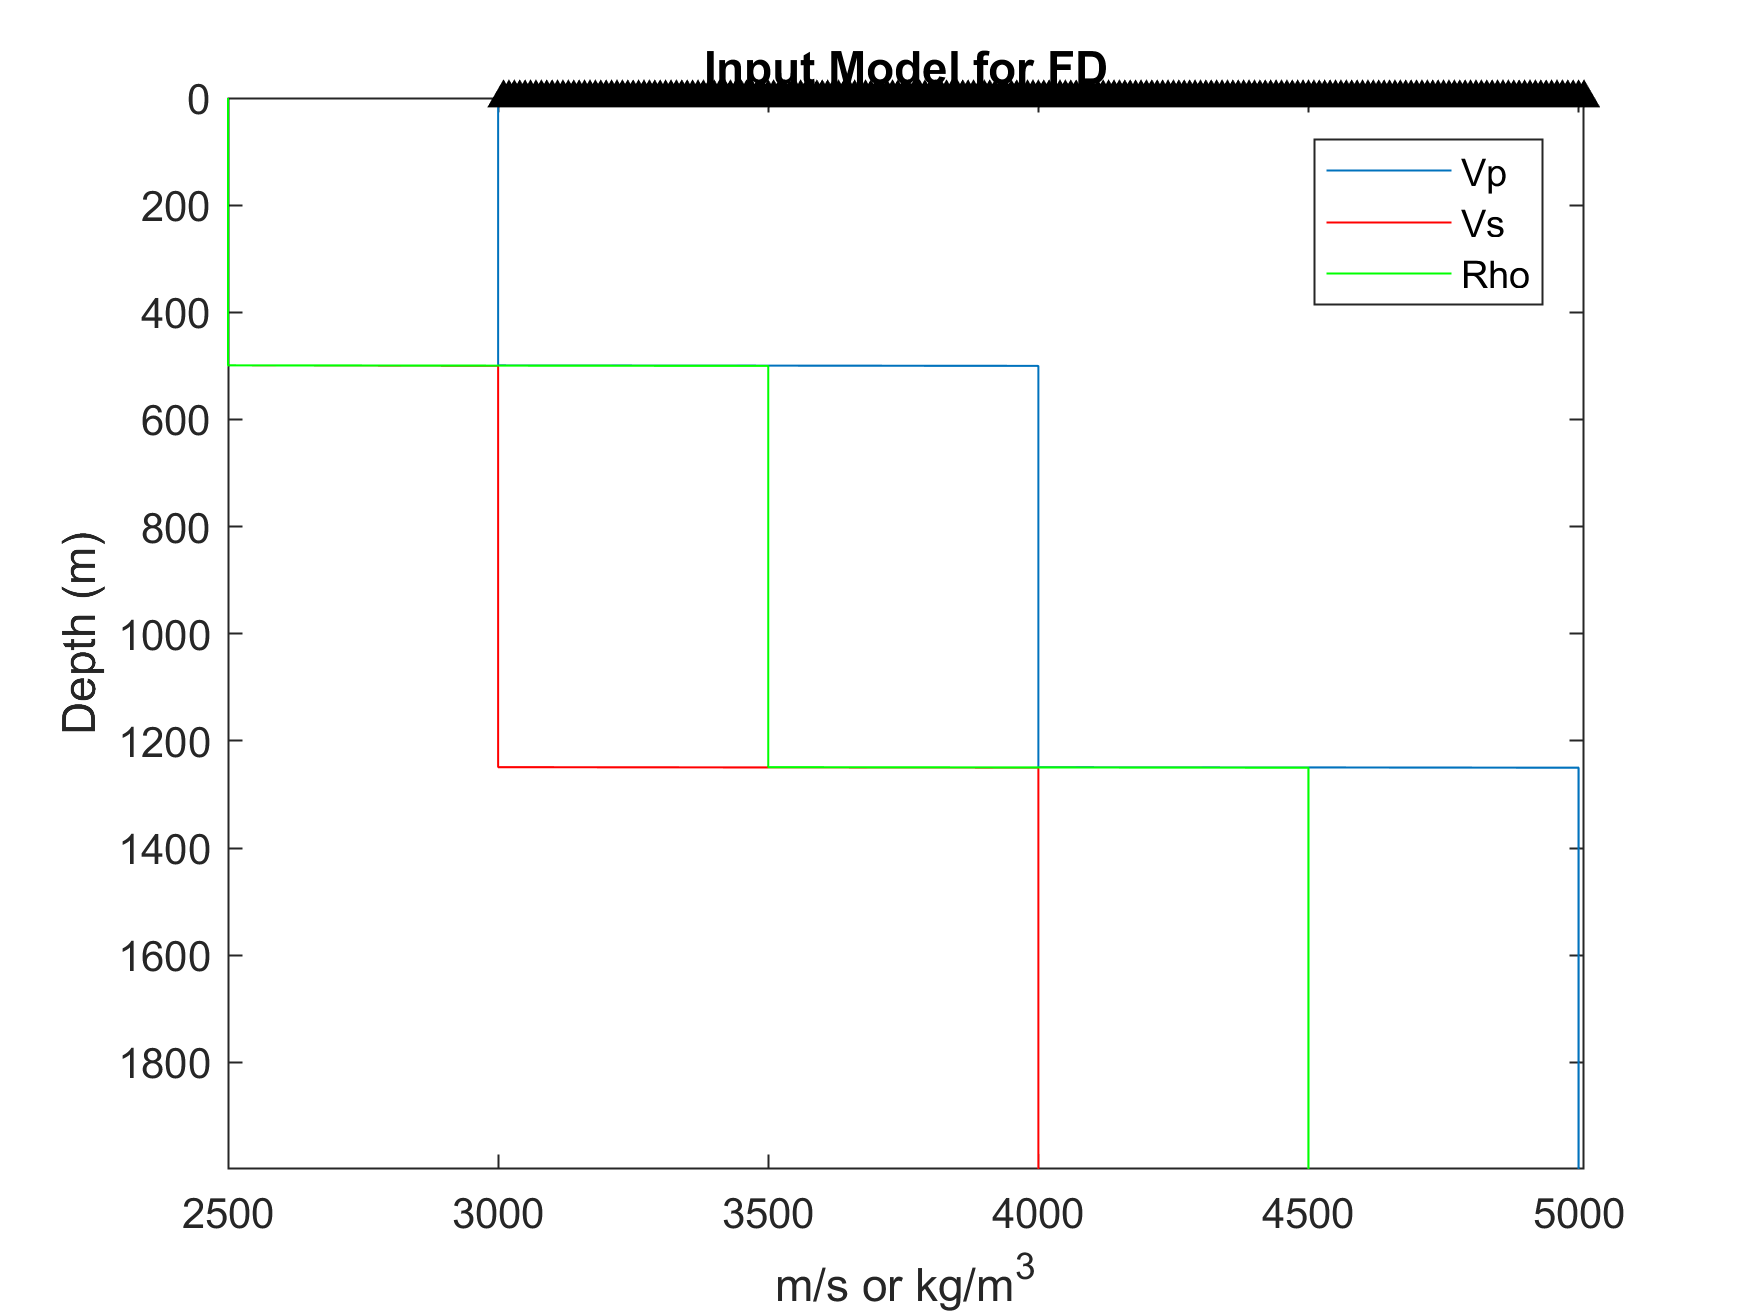
\includegraphics[width=0.8\textwidth]{Figures/FD3InputModel.png}
	\caption[3-layer input test model]{3-layer input model for ray-tracing and finite-difference models}
	\label{fig:3Input}
\end{figure}

\begin{figure}[!htb]
	\centering
	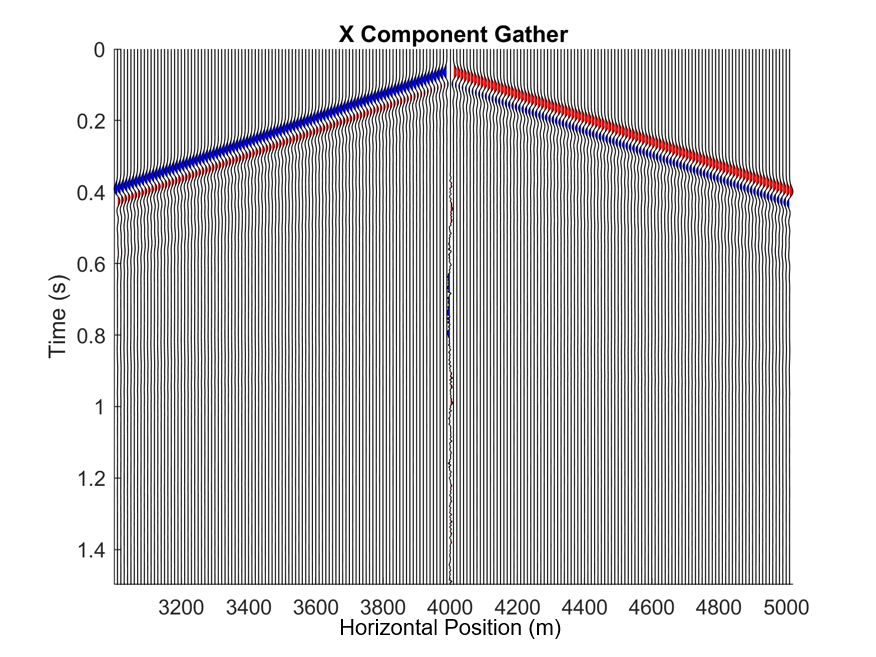
\includegraphics[width=0.8\textwidth]{Figures/FD3XComponentGather.png}
	\caption[Finite-difference 3-layer output gather]{Uncorrected P-Sv Output gather from the finite-difference tool}
	\label{fig:FD3XGather}
\end{figure}

	The first processing step is to reformat the gather by removing all of the data on the left side of the shot, as seen in figure \ref{fig:FD3RefGather}. This was done as the polarities are flipped on the left and right sides of the shot and when they are stacked they would cancel each other out, creating a synthetic with an amplitude of zero. An alternate method is to only place geophones on the right side of the model.
	
\begin{figure}[!htb]
	\centering
	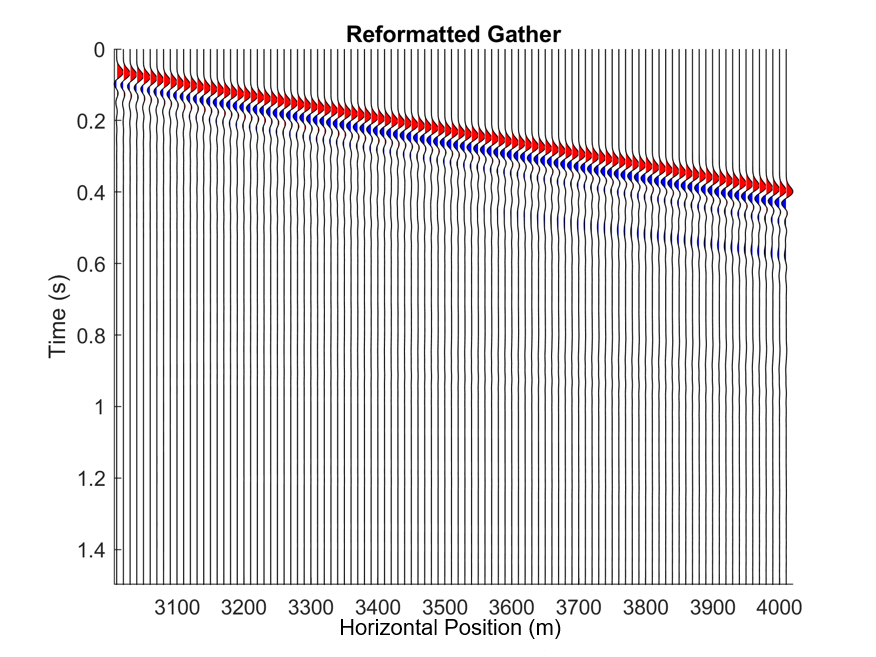
\includegraphics[width=0.8\textwidth]{Figures/FD3ReformattedGather.png}
	\caption[Finite-difference 3-layer reformatted gather] {Gather with all data to the left of the shot removed}
	\label{fig:FD3RefGather}
\end{figure}
	
	Next, the gather must be gain corrected. In this case, the gain correction was made by applying an automatic gain control (AGC). AGC is a data-dependent form of gain adjustment where each sample is multiplied by a scalar derived from a window of data around the sample. This scalar is found by calculating the RMS amplitude in the time window. The AGC corrected gather can be seen in figure \ref{fig:FD3Gain}.
	
\begin{figure}[!htb]
	\centering
	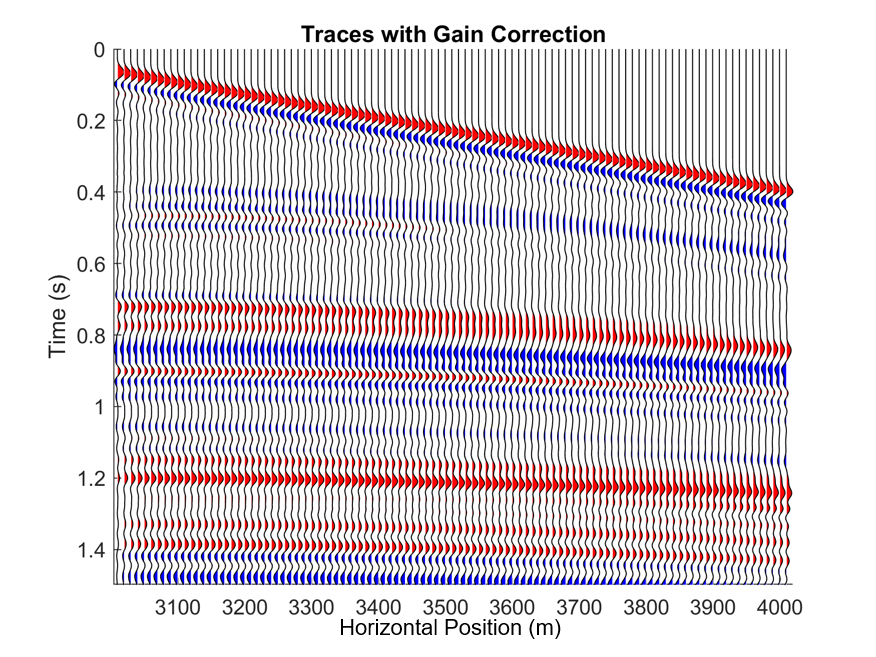
\includegraphics[width=0.8\textwidth]{Figures/FD3TraceswithGainCorrection.png}
	\caption[Finite-difference 3-layer gain correction]{Gain corrected gather}
	\label{fig:FD3Gain}
\end{figure}
	
	The next processing step is to correct the velocities of the gather by using normal moveout (NMO). This is done to flatten the hyperbolic reflections that are visible in the gather. First, a velocity analysis must be done on the data. This can be done in several ways, but the velocity spectrum analysis is the method that will be used to determine these velocities as it maps the time-space data of a single CMP gather on a velocity spectrum plane. \cite{mousa2011} explained the steps used in this analysis. The outputs from this are the stacking times and velocities which are then used in the NMO correction.
	
	The NMO correction applies the picked stacking velocities to the CMP traces and corrects all the non-zero offset traveltimes to prepare the data for stacking. In our use case, there are only horizontal layers so the time-distance curve is a hyperbola given by:
\begin{equation}
	\label{eqn:hyperbola}
	t^2(x)=t_0^2+\frac{x^2}{v^2}
\end{equation}

\noindent where $t(x)$ is the two-way travel time, $t_0$ is the two-way zero offset travel time, $x$ is the offset and $v$ is the layer velocity. The normal moveout, $\Delta t_{NMO}(x)$, is the time difference between the two-way traveltime and the zero-offset travel time at each offset:
\begin{equation}
	\label{eqn:dtNMO}
	\Delta t_{NMO}(x)=t(x)-t_0
\end{equation}

\noindent It can then be shown that the NMO-correction for a horizontally layered system at small offsets is:
\begin{equation}
	\label{eqn:NMOcorr}
	t_{NMO}(x)\approx \frac{x^2}{2t_0 v^2}
\end{equation}

\noindent Equation \ref{eqn:NMOcorr} implies that if the proper velocity is used, the reflection will appear flat. If a velocity that is too large is used, the event will be under-corrected and result in a concave down pattern or "frowns". If a velocity that is too small is used, the event will be over-corrected and result in a concave up pattern or "smiles". NMO corrections can result in stretching of the trace occurring. When this happens, that part of the trace must be muted, however, in this case, we are only using small offsets, so this effect can be ignored. The results from the NMO correction can be seen in \ref{fig:FD3NMO}.

\begin{figure}[!htb]
	\centering
	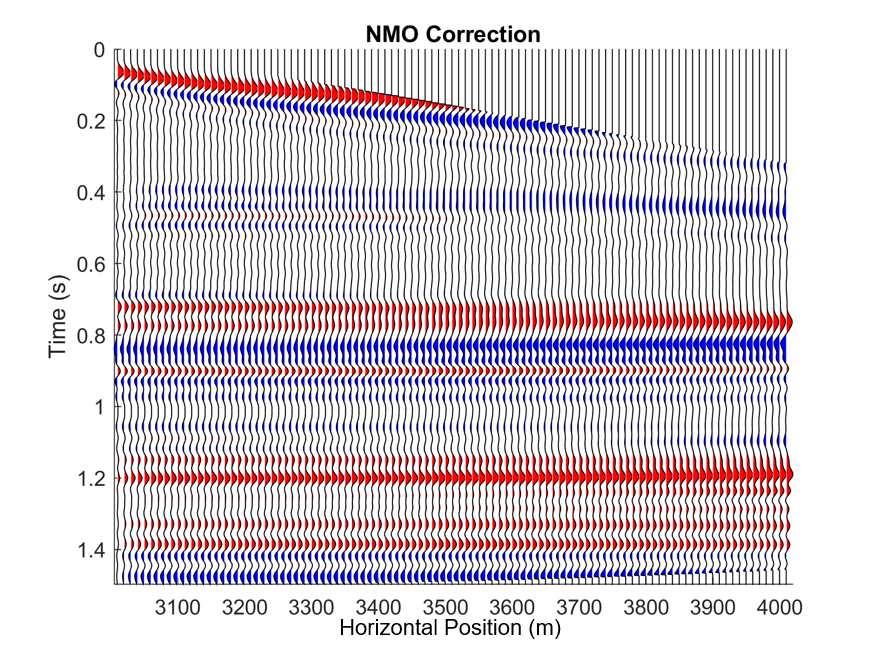
\includegraphics[width=0.8\textwidth]{Figures/FD3NMOCorrection.png}
	\caption[Finite-difference 3-layer NMO correction]{NMO corrected gather. Note that in this figure, the reflection amplitudes vary at offset. This is simply an artifact used in the plotting algorithm and is not present in the real data.}
	\label{fig:FD3NMO}
\end{figure}	
	
	Figure \ref{fig:FD3Stacked} shows the final stacked trace. This is the synthetic seismogram for this dataset. Typically, stacking is applied in order to increase the signal-to-noise ratio, however, in this case, it is done to generate a 1D trace to represent the synthetic for the well. Once the velocities have been flattened, stacking can be done by summing the traces together. The amplitudes can be either summed or averaged. Figure \ref{fig:FD3StackedSeveral} shows several repeated seismograms placed next to each other. This is done to allow for easier interpretations. 

\begin{figure}[!htb]
	\centering
	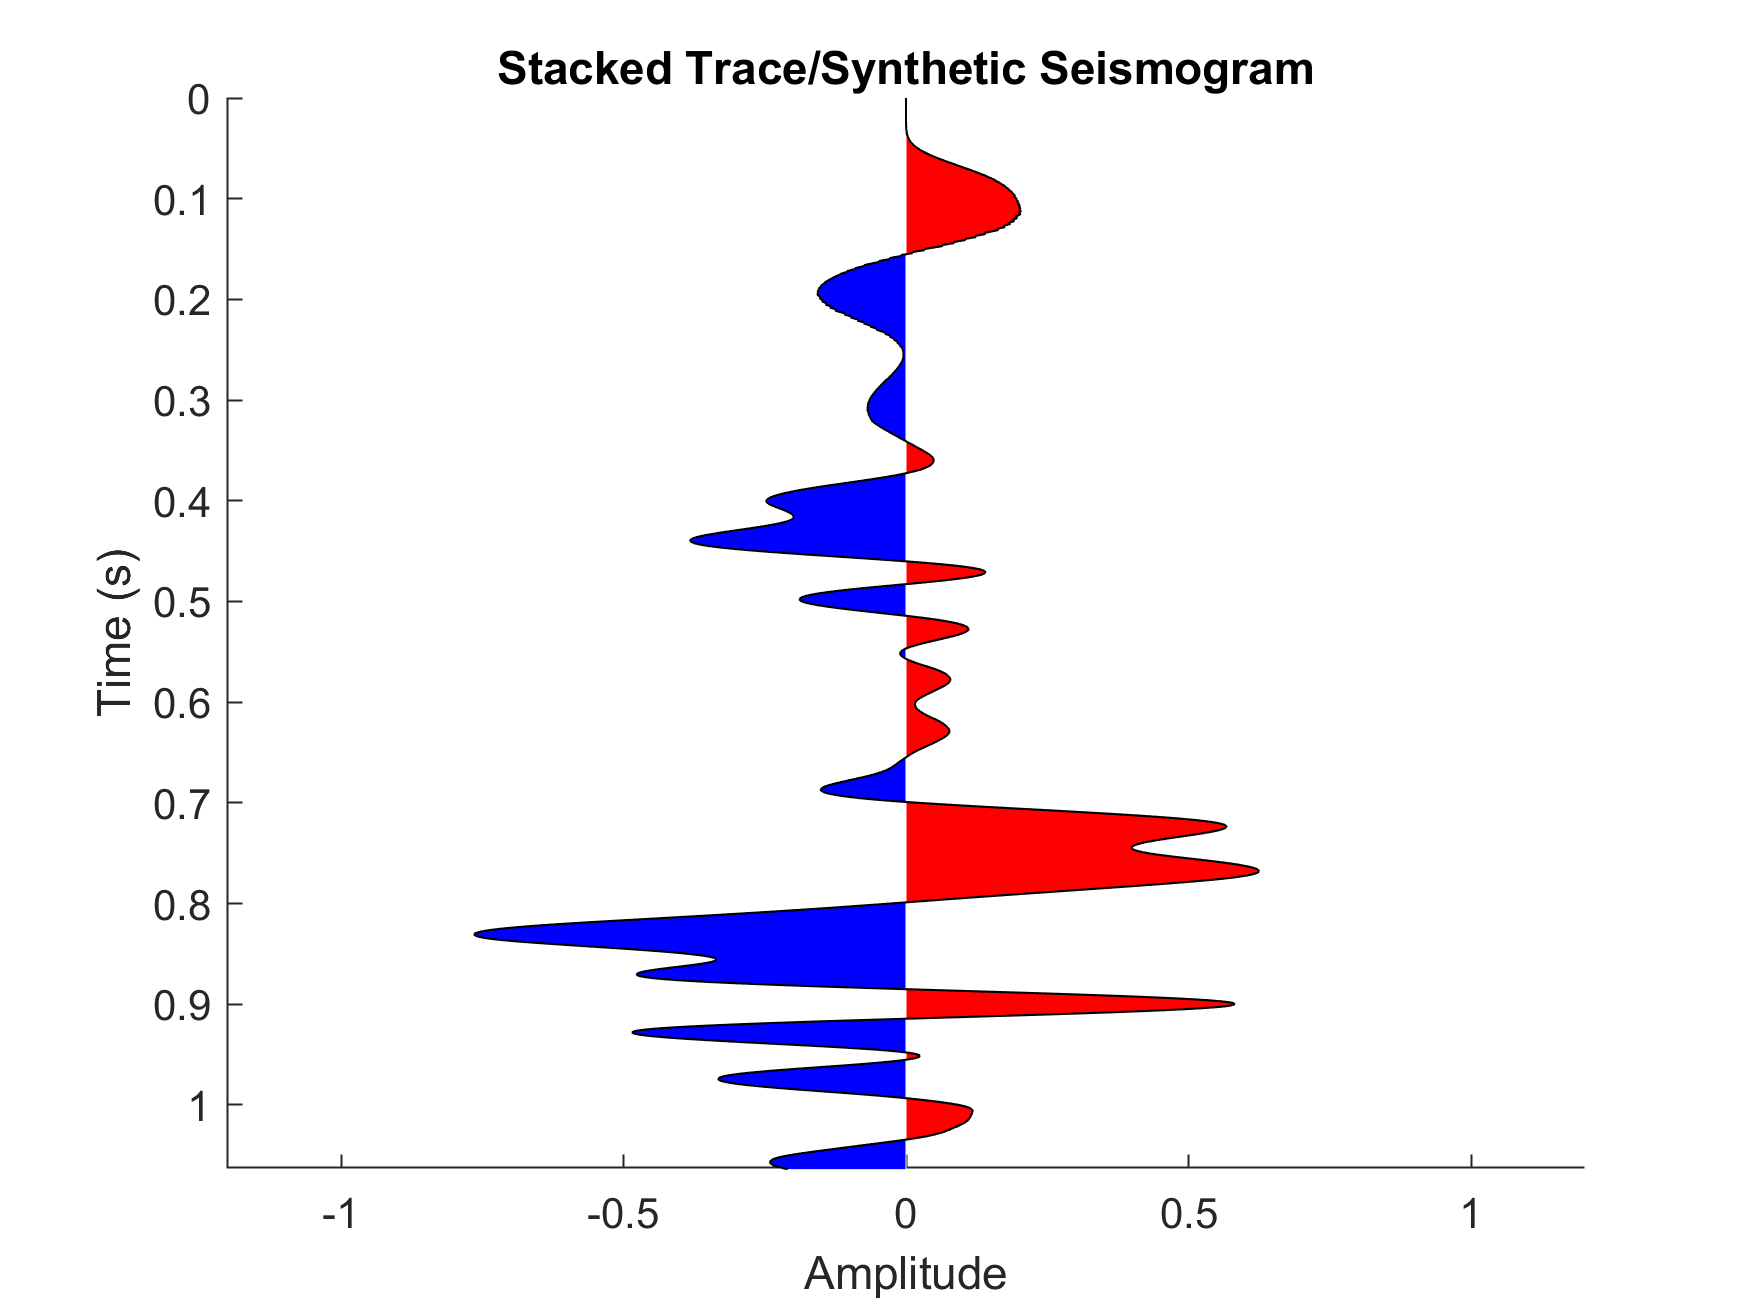
\includegraphics[width=0.8\textwidth]{Figures/FD3StackedTrace.png}
	\caption[Finite-difference 3-layer synthetic seismogram]{Stacked trace and synthetic seismogram}
	\label{fig:FD3Stacked}
\end{figure}

\begin{figure}[!htb]
	\centering
	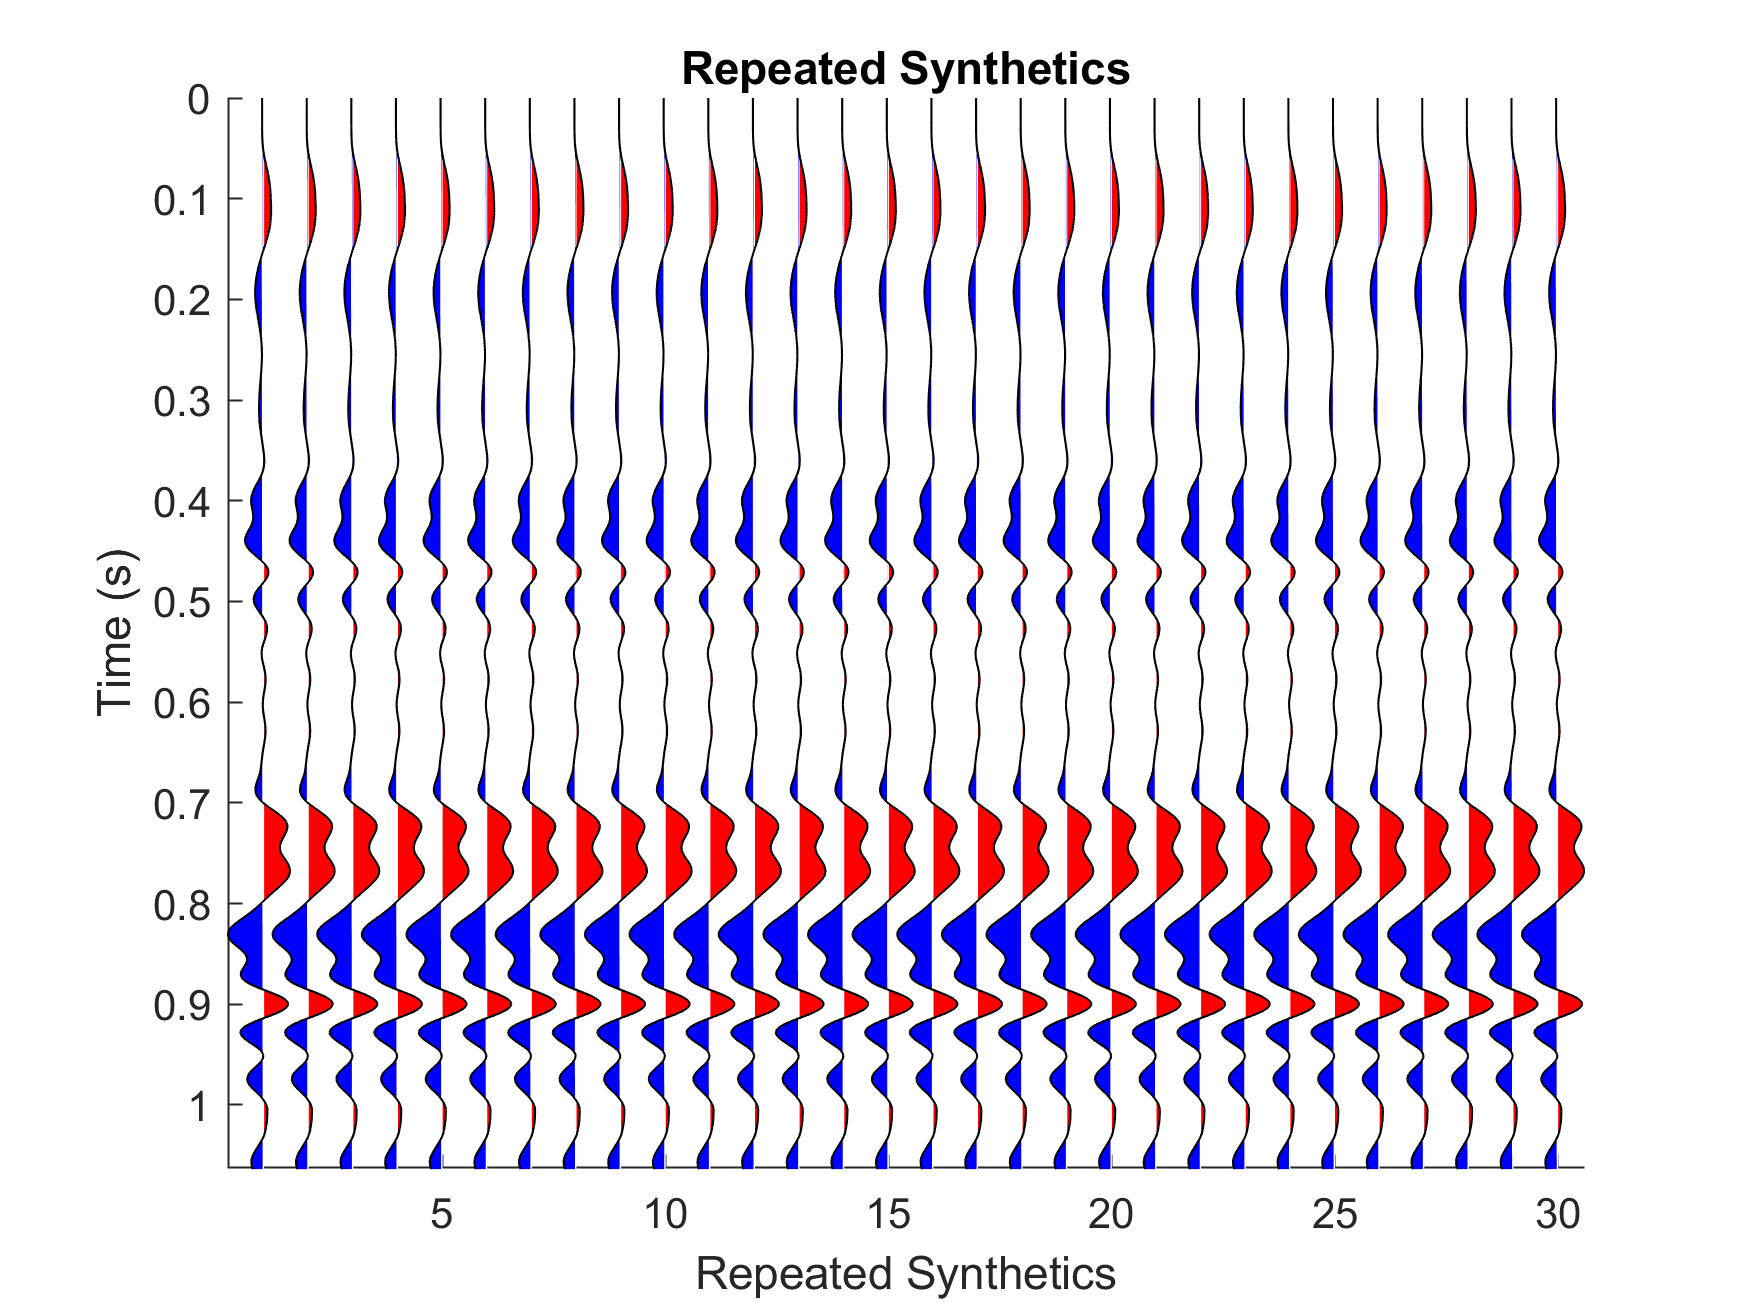
\includegraphics[width=0.8\textwidth]{Figures/FD3SeveralSynthetics.png}
	\caption[Finite-difference 3-layer several synthetic seismograms]{Several seismograms repeated to allow for easier interpretations}
	\label{fig:FD3StackedSeveral}
\end{figure}
	
	The input source wavelet can be adjusted so that the seismogram matches the seismic and to smooth the events. The synthetic can then be overlain with the seismic data and then stretched and squeezed to generate a time-depth-relationship for that well. Once this relationship has been discovered, other well information, such as well logs and tops, can be overlain onto the seismic data as well.
	
	Figure \ref{fig:FD3} illustrates a snapshot of the wave propagation through the synthetic 2D model. This model was $8000 m$ wide and $2000 m$ deep, with a grid spacing of $10 m$. The maximum time was $1.5 s$, with a time step of $0.001 s$. The input wavelet (figure \ref{fig:3Wavelet})  was generated by applying a tenth-order Butterworth filter to an impulse with a high cut frequency of $20 Hz$. This created a minimum phase wavelet that is rich with low frequencies. On a dual-core CPU with a clock speed of $2.7 GHz$, the model and processing corrections took approximately 15 minutes to run, illustrating that this is a very computationally expensive method.
	
\begin{figure}[!htb]
	\centering
	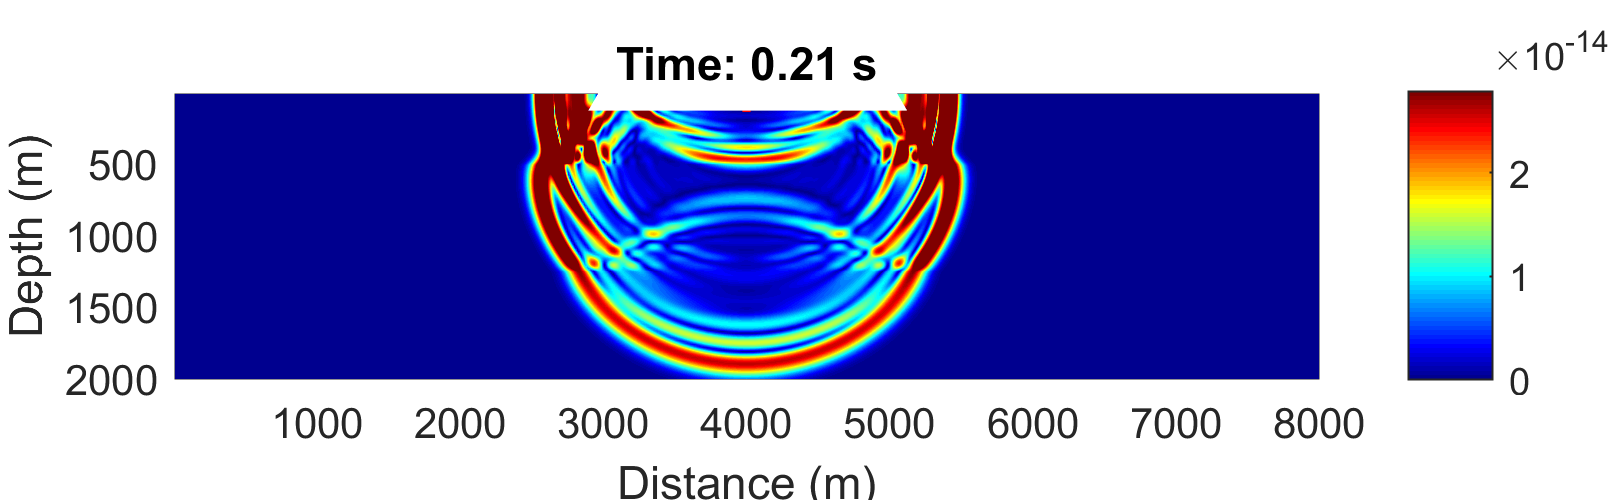
\includegraphics[width=0.9\textwidth]{Figures/FD3Movie_132.png}
	\caption[Finite-difference 3-layer wave propagation]{Finite-difference wave propagation of a 3-layer earth model}
	\label{fig:FD3}
\end{figure}

\begin{figure}[!htb]
	\centering
	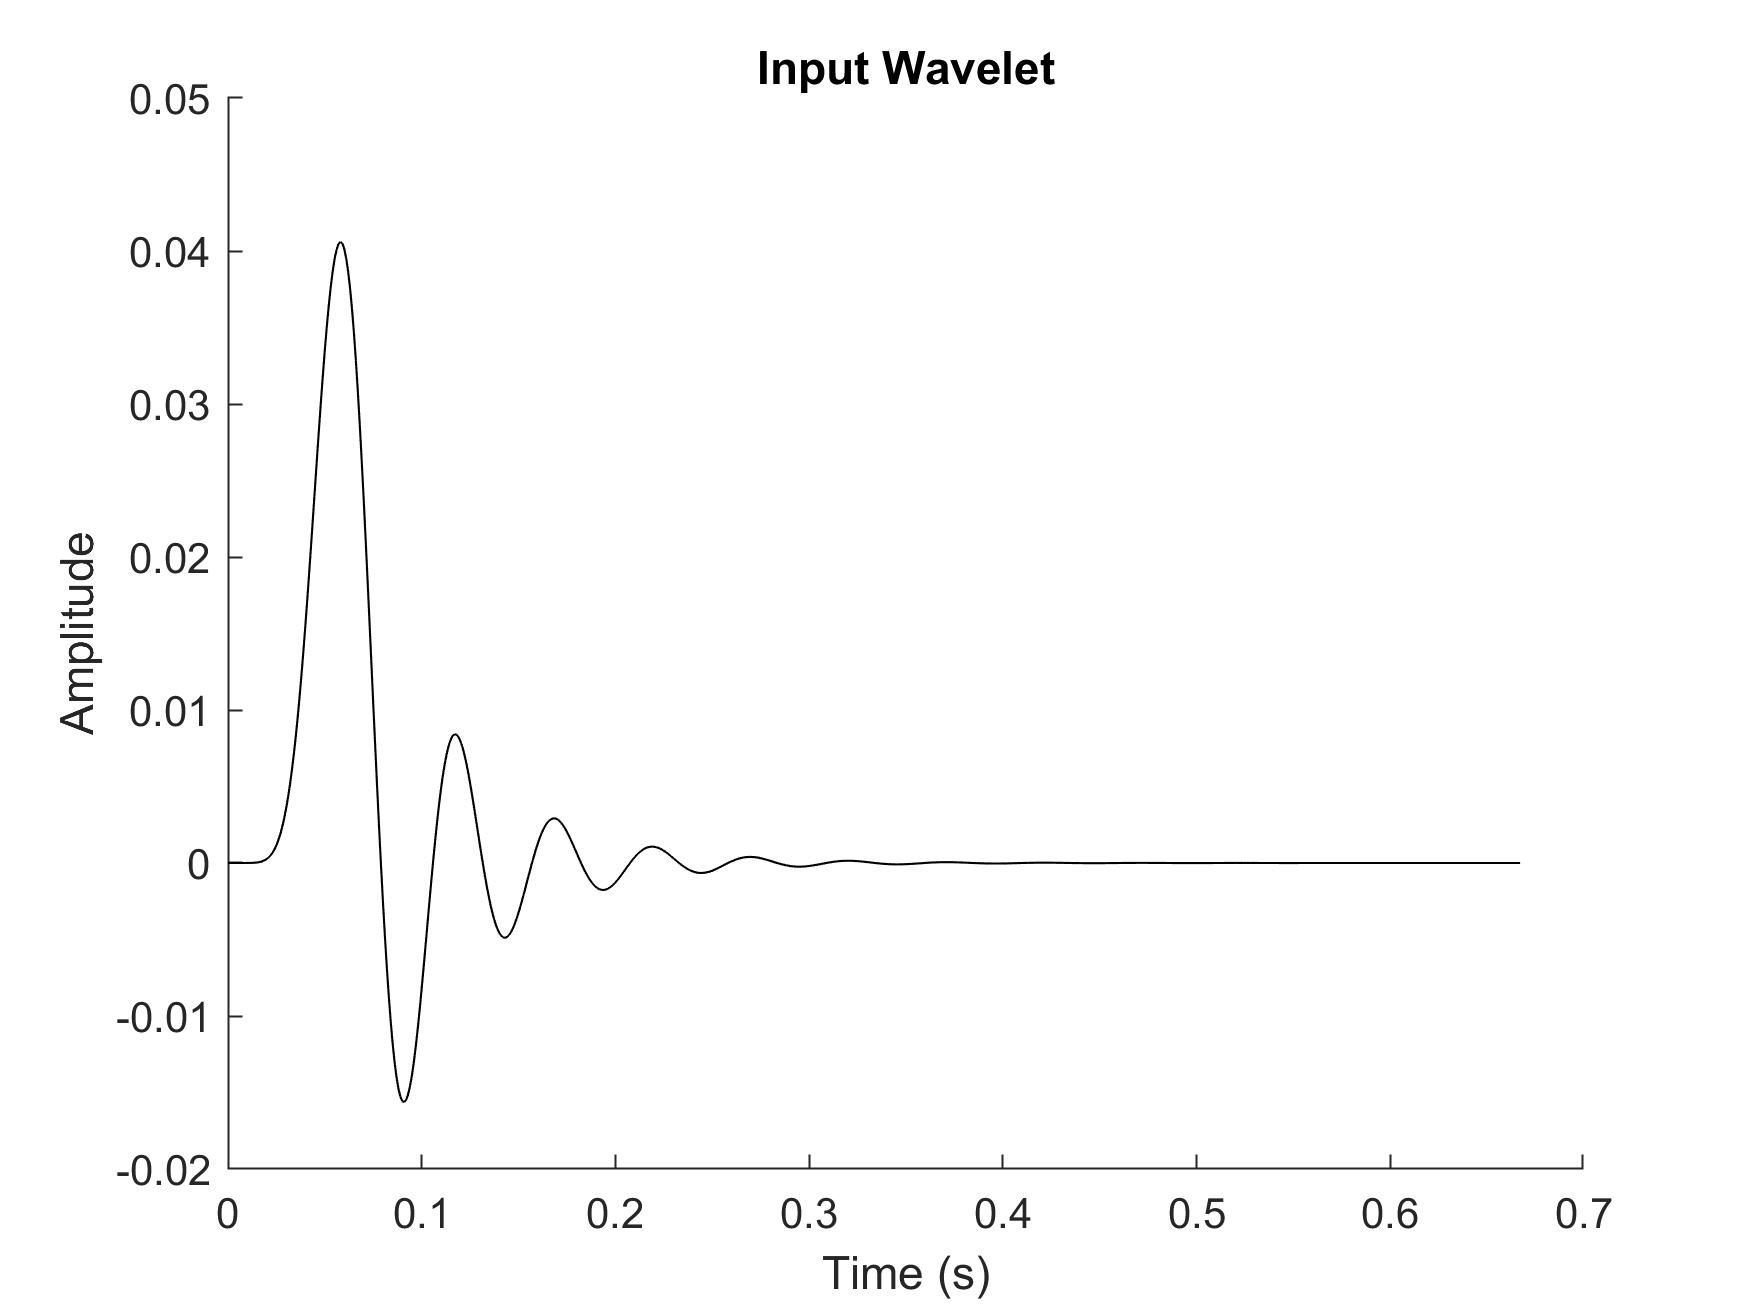
\includegraphics[width=0.8\textwidth]{Figures/FD3InputWavelet.png}
	\caption[Finite-difference source and ray-tracing convolution wavelet]{A low-frequency rich source wavelet for finite-difference methods and the convolutional wavelet for ray-tracing}
	\label{fig:3Wavelet}
\end{figure}

	Finite-difference modelling is a very useful tool to generate synthetic seismograms. This approach accounts direct waves, primary reflected waves, multiple reflected waves, surface waves, head waves, converted waves, diffracted waves and critically refracted waves, making it a very accurate way of modelling the earth. In some cases, however, not all of these waves are desired in the synthetic generation. The high computational burden must also be considered. 

\FloatBarrier
\subsection{Ray-Tracing}
	
	Rays are defined as the normal to the wavefront and they point out in the direction of wave propagation and as such, they are a high-frequency approximation of the wave propagation \citep{Hanyga1995}. Ray-tracing methods are considerably faster than solving the wave equation with finite-differences, however, they contain simplifications that can make them less precise than wave equation solutions.
		
	Ray-tracing techniques utilize a similar earth model to that of the finite-difference method. By using P-wave, S-wave and density well logs, a horizontal layer earth model is created, using a specified layer thickness ($\Delta z$). A ray is sent into the model at a chosen incidence angle the ray propagation is traced using Snell's Law: 

\begin{equation}
	\label{eqn:Snell}
	\frac{sin(\theta_1)}{sin(\theta_2)}=\frac{V_1}{V_2}=p
\end{equation}	
	
\noindent where $p$ is the ray parameter, $\theta_1$ and $V_1$ are the angles of incidence and velocity of the upper layer and $\theta_2$ and $V_2$ can be either the transmission angle and velocity of the lower layer or the reflection angle and converted wave velocity of the upper layer. For each layer ($i$), the horizontal distance travelled ($X_i$) and the travel time ($t_i$) can be found using equations \ref{eqn:xdist} and \ref{eqn:tt} respectively, so long as the angle of incidence of the layer ($\theta_i$) is known.
	

\begin{equation}
	\label{eqn:xdist}
	X_i=tan(\theta_i) \cdot \Delta z
\end{equation}
\begin{equation}
	\label{eqn:tt}
	t_i=\frac{\Delta z}{cos(\theta_i) \cdot V_i}
\end{equation}

	The incidence angles in the first layer are cycled through at a specified interval, creating a fan of rays. Figure \ref{fig:RT3AllPath} shows the results of ray-tracing using the same 3-layer input earth model as the finite-difference method (figure \ref{fig:3Input}), divided into 13 different layers with ray input angles every 10\degree. Each layer uses averages of the input log values at that layer. 
	
\begin{figure}[!htb]
	\centering
	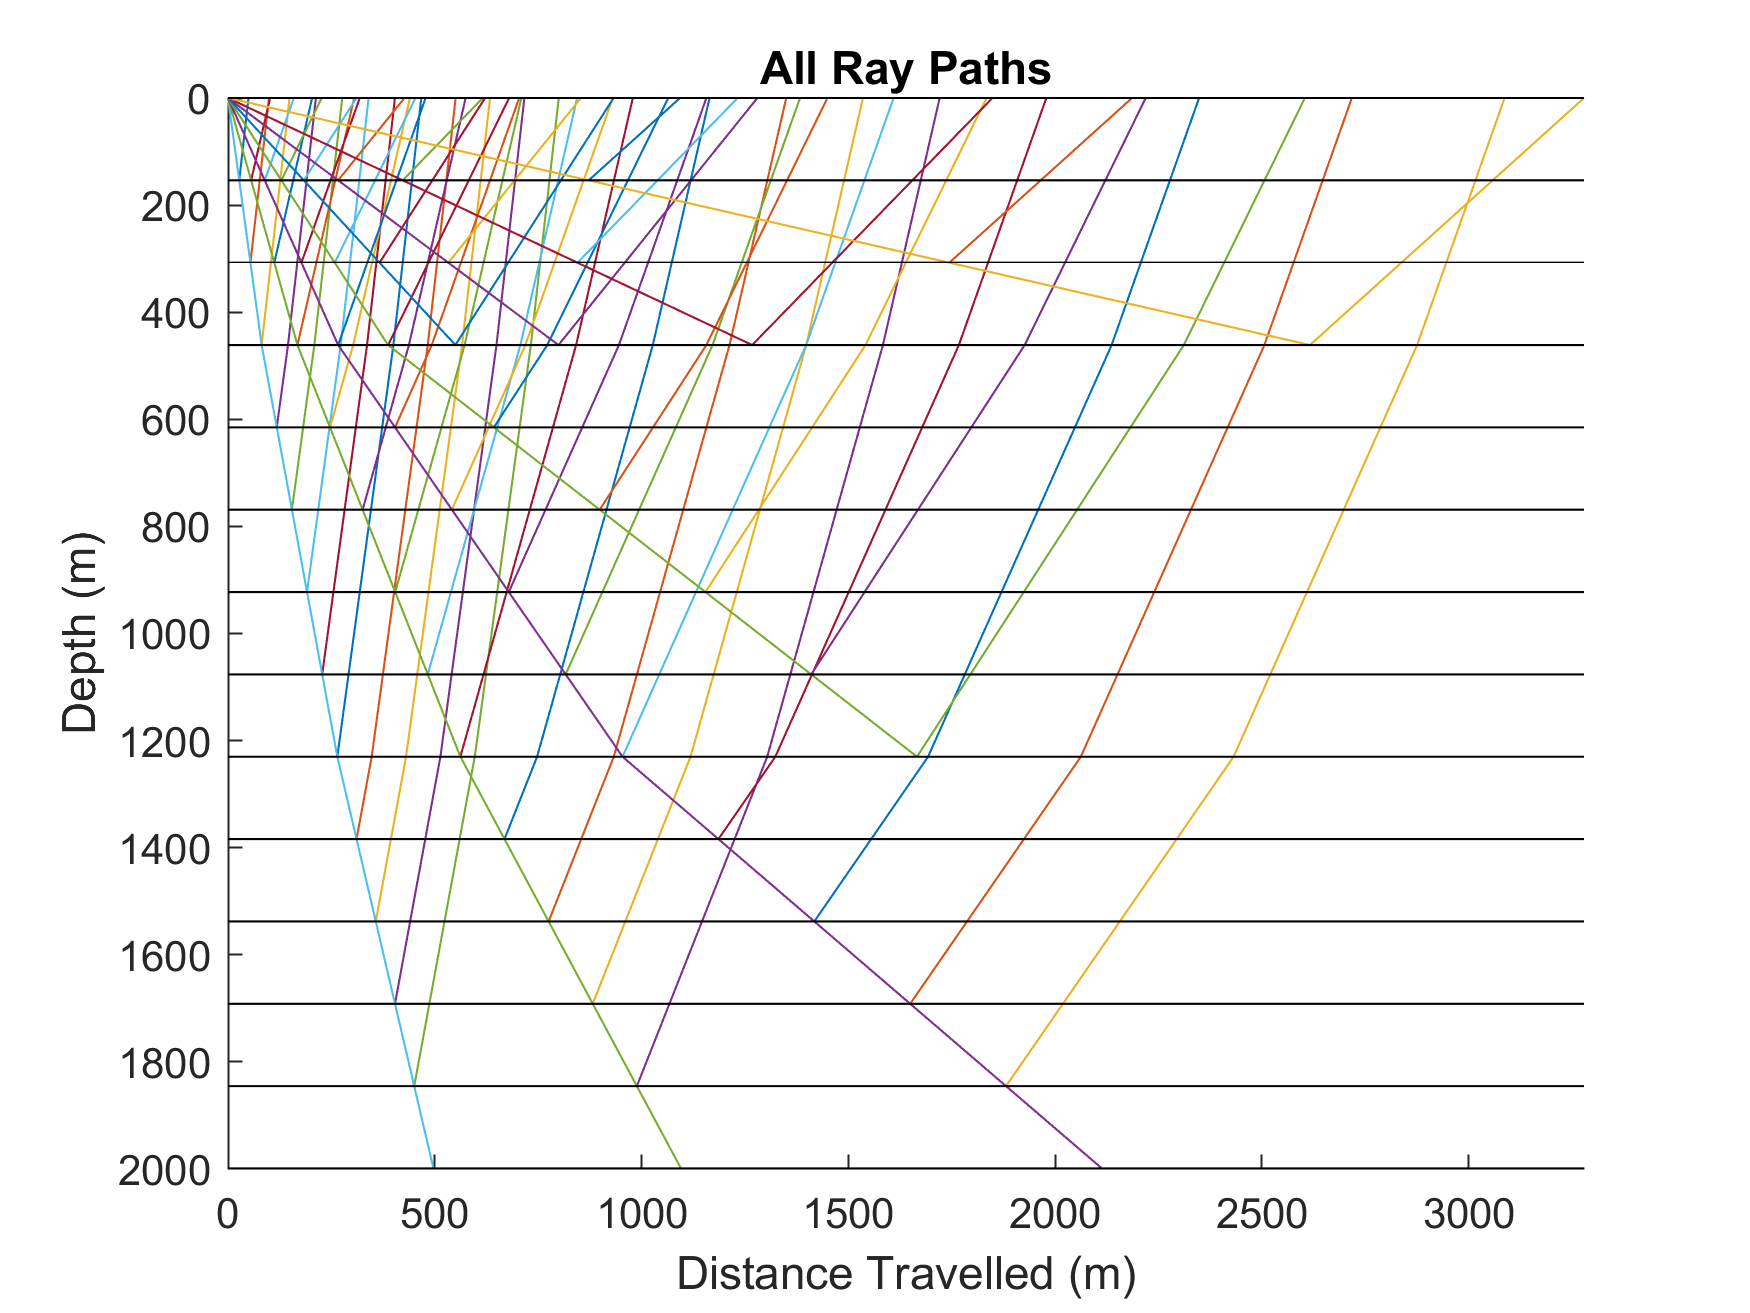
\includegraphics[width=0.8\textwidth]{Figures/RT3AllRayPath.png}
	\caption[Ray-tracing 3-layer ray fan]{P-Sv ray-tracing using a 3-layer input earth model, divided into 13 layers with input angles every 10\degree. Here, the down-going ray is the P-wave and the up-going ray is the S-wave.}
	\label{fig:RT3AllPath}
\end{figure}

	Next, the total offsets of each reflection are calculated. An input offset (typically the average offset of the seismic survey) is chosen and input angles are interpolated to find the input angle of incidence needed for each layer to reflect to the specified offset, as seen in figure \ref{fig:RT3Interp}. The reflection point of the converted wave is asymptotic to a point as depth increases. Figure \ref{fig:RT3DVA} shows that the angle of incidence decreases exponentially as the layer depth increases.
	
\begin{figure}[!htb]
	\centering
	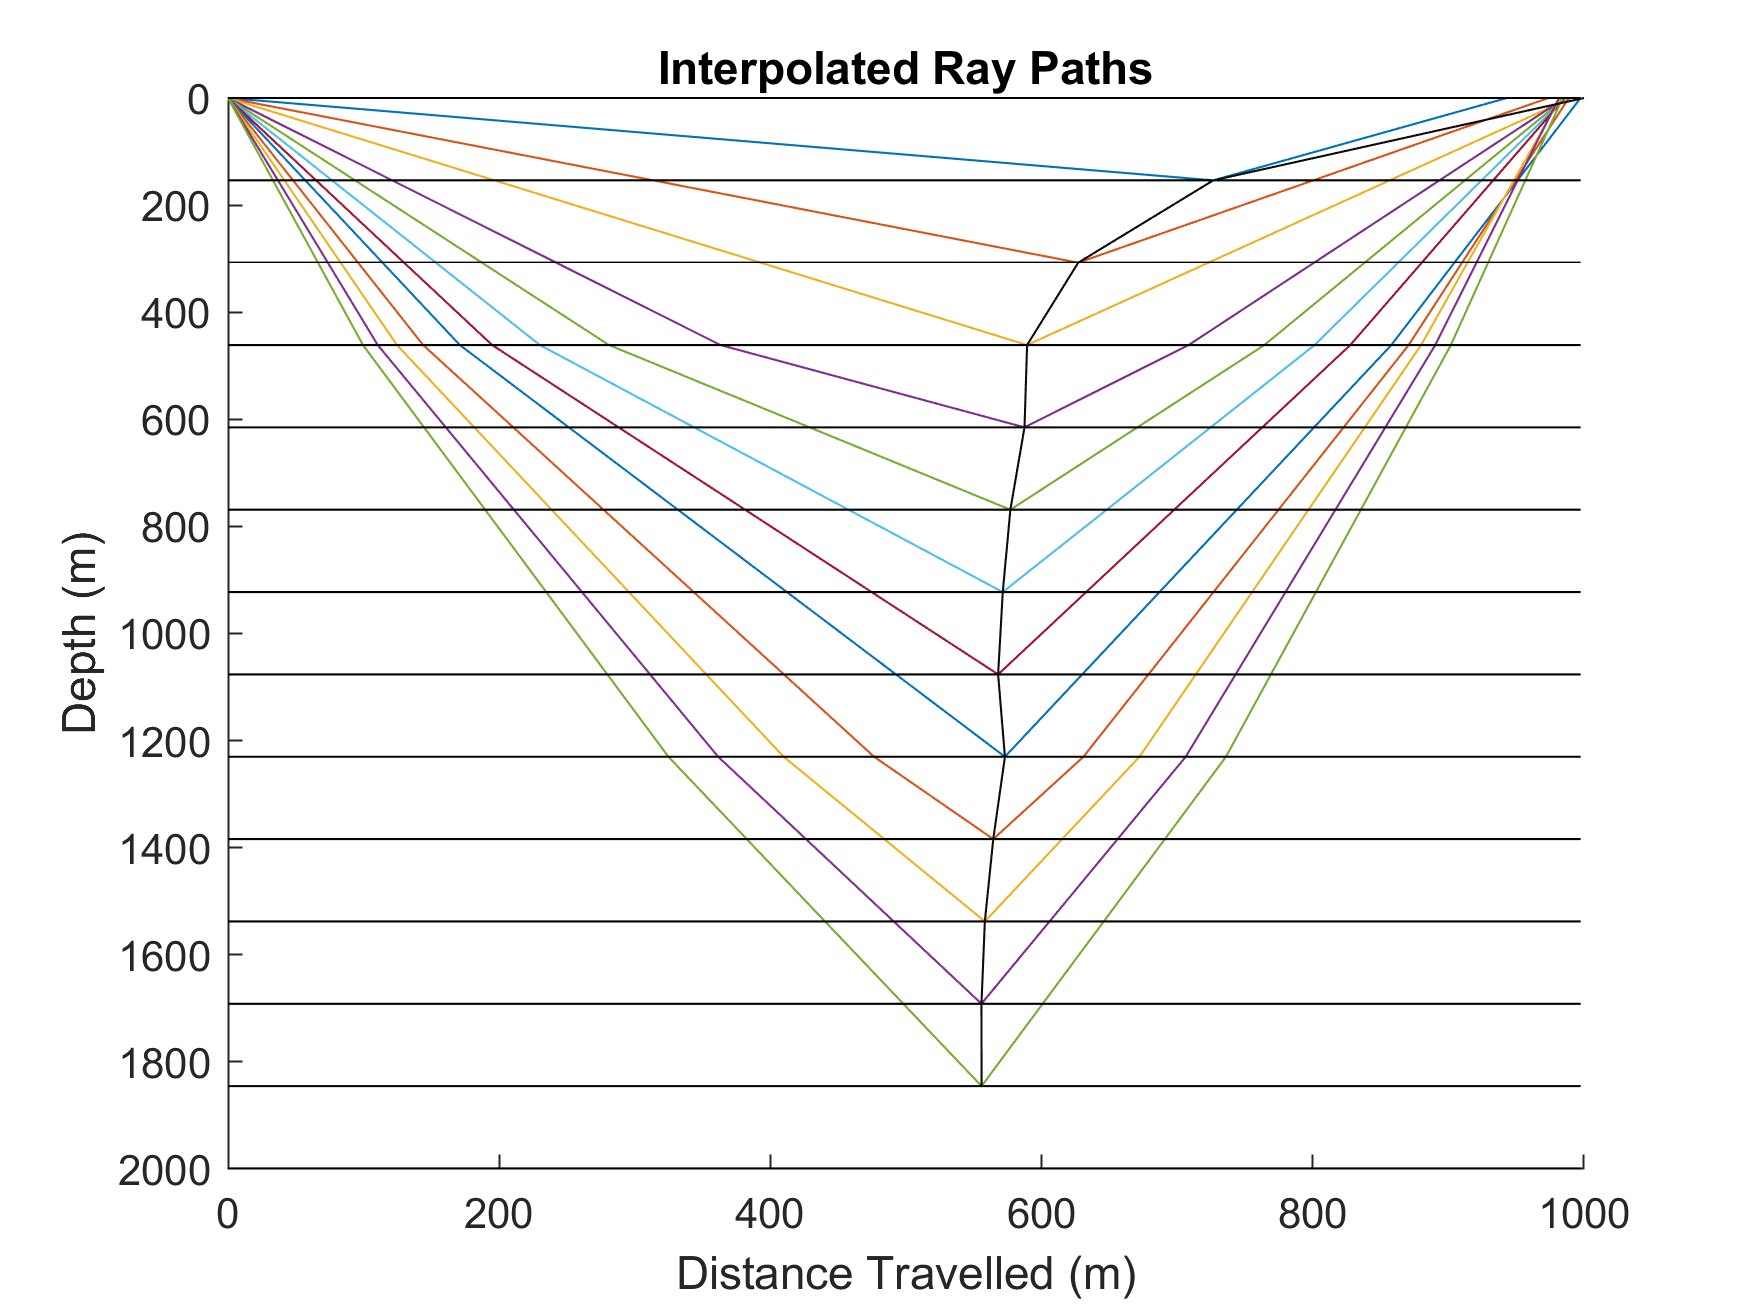
\includegraphics[width=0.8\textwidth]{Figures/RT3InterpolatedRayPath.png}
	\caption[Ray-tracing 3-layer fixed-offset path]{Interpolated ray paths to reach the specified offset. In practice, the specified offset is the average absolute source-receiver distance.}
	\label{fig:RT3Interp}
\end{figure}

\begin{figure}[!htb]
	\centering
	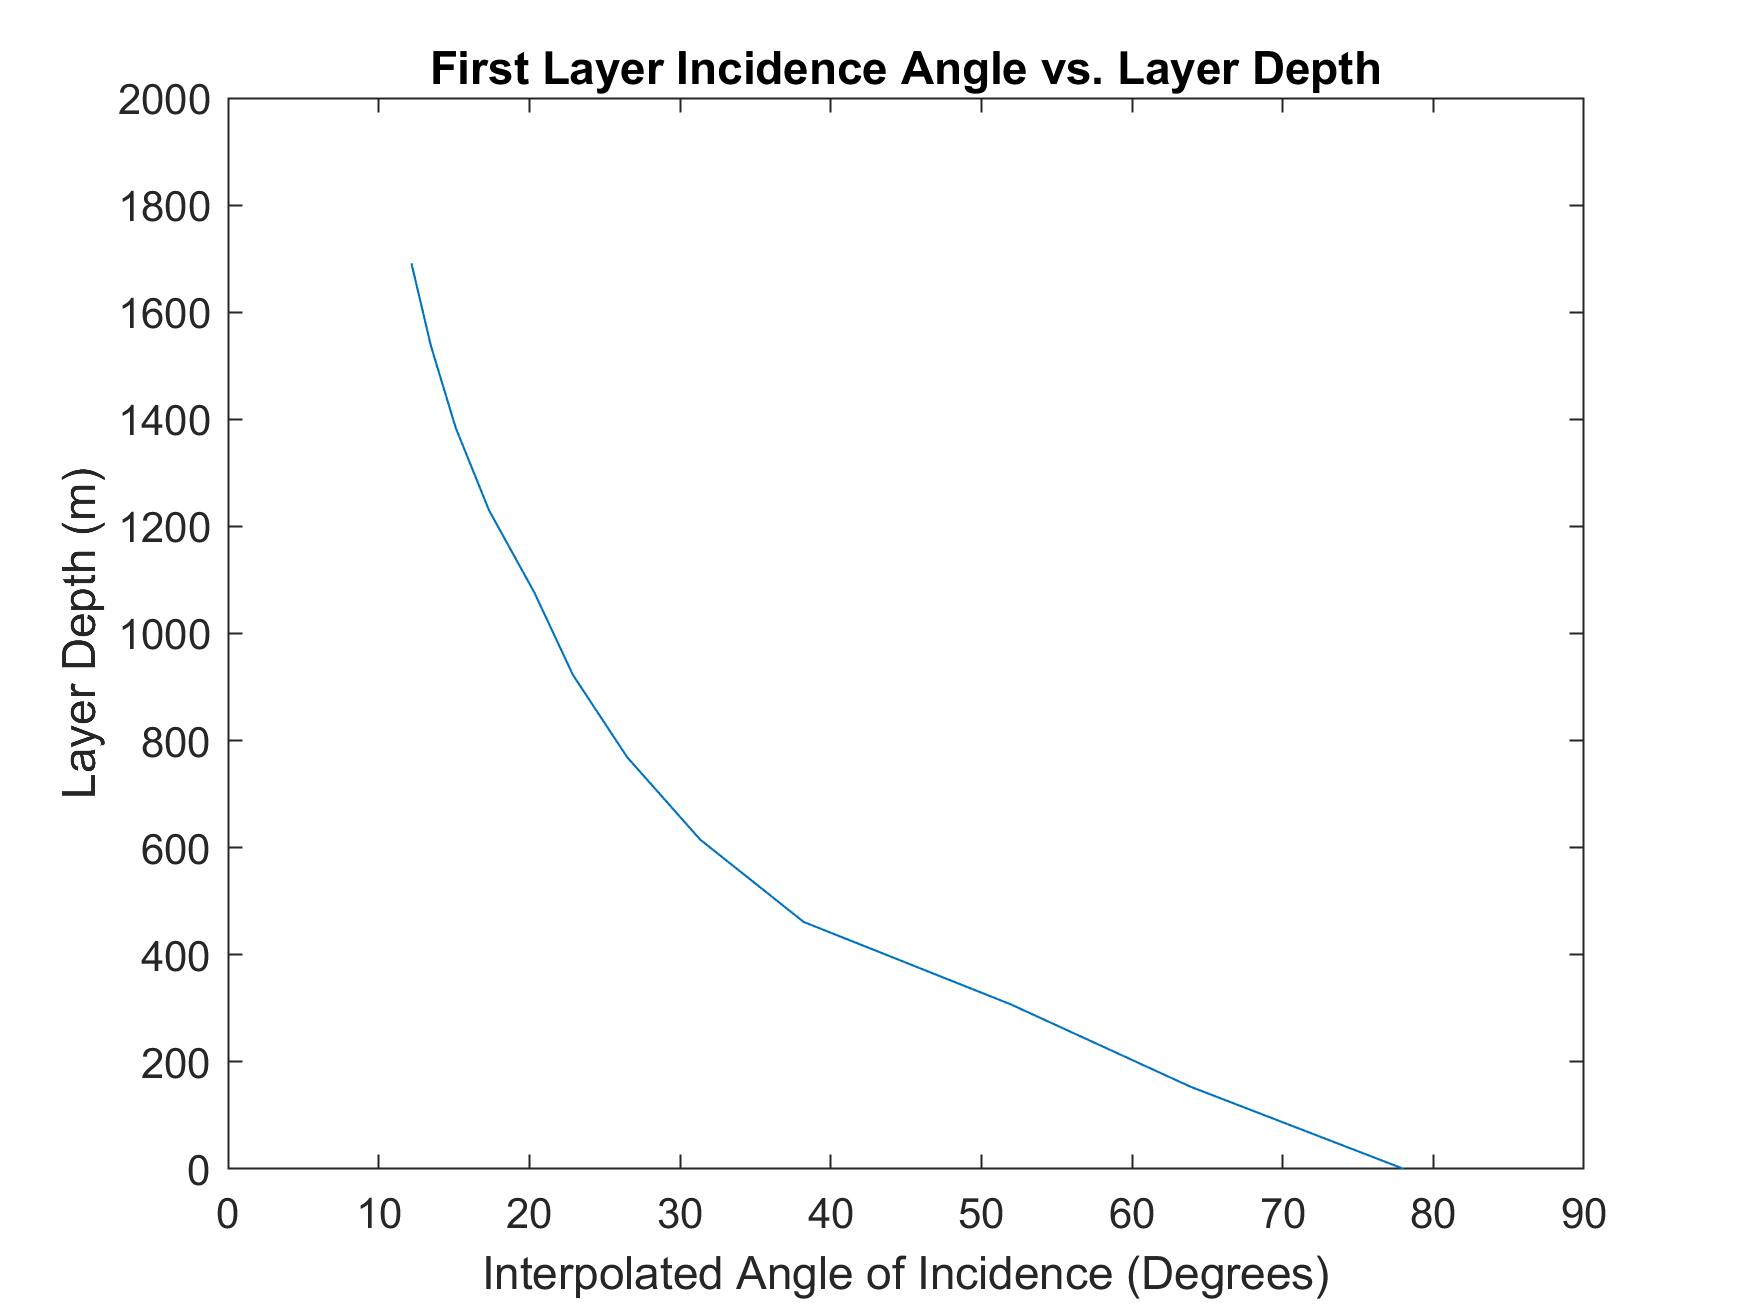
\includegraphics[width=0.8\textwidth]{Figures/RT3AnglevDepth.png}
	\caption[Ray-tracing 3-layer depth-angle plot]{Layer depth as a function of input angle of incidence}
	\label{fig:RT3DVA}
\end{figure}

	The amplitudes are found at each reflection using the Zoeppritz equations \citep{zoeppritz1919}, multiplied by the cosine of the phase to determine polarity and are then matched with each interface's zero-offset time, creating a reflectivity series (Figure \ref{fig:RT3RefSeries}). 
	
\begin{figure}[!htb]
	\centering
	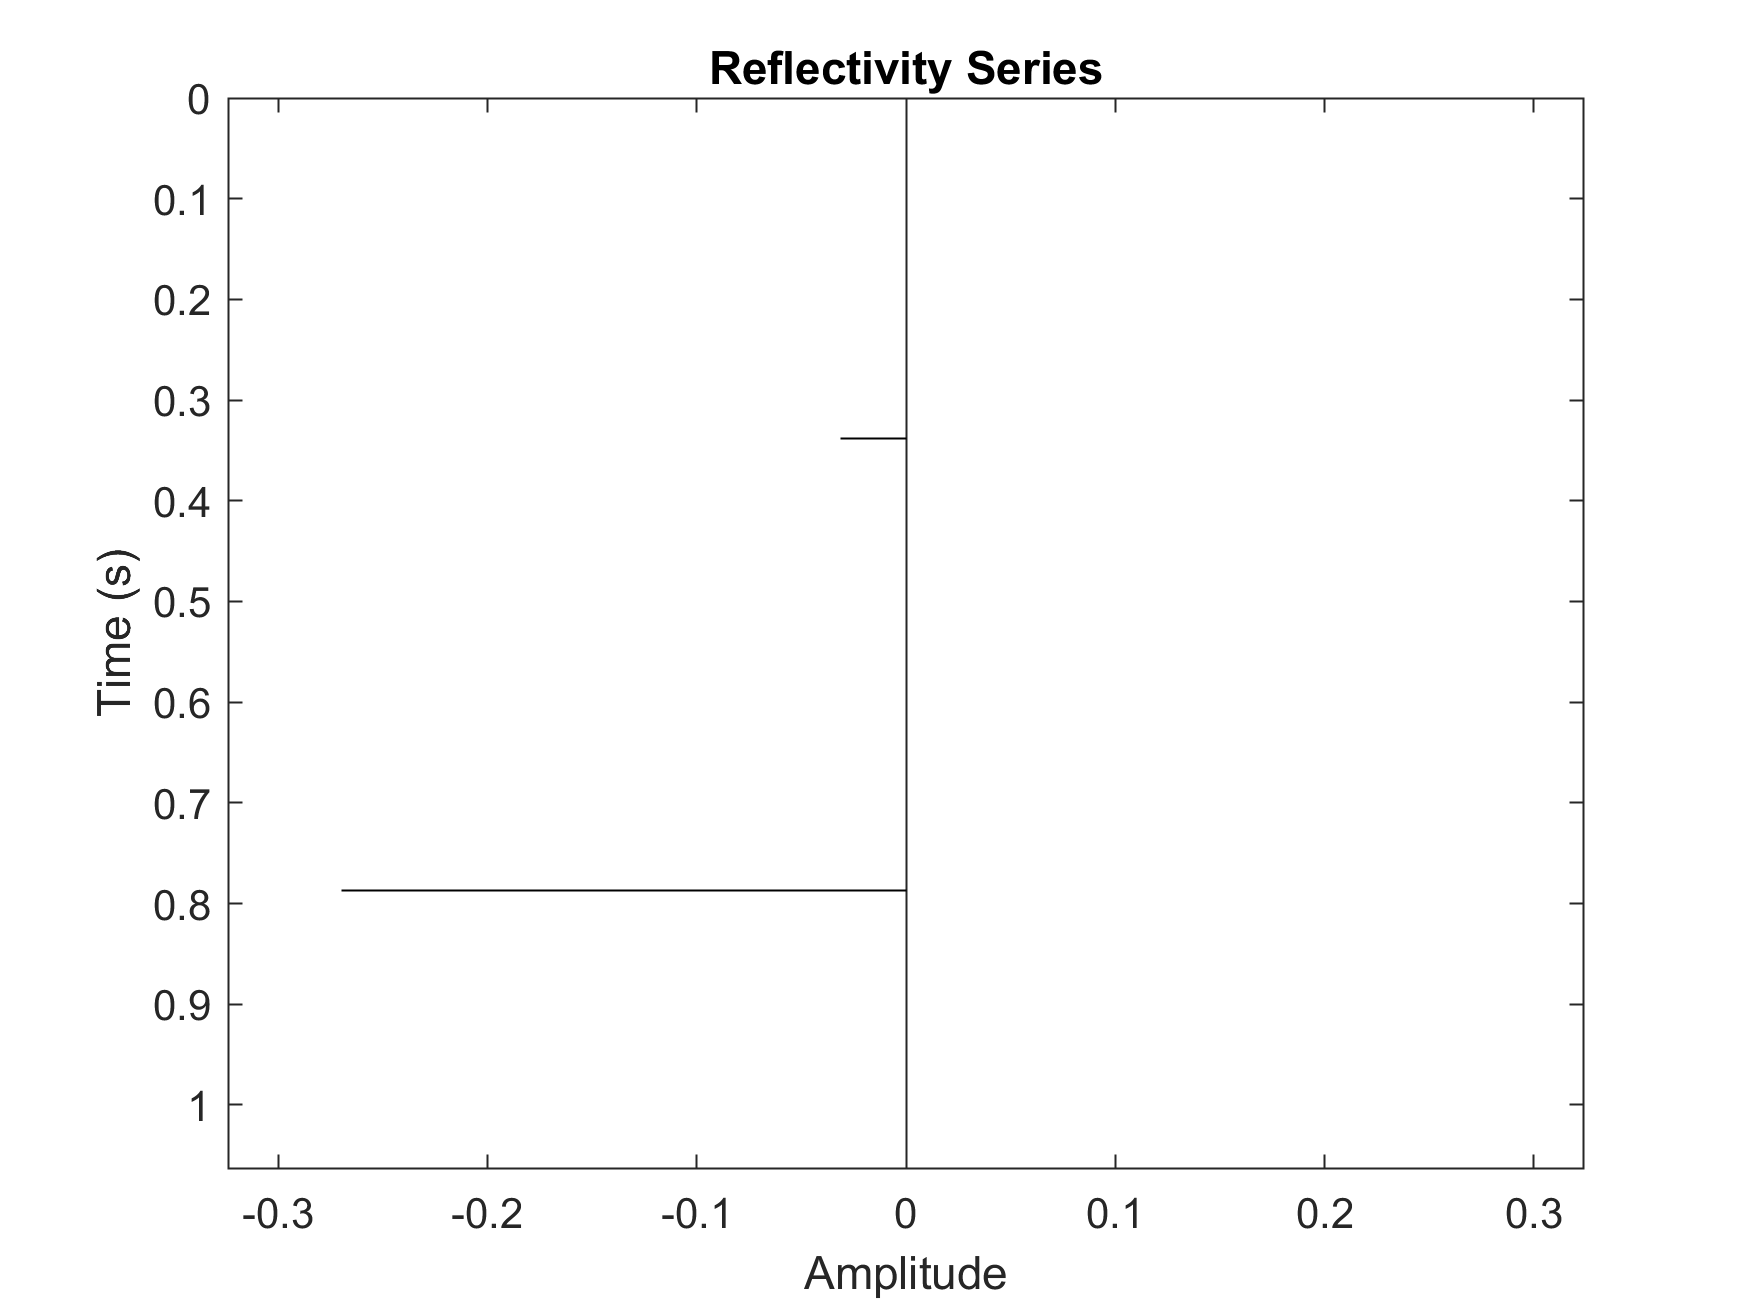
\includegraphics[width=0.8\textwidth]{Figures/RT3ReflectivitySeries.png}
	\caption[Ray-tracing 3-layer reflectivity series]{Reflectivity series of the 3-layer model}
	\label{fig:RT3RefSeries}
\end{figure}

	The reflectivity series is then convolved with an input wavelet using the shift-and-sum method of convolution. Figure \ref{fig:3Wavelet} (above) shows the wavelet used in convolution, a $20Hz$ high cut filtered, minimum phase wavelet. The convolution is made by shifting the wavelet across each sample and summing all of the samples together. When the wavelet is shifted, the amplitudes at the end of the wavelet trace are carried over and start at time equal to zero. 

	Figure \ref{fig:RT3Syn} shows the resulting synthetic seismogram found using ray-tracing methods and figure \ref{fig:RT3Synsev} shows several repeated copies of those synthetics to aid in interpretation. Finally, figure \ref{fig:RT3TimeLog} displays the time-converted well logs, allowing them to be easily correlated with seismic. This model took approximately 9 seconds to run. Note that there are differences between the ray-tracing finite-difference synthetics, and these reasons will be explored in the next chapter.

\begin{figure}[!htb]
	\centering
	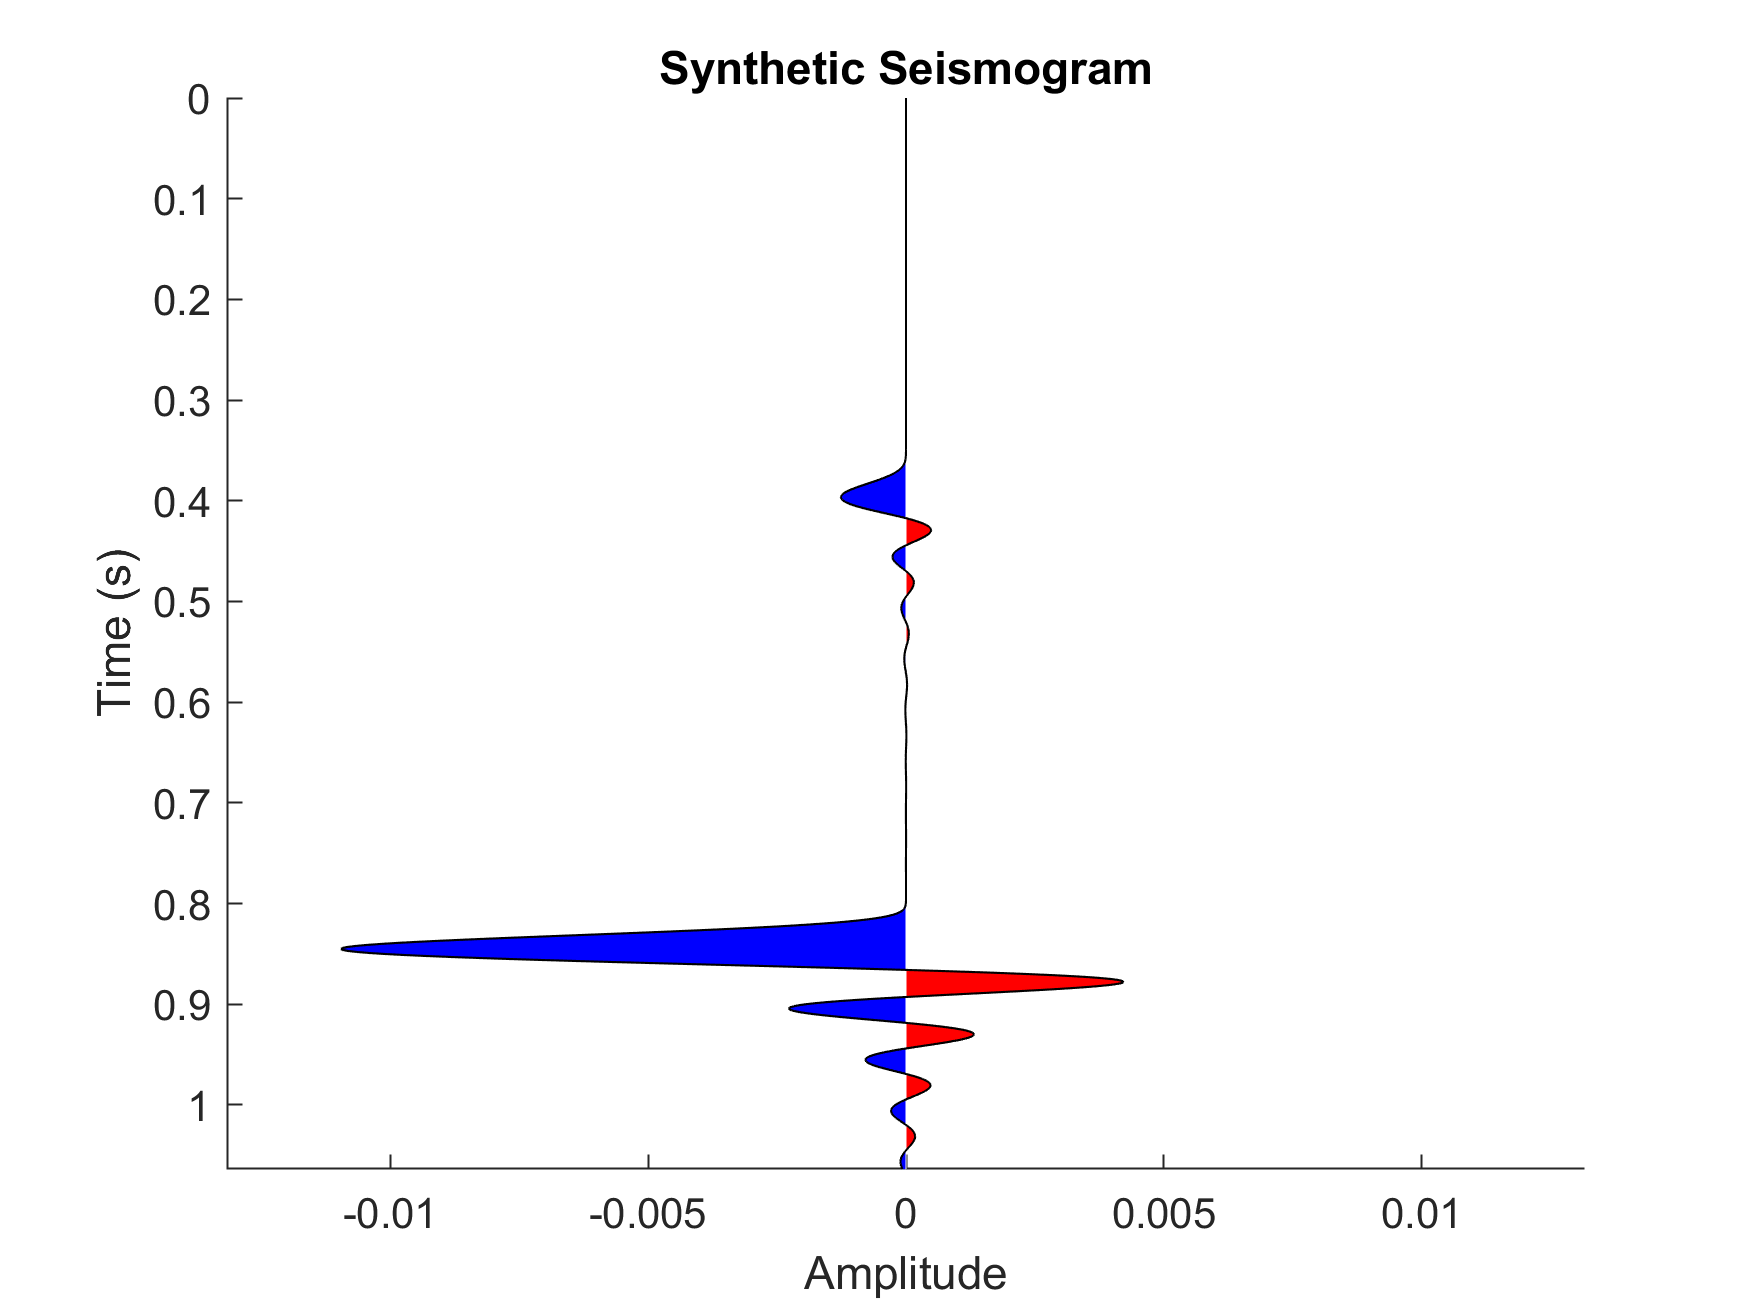
\includegraphics[width=0.8\textwidth]{Figures/RT3SyntheticSeismogram.png}
	\caption[Ray-tracing 3-layer synthetic seismogram]{Synthetic seismogram found from ray-tracing}
	\label{fig:RT3Syn}
\end{figure}

\begin{figure}[!htb]
	\centering
	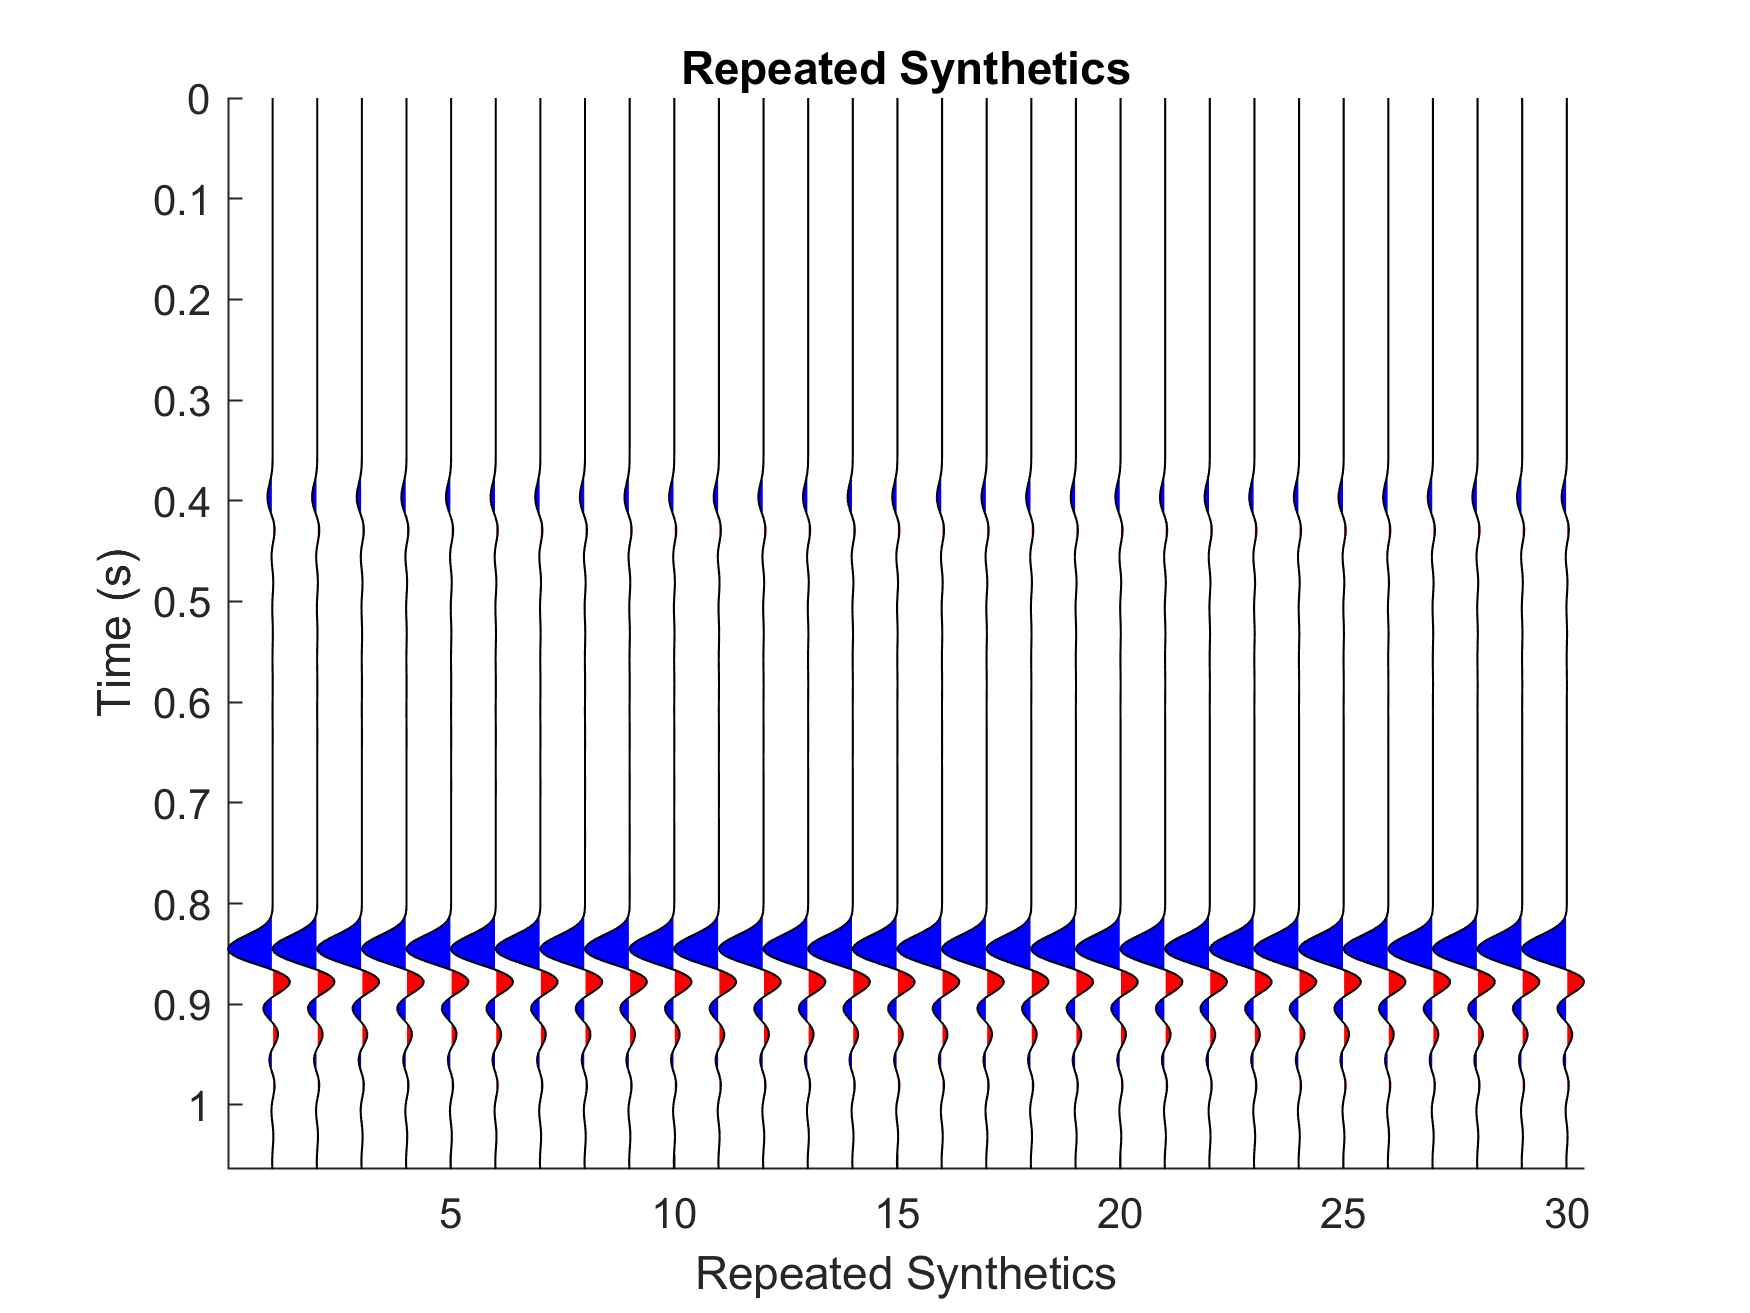
\includegraphics[width=0.8\textwidth]{Figures/RT3SeveralSynthetics.png}
	\caption[Ray-tracing 3-layer several synthetic seismograms]{Several identical synthetic seismograms found from ray-tracing}
	\label{fig:RT3Synsev}
\end{figure}

\begin{figure}[!htb]
	\centering
	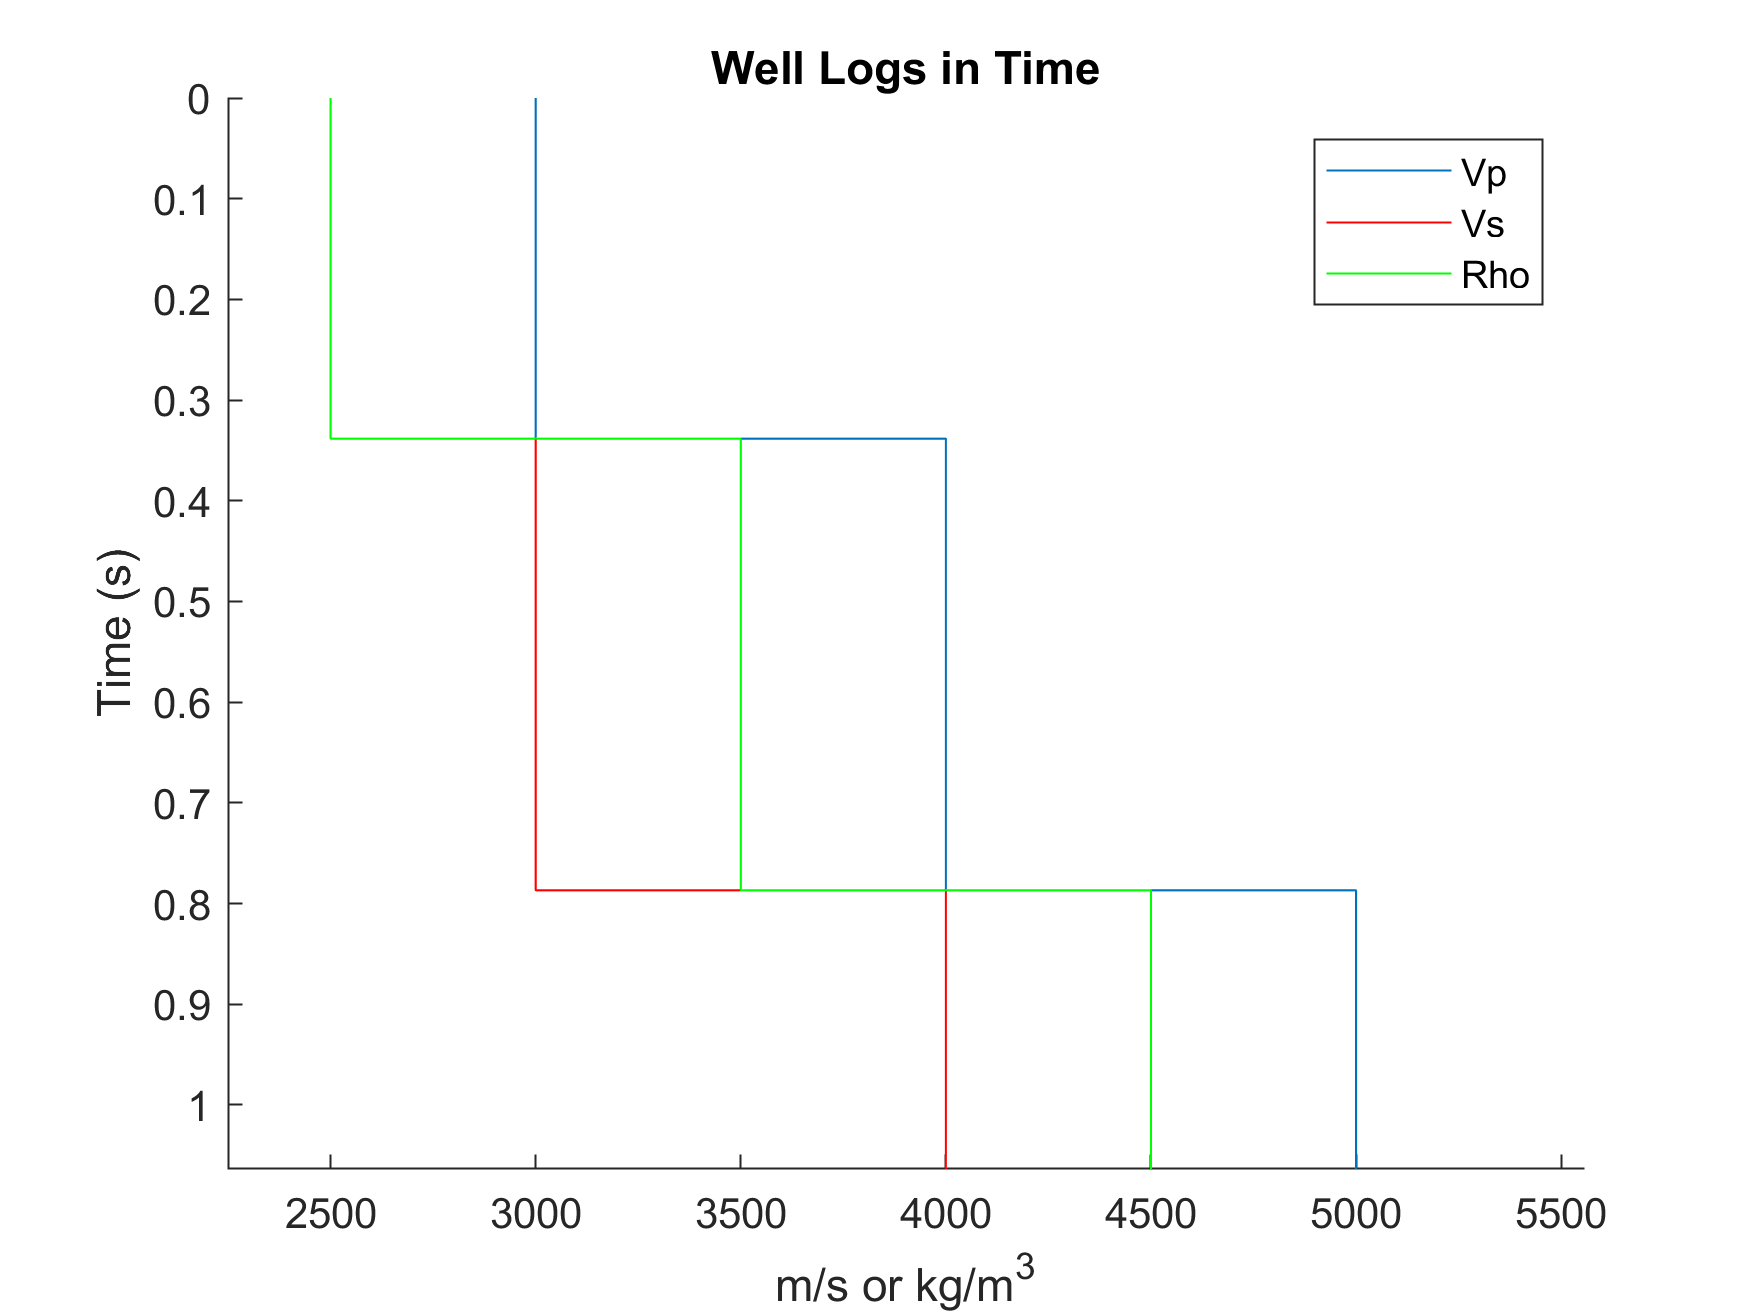
\includegraphics[width=0.8\textwidth]{Figures/RT3LogsinTime.png}
	\caption[Ray-tracing 3-layer time-converted well logs]{Well logs that have been converted into the time domain}
	\label{fig:RT3TimeLog}
\end{figure}

	Ray-tracing is a much less computationally intensive task when compared to finite-difference modelling. This simplistic approach is easier to understand and implement, however it does not model the earth as well as the previous method. Future work can be completed to account for the effects of multiples, anisotropy and other seismic effects. 
\FloatBarrier
\section{Results}
\subsection{Fox Creek Case Study}
	Hydraulic fracturing is an unconventional resource extraction method where fluids are injected into a reservoir at high pressures, fracturing the rock, allowing for oil and gas to be extracted \citep{eaton2018}. This method of extraction is becoming frequently used in regions around Fox Creek, Alberta which overlays the Duvernay formation. This formation is of the upper/late Devonian period and is composed of laminated bituminous shale, calcareous shale and dense argillaceous limestone \citep{campbell1968}. According to the Alberta Energy Regulator, the formation holds an estimated 443 trillion cubic feet of natural gas, and 61.7 billion barrels of oil \citep{Duvernay2016}.

	Because these large reserves have become recently commercially viable, oil and gas firms are setting up extraction facilities in the area. These companies are constantly trying to make their processes more efficient, safe and profitable. Because of this, there have been many academic studies in the area including work done by \cite{eaton2018} and \cite{german2018}. These studies use modern and innovative techniques to characterize the reservoir and the fracturing that occurs. 
	
	Figure \ref{fig:FCLogs} illustrates the geophysical logs for a well in the Fox Creek region (figure from \cite{german2018}) and this data will be used to test the applicability of the synthetic seismograms. In this example, there is only P-P reflection seismic data available, but both P-P and P-S seismograms will be created. The sonic log measures the P-wave velocity, the dipole sonic log measures the S-wave velocity and these will be combined with the density log to generate the synthetic. The wavelet used is identical to the previous example, as illustrated previously in figure \ref{fig:3Wavelet}. The processes shown below are for P-S reflections - P-P reflections are shown in the appendix. 

\begin{figure}[!htb]
	\centering
	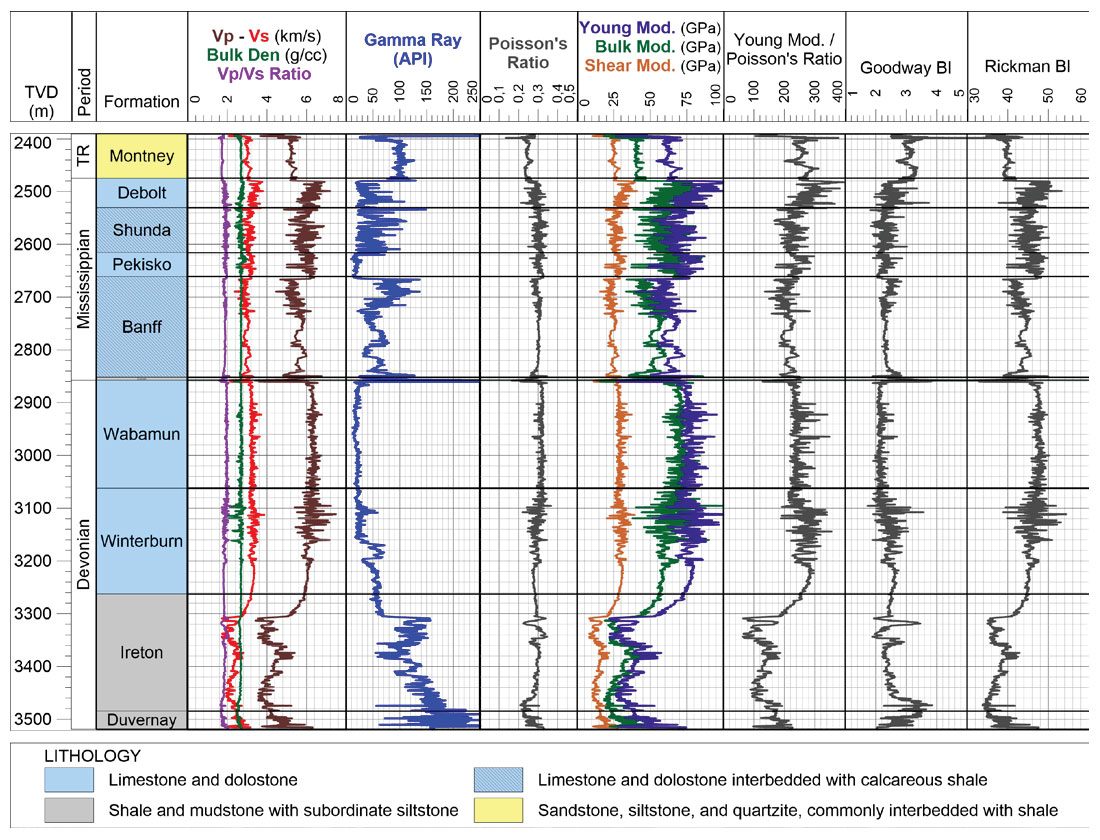
\includegraphics[width=0.9\textwidth]{Figures/duvernayLogs.jpg}
	\caption[Fox Creek well logs]{Well logs from a well in the fox creek region \citep{german2018}}
	\label{fig:FCLogs}
\end{figure}

	First, the finite-difference algorithm is used to create a synthetic. The .las well log files are converted to a usable format in MATLAB (figure \ref{fig:FCmlog} in the appendix). The log is then smoothed using a 50 point smoothing window, so the finite-difference algorithm produces cleaner results, shown in figure \ref{fig:FDClog}. 

\begin{figure}[!htb]
	\centering
	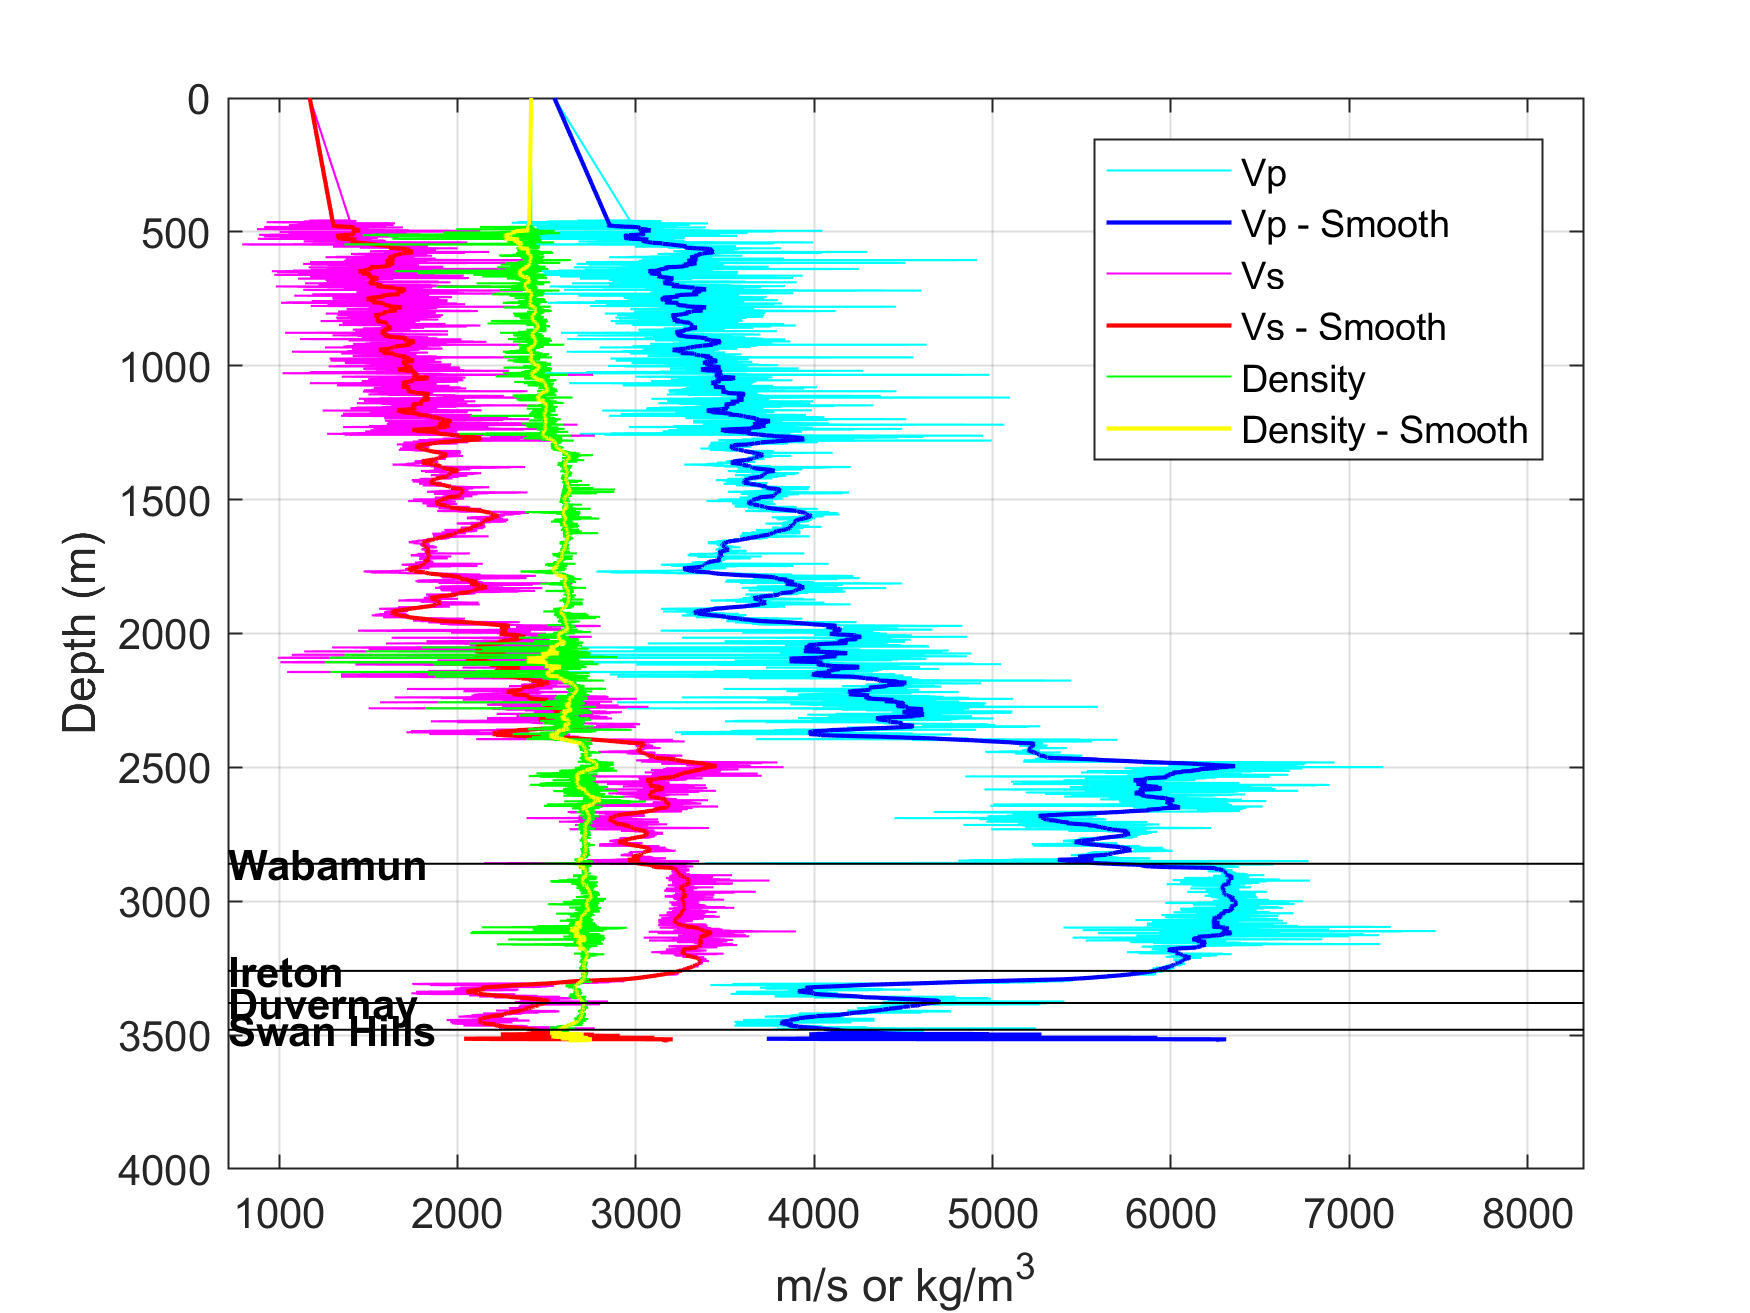
\includegraphics[width=0.8\textwidth]{Figures/FDCsmoothLog.png}
	\caption[Fox Creek finite-difference earth model]{Input well log compared with the smoothed earth model used for finite-difference modelling}
	\label{fig:FDClog}
\end{figure}

	In this case, our earth model has a grid spacing of $5m$, is $8,000m$ wide and $3,400m$ deep. The total time recorded is $2.8s$ and the sample rate is $0.0005s$ to ensure that the Courant condition is met and grid dispersion is minimized. On a dual-core CPU with a clock speed of $2.7 GHz$, the model and processing corrections took approximately 3 hours to complete.  The full uncorrected P-S output gather is seen in figure \ref{fig:FDCXgather}.

\begin{figure}[!htb]
	\centering
	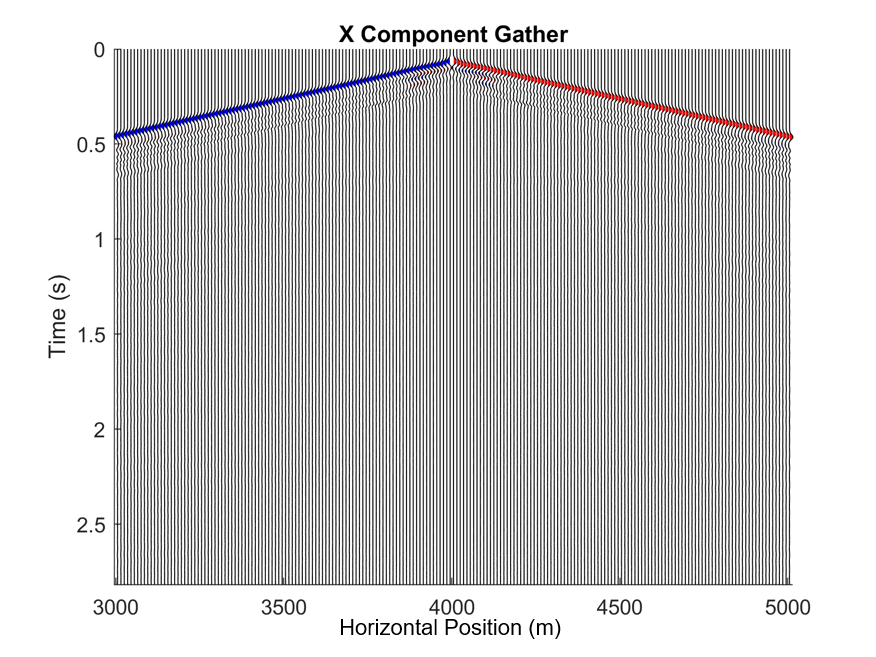
\includegraphics[width=0.7\textwidth]{Figures/FDCXgather.png}
	\caption[Fox Creek finite-difference P-S gather]{Uncorrected P-S output gather from the finite-difference tool}
	\label{fig:FDCXgather}
\end{figure}	
	
	The gain correction is applied by using an AGC window of $0.5s$ and the velocities are corrected using NMO (figures \ref{fig:FDCgain} and \ref{fig:FDCnmo} respectively, in the appendix). The traces are then summed and averaged to create a stacked trace, or in this case, the synthetic seismogram shown in figure \ref{fig:FDCstack}.
	
\begin{figure}[!htb]
	\centering
	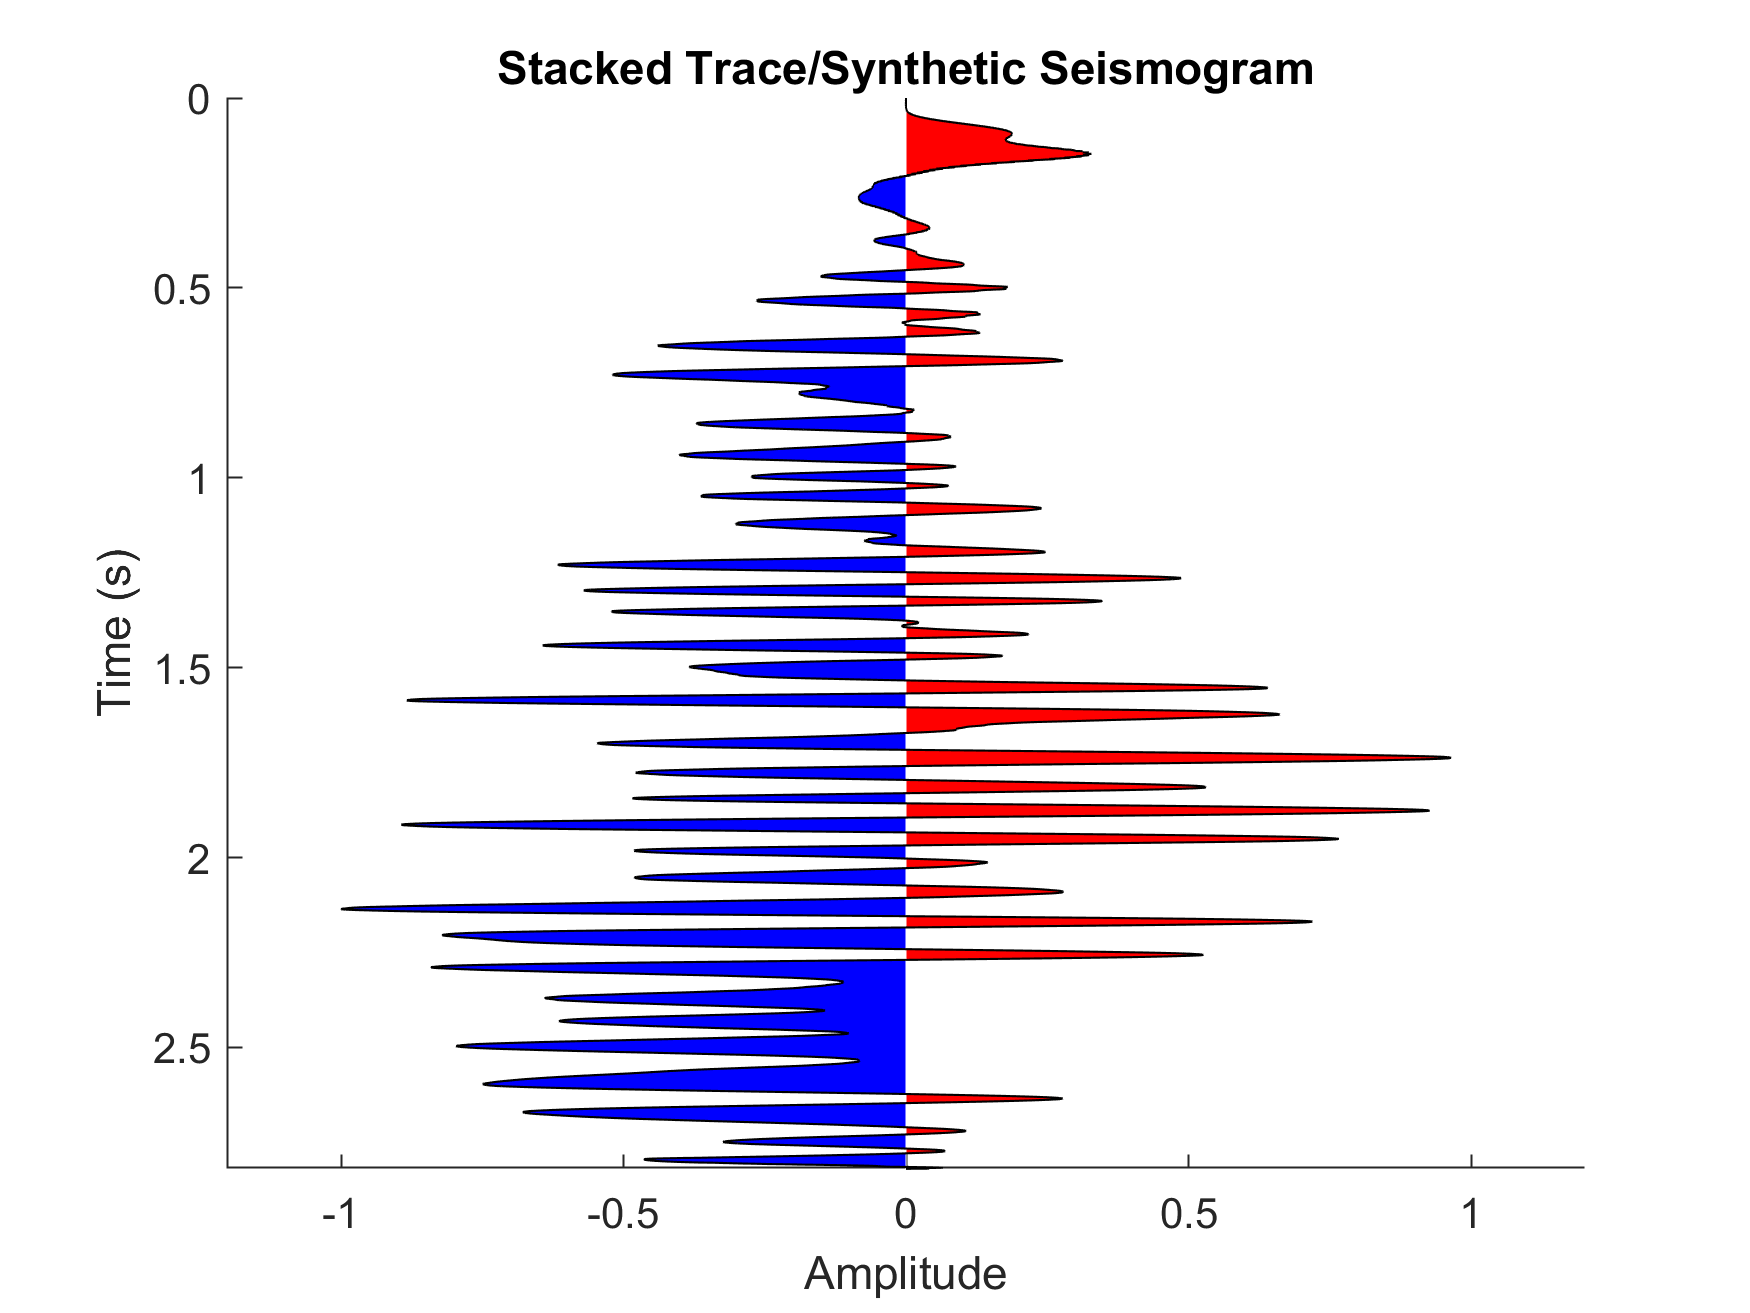
\includegraphics[width=0.7\textwidth]{Figures/FDCstack.png}
	\caption[Fox Creek finite-difference P-S synthetic seismogram]{Stacked trace and the synthetic seismogram from finite-difference P-S modelling}
	\label{fig:FDCstack}
\end{figure}	
	
	Next, the ray-tracing algorithm will be used to create a synthetic. Using the same input logs (figure \ref{fig:FCLogs}) as the finite-difference method, the model is divided into 100 layers of constant thickness and the logs are averaged for each layer, as shown in figure \ref{fig:RTCLogs}. 

\begin{figure}[!htb]
	\centering
	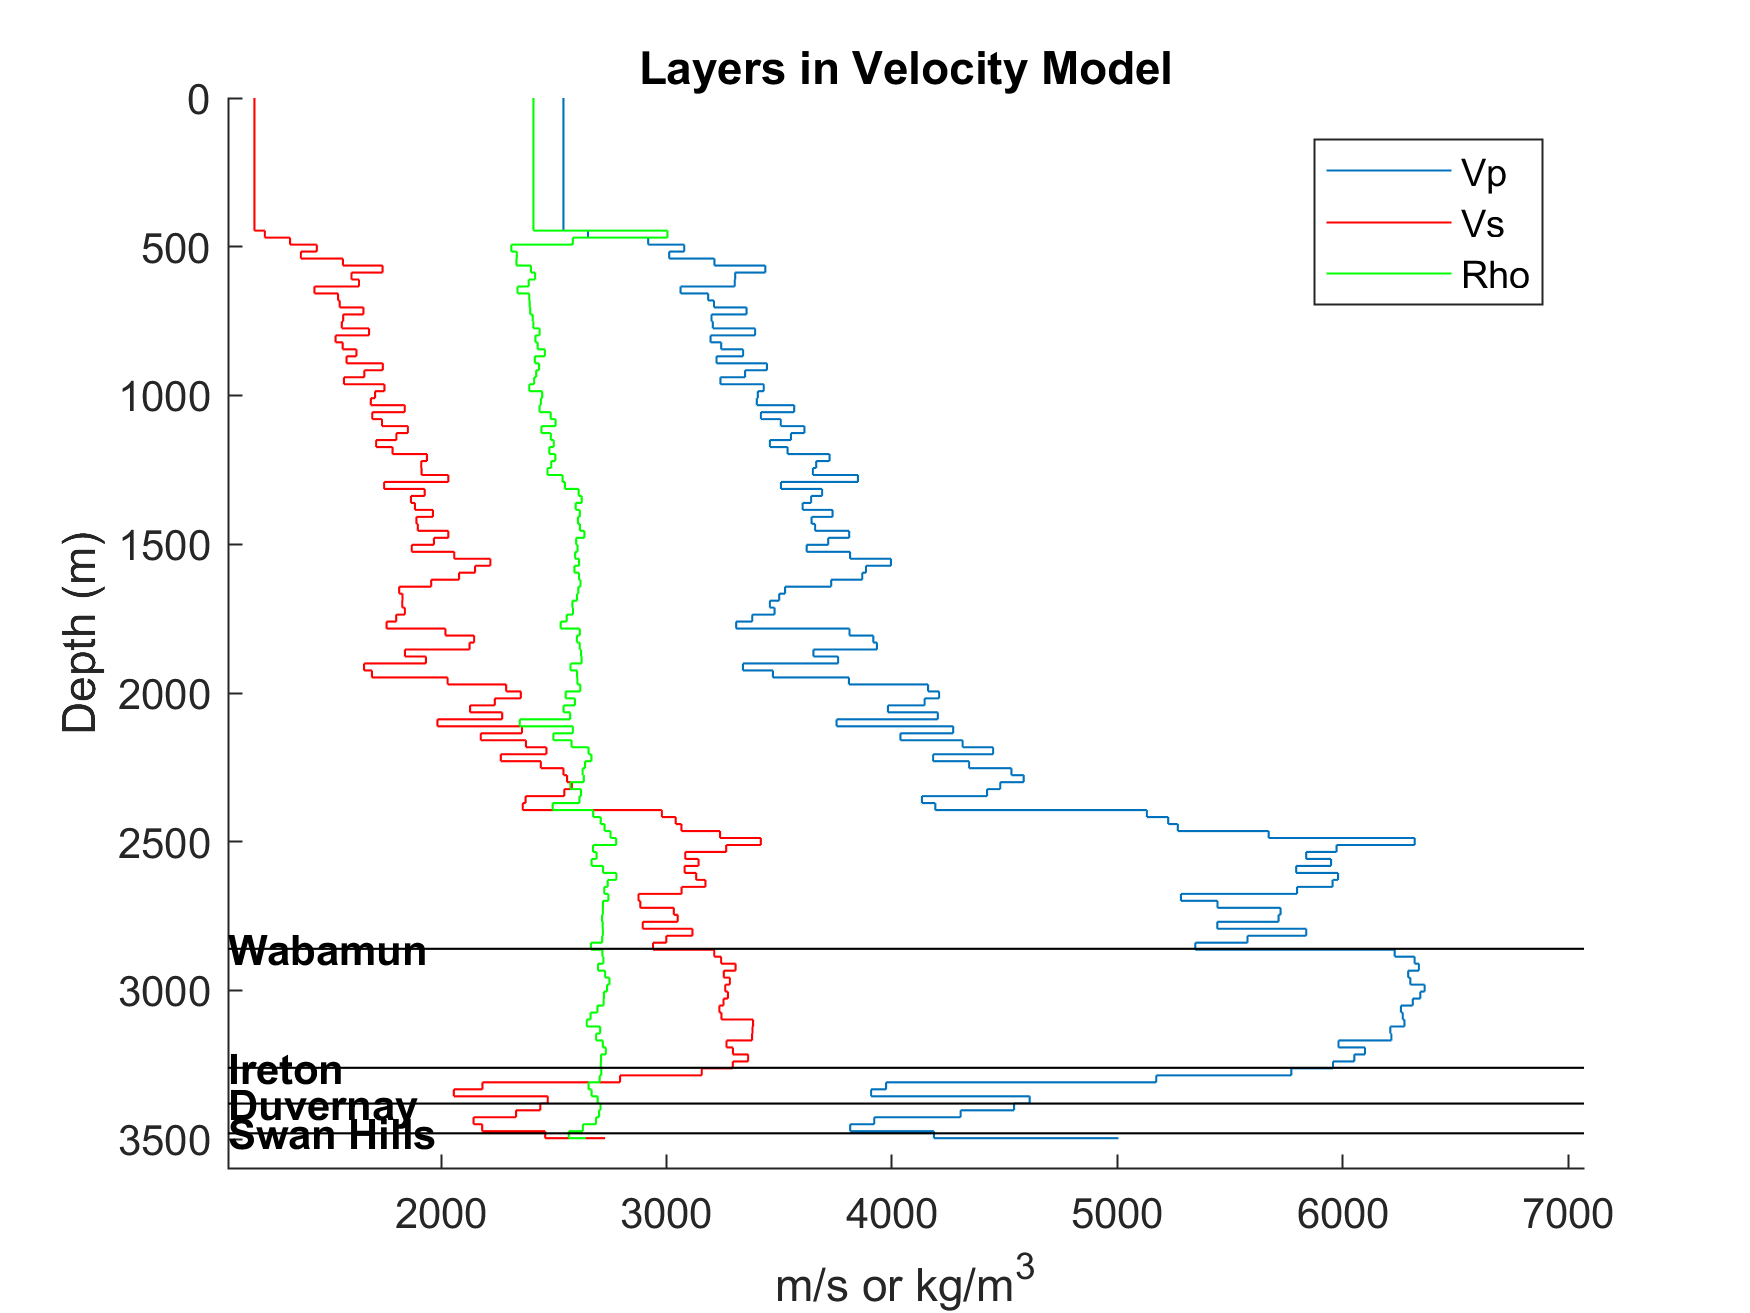
\includegraphics[width=0.7\textwidth]{Figures/RTCLayers.png}
	\caption[Fox Creek ray-tracing layered model]{Earth model divided into layers of constant thickness for ray-tracing}
	\label{fig:RTCLogs}
\end{figure}

	There is the question of the optimal amount of layers needed before there stops being noticeable changes. There are a lot of factors that determine this answer including wavelet type and frequency, target depth, input ray angle increment and the seismic data itself that you are trying to analyze. There is not a simple formula to answer this question but seeing as the ray-tracing method does not take much computing time, having a large number of layers (100-200) is recommended. However, if there are too many layers and the frequency of the wavelet is not low enough, the synthetic can be too high-frequency to properly match the seismic. In this case, 150 layers were sufficient. 
	
\FloatBarrier

	Next, a fan of rays is sent through the earth by varying the input angle by 1 degree and the results are interpolated to match an offset of $1000m$ (approximately the average offset in a nearby seismic survey), shown in figure \ref{fig:RTCinterp}. Notice how the P-S reflection points become asymptotic as depth increases.  There is also a question of what ray increment should be used and I found that a 1-degree interval works very well in almost all cases as this tends to interpolate all deep layers very well, with a maximum error in this case of $30m$ away from the specified offset. This error occurs at the most shallow reflection point and as depth increases, the error decreases and all of the offsets become very close to the specified offset very quickly. If the goal is to image shallow layers at high-offsets, the degree interval should be decreased. Alternatively, if there are many layers in the earth model, the degree interval should also be lowered. With these parameters, the algorithm took approximately 30 seconds to complete. 

\begin{figure}[!htb]
	\centering
	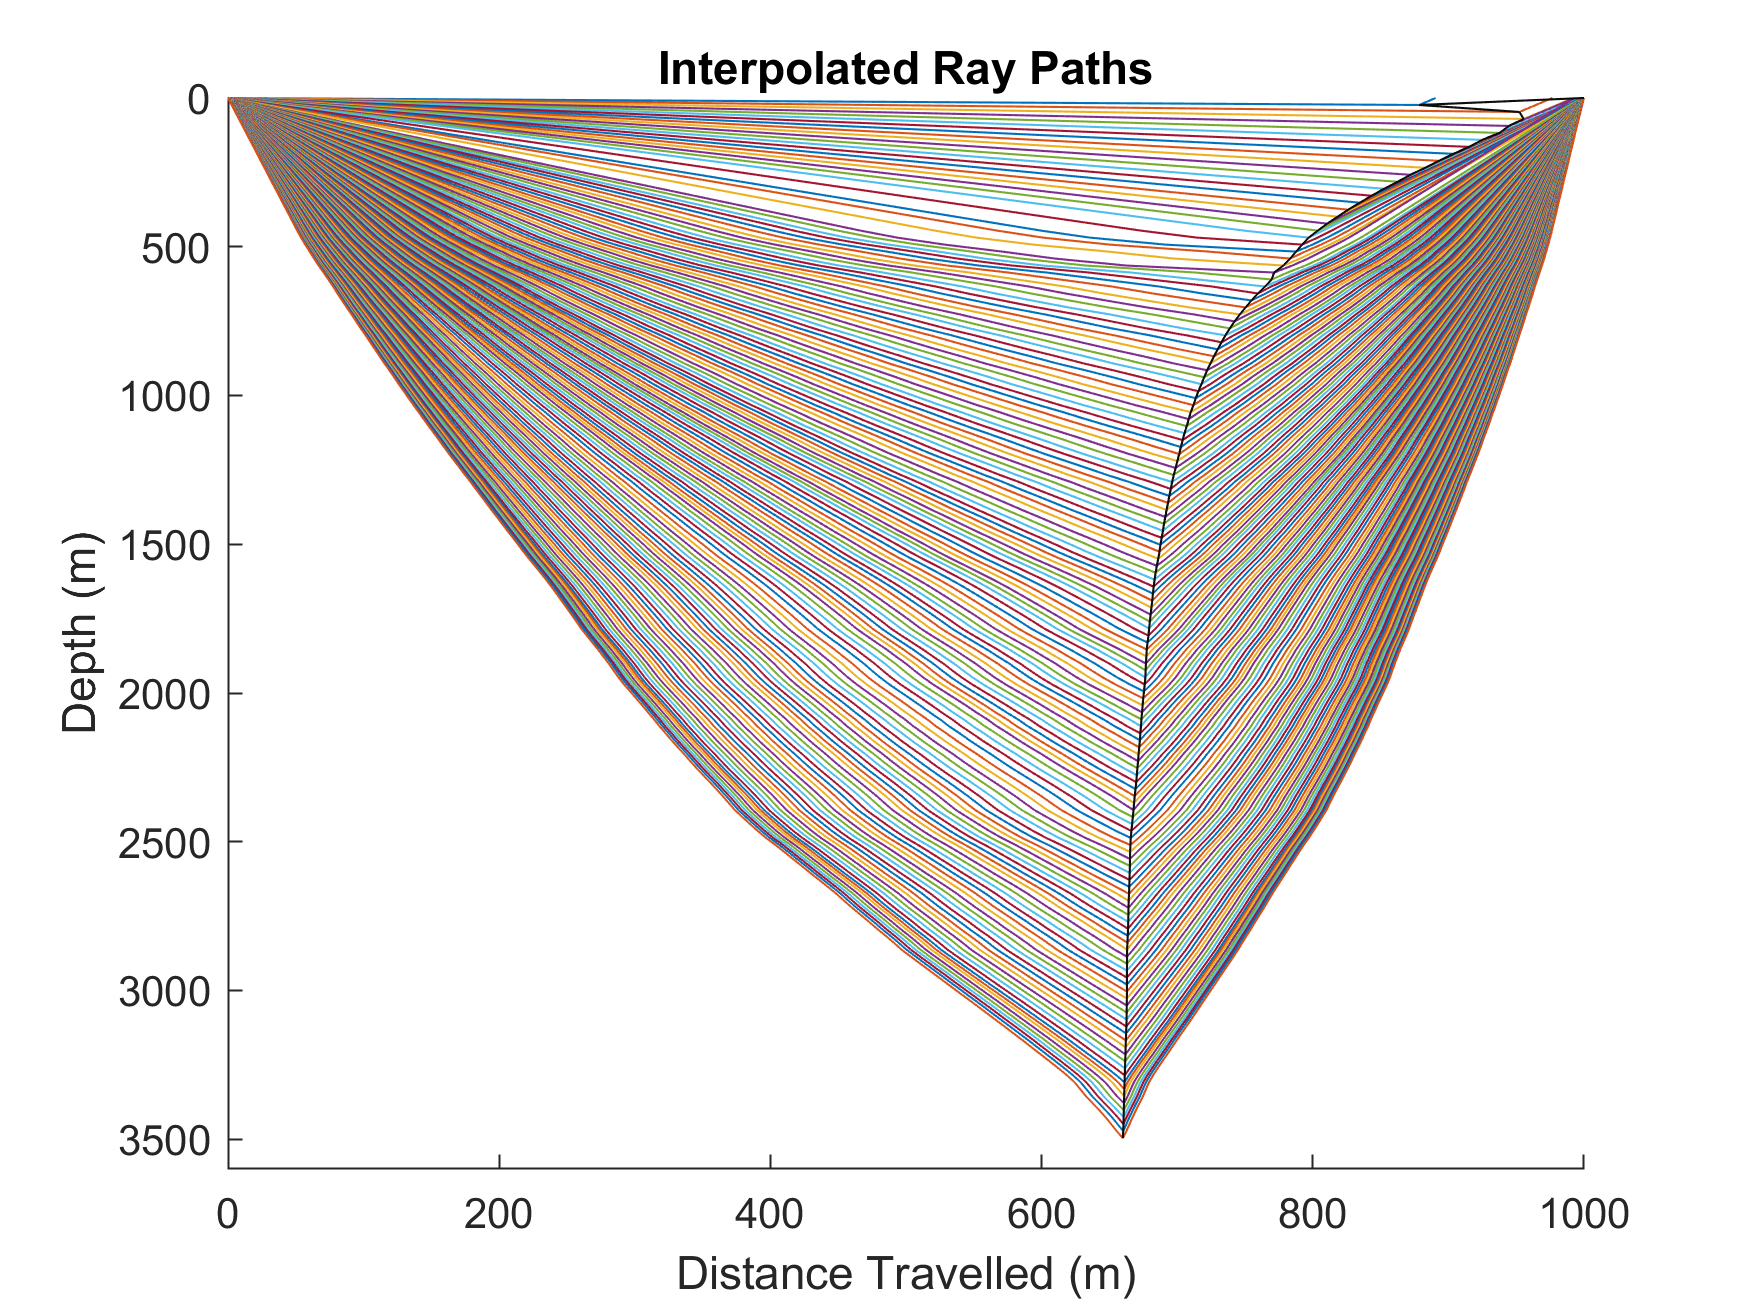
\includegraphics[width=0.8\textwidth]{Figures/RTCinterp.png}
	\caption[Fox Creek ray-tracing ray-paths]{Interpolated P-S ray-paths }
	\label{fig:RTCinterp}
\end{figure}

	The amplitudes at each reflection point are calculated using the Zoeppritz equations and are matched with the zero-offset travel times, creating a reflectivity series (figure \ref{fig:RTCrefseries}). This is then convolved with a wavelet (figure \ref{fig:3Wavelet}, above) to create a synthetic seismogram, shown in figure \ref{fig:RTCsynthetic}. We will compare the P-P finite-difference and ray-tracing versions of the synthetics with seismic and compare these two methods with each other, in the next section.

\begin{figure}[!htb]
	\centering
	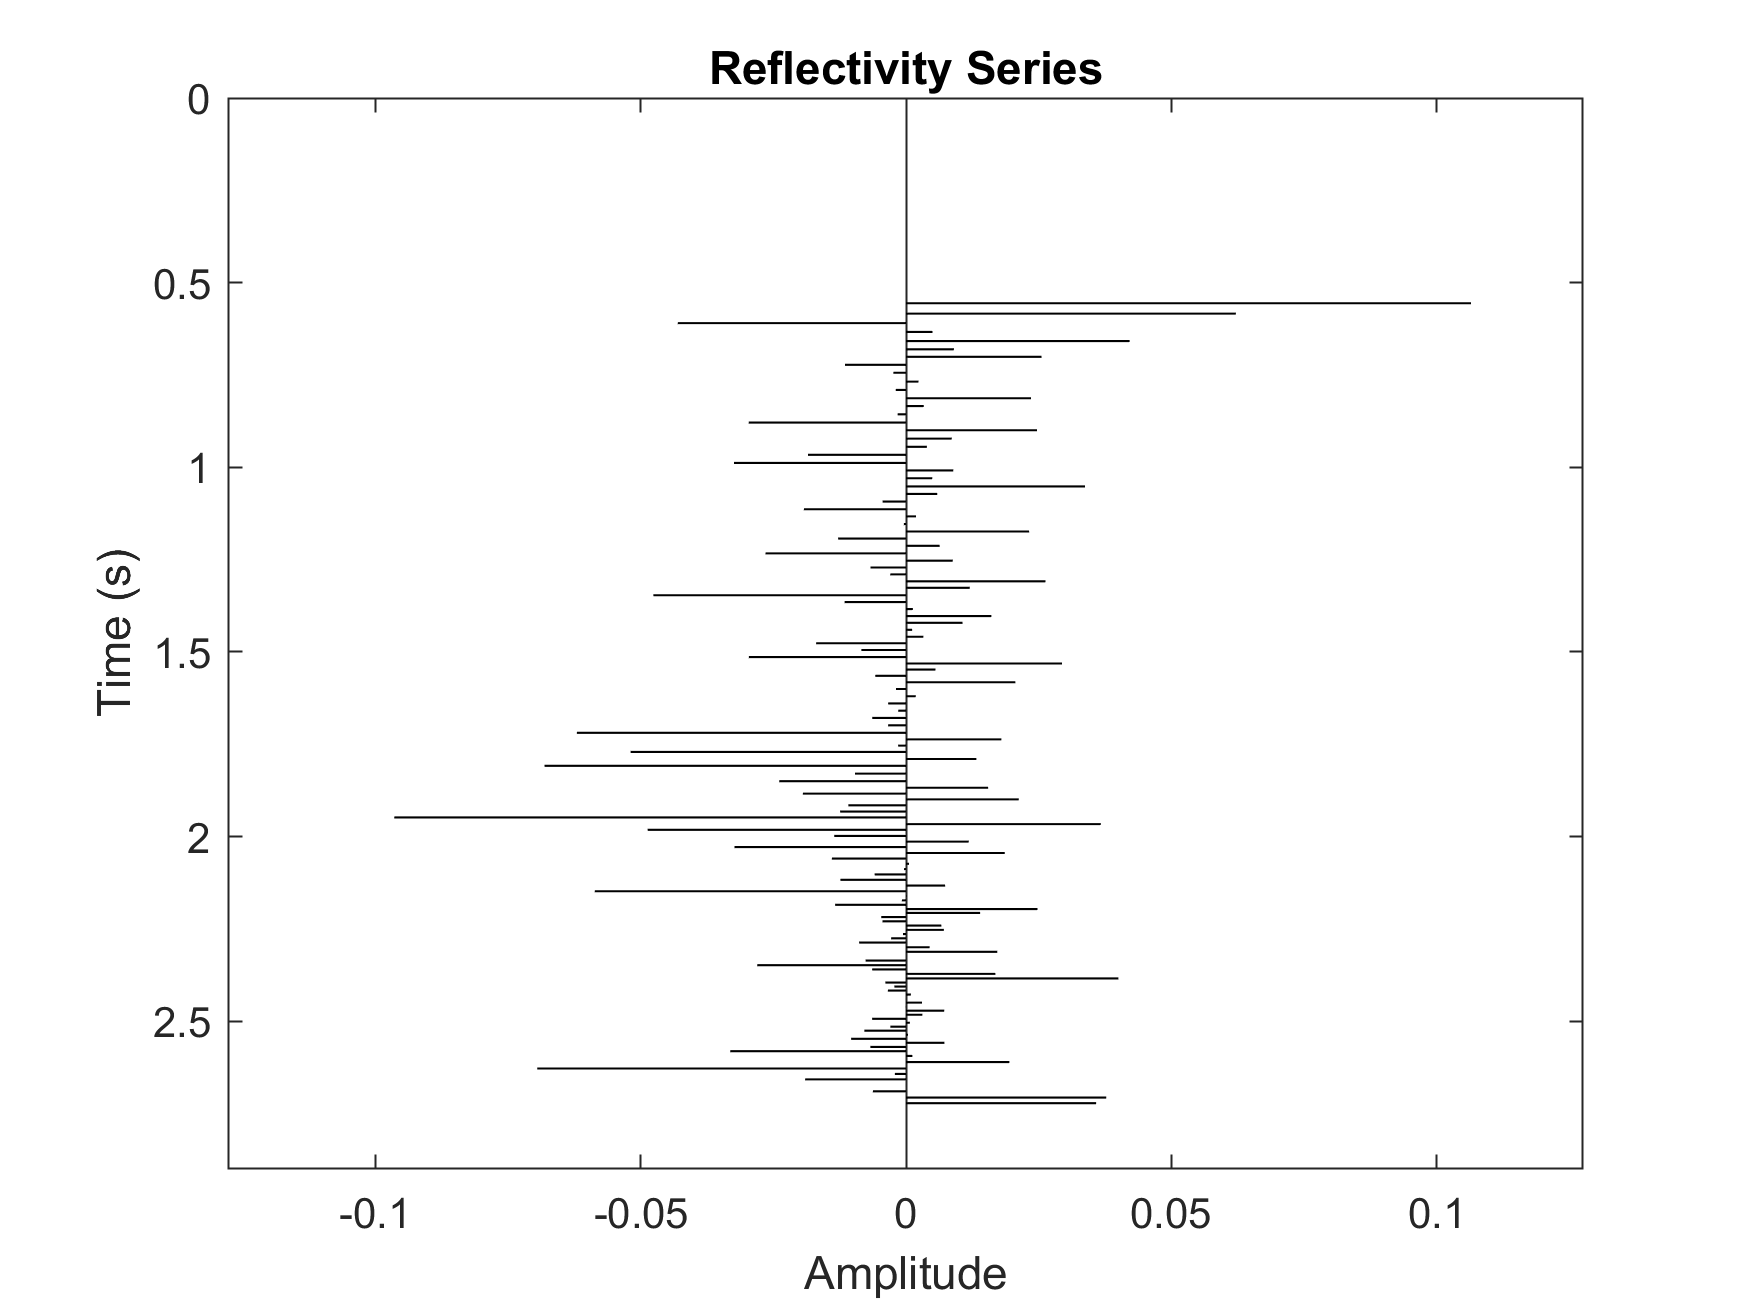
\includegraphics[width=0.8\textwidth]{Figures/RTCrefseries.png}
	\caption[Fox Creek ray-tracing P-S reflectivity series]{Reflectivity Series for P-S reflections from ray-tracing}
	\label{fig:RTCrefseries}
\end{figure}	

\begin{figure}[!htb]
	\centering
	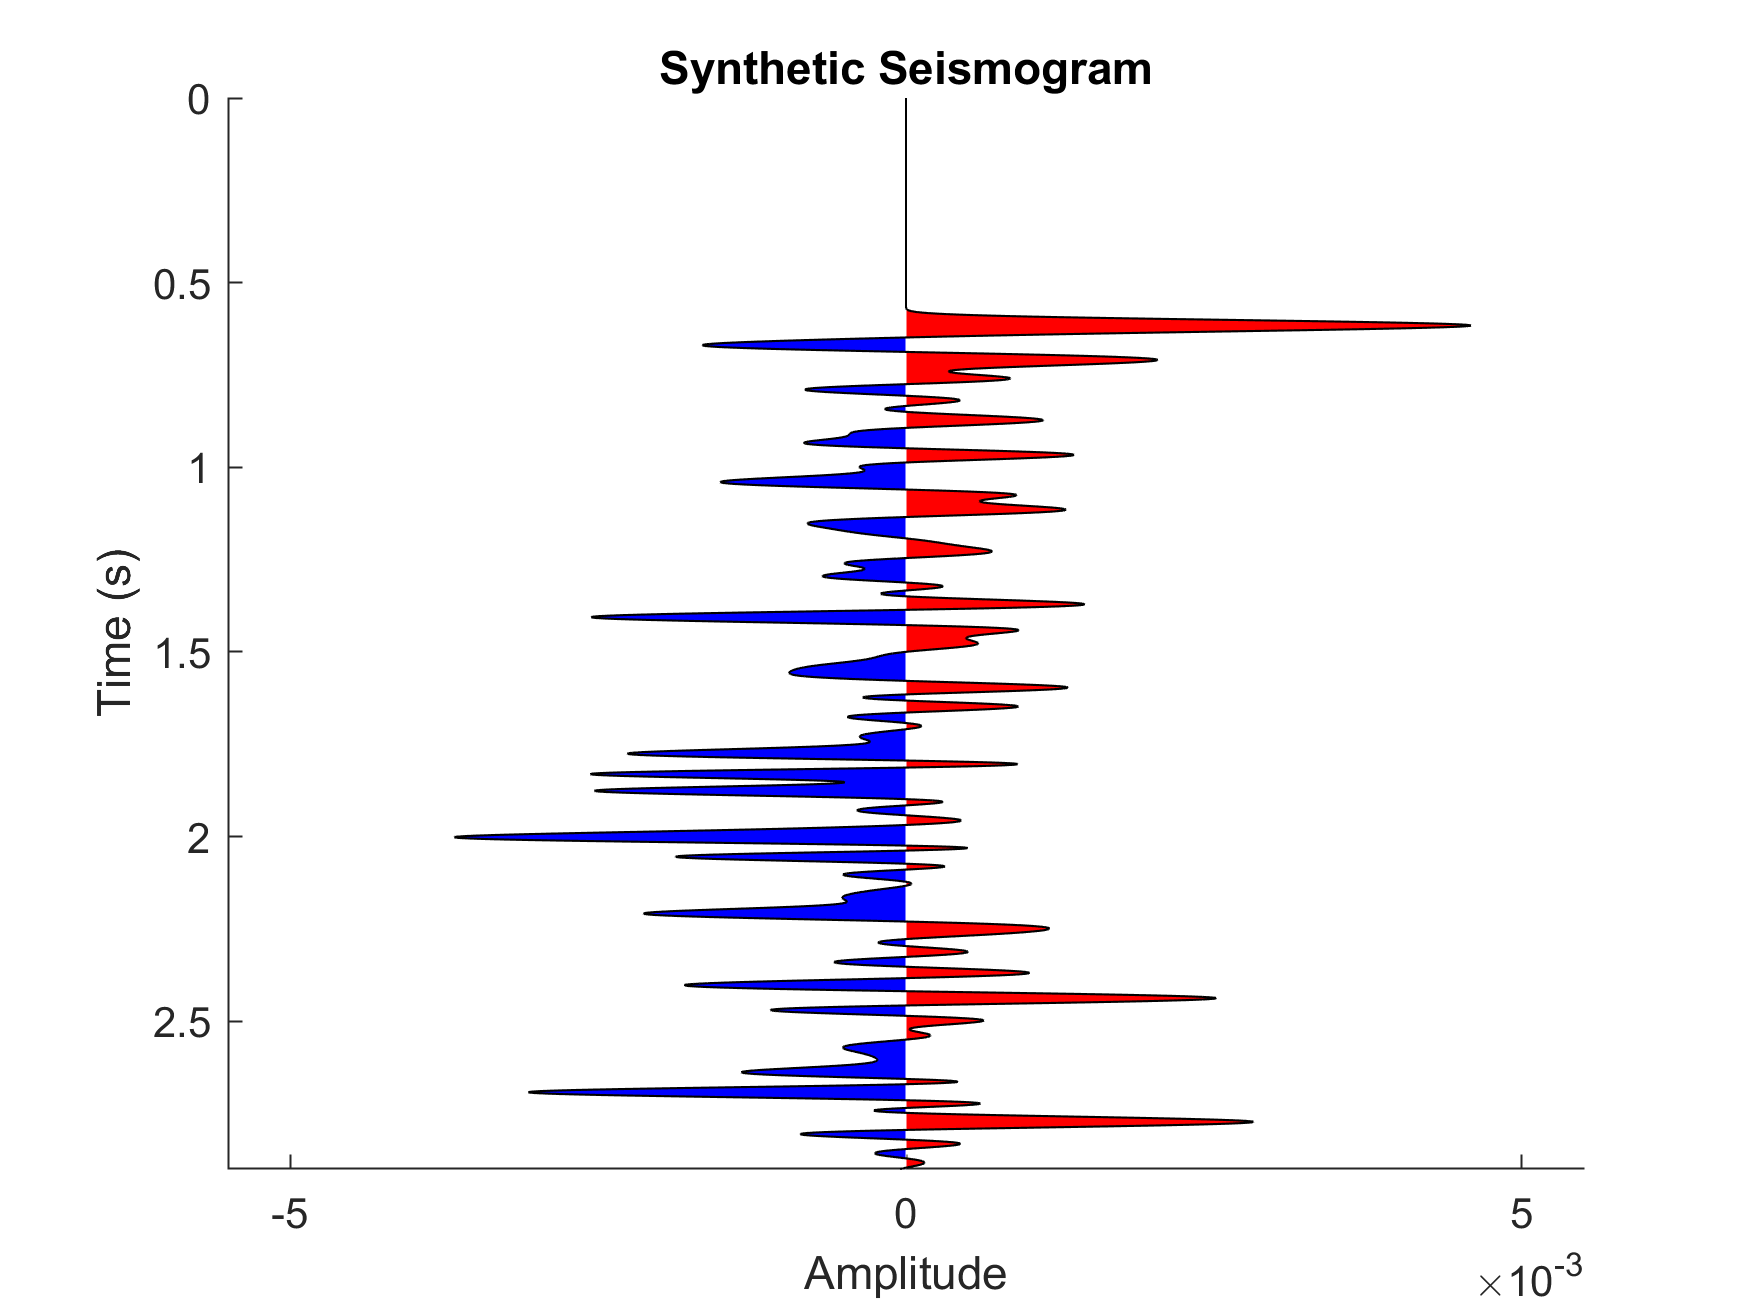
\includegraphics[width=0.8\textwidth]{Figures/RTCsynthetic.png}
	\caption[Fox Creek ray-tracing P-S synthetic seismogram]{Synthetic seismogram for P-S reflections from ray-tracing}
	\label{fig:RTCsynthetic}
\end{figure}	

\begin{figure}[!htb]
	\centering
	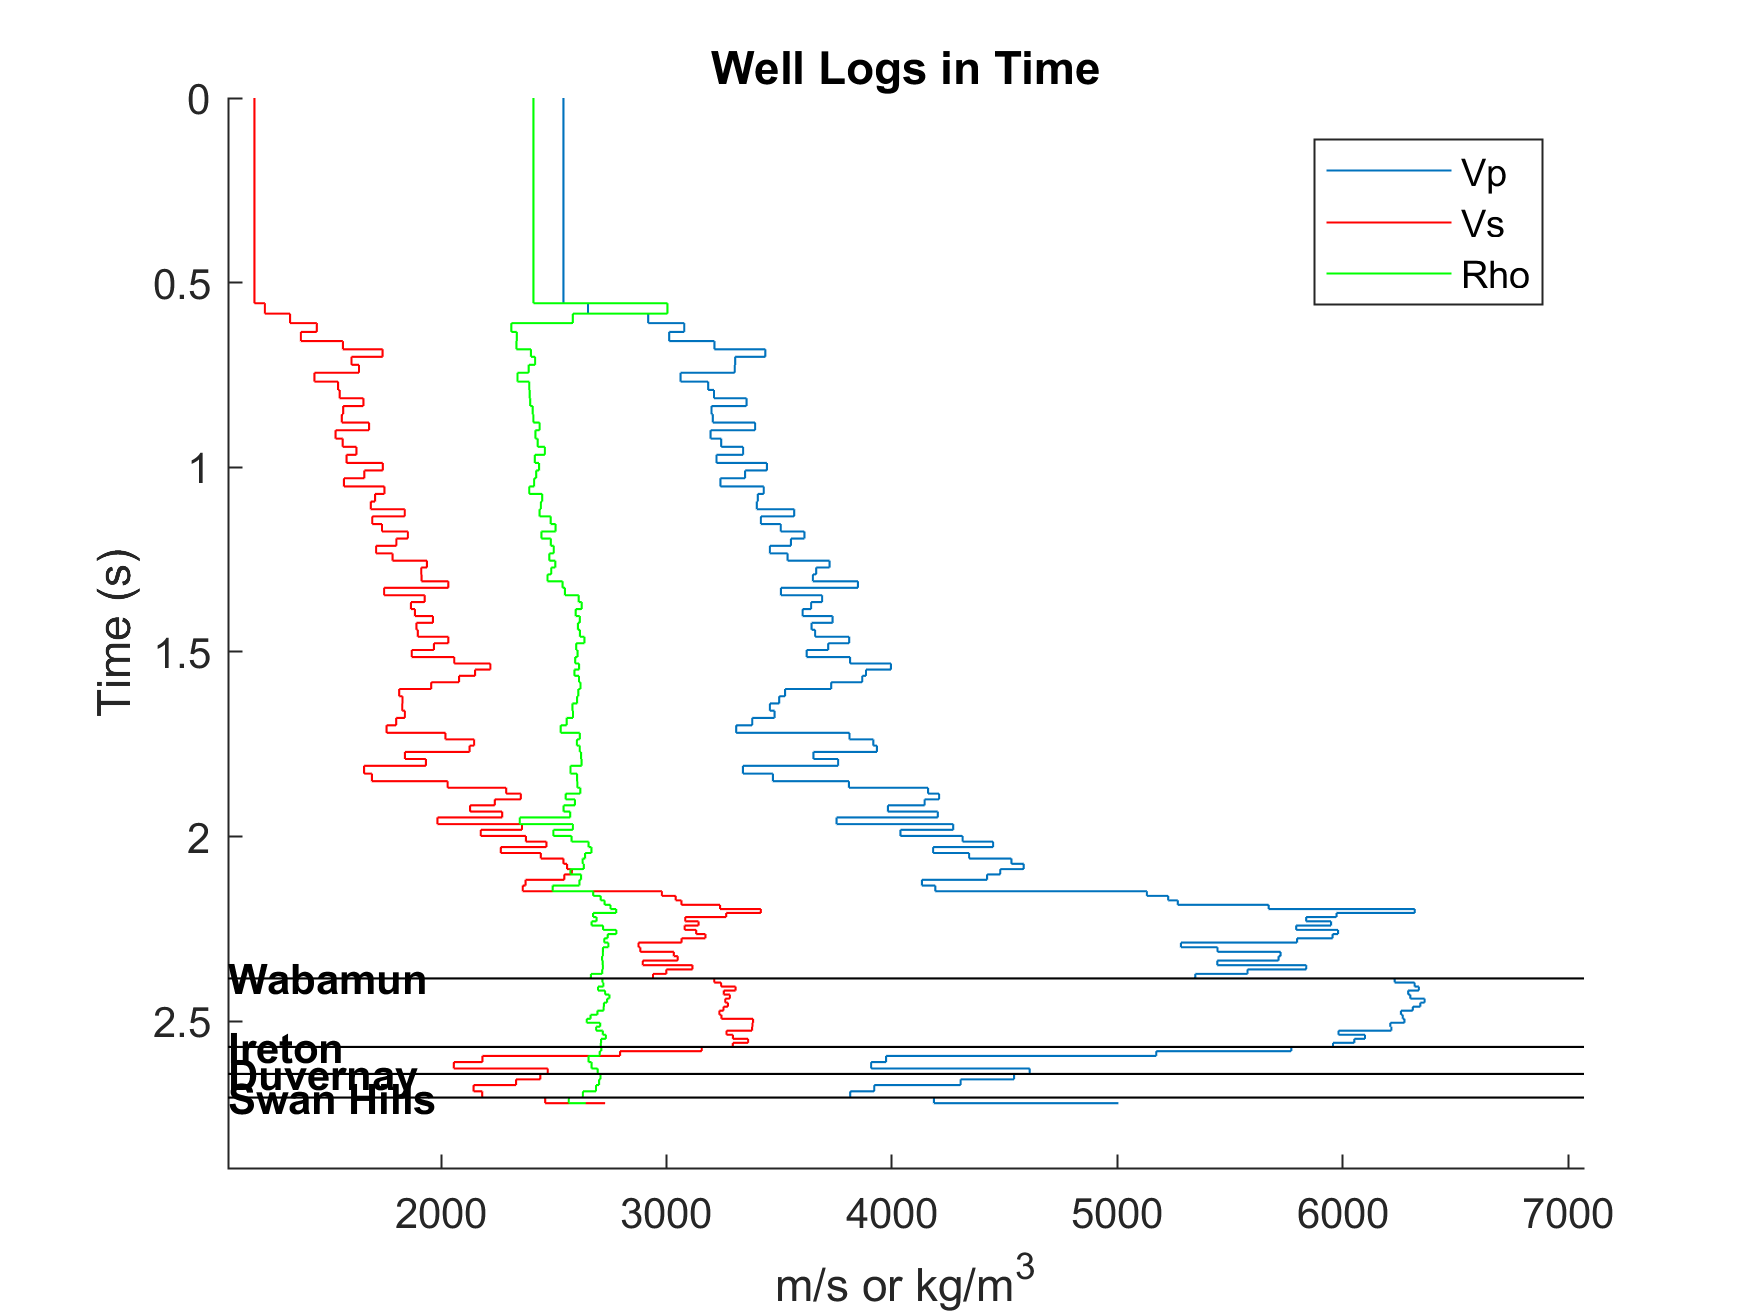
\includegraphics[width=0.8\textwidth]{Figures/RTCtimelogs.png}
	\caption[Fox Creek ray-tracing P-S well logs in time]{Well logs converted from depth to time using the time-depth-relationship from P-S reflections}
	\label{fig:RTCtimelogs}
\end{figure}
\FloatBarrier	

\subsection{Comparisons}

	The seismic used to compare with the synthetics is a pre-stack time-migrated (PSTM) East-West capture of a 3D volume in the Fox Creek region, taken from \cite{german2018} (figure \ref{fig:FCseis}). The seismic displays horizon interpretations for the Wabamun, Ireton, Duvernay, Swan Hills and Precambrian basement. The red lines in this figure display a projection of horizontal wells and the green dots indicate seismic and microseismic events in the area. These are not applicable in this study. Only a P-P seismic section was available and because of this, P-P versions of the finite-difference and ray-tracing techniques will be used in the comparison.
	
\begin{figure}[!htb]
	\centering
	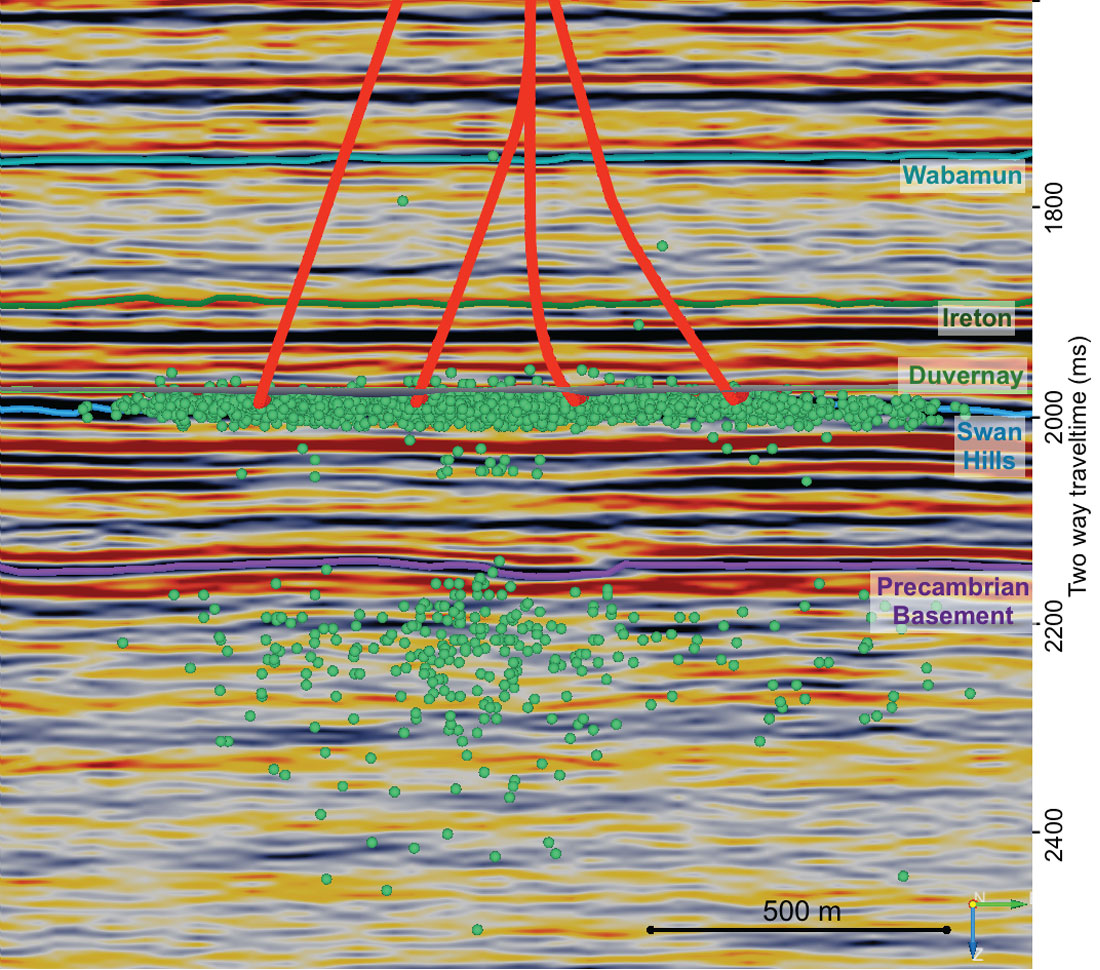
\includegraphics[width=0.6\textwidth]{Figures/FCseis.jpg}
	\caption[Fox Creek interpreted seismic section]{This seismic section will be used to make comparisons with the synthetic seismograms.The red lines are a cross-section of horizontal wells and the green dots are microseismic and seismic events.  Seismic section from \cite{german2018}. }
	\label{fig:FCseis}
\end{figure}
	
	The well was drilled in a region outside of the seismic cube, but given the horizontal nature of the Wabamun, Ireton, Duvernay and Swan Hills formation interpretations, it can be appropriate to lay the synthetic beside the seismic intersection. 30 identical synthetic seismograms are displayed beside each other and the window is enlarged in the area of interest to aid in interpretations. On a final note before the comparisons, well tops were only converted from depth to time using the ray-tracing method, as the process for creating a time-depth-relationship using finite-difference methods is a difficult task and not necessary for the scope of this comparison.
	
	Figure \ref{fig:FDseis} shows a direct comparison between the finite-difference generated synthetic and a seismic section in the area. The well tops in the figure have been taken from their ray-tracing counterpart. Despite attempting several different gain windows, all of the amplitudes in this section appear similar in magnitude which makes the synthetic very difficult to interpret. The amplitudes between the Wabamum and Ireton interpretations should be fairly low, as indicated by the seismic, but on the seismogram, this is not the case. This could also be a velocity artifact that came into effect when the traces were stacked without having a perfect velocity correction. On the seismic, the Wabamun is interpreted on a large trough but on the synthetic, it is right between two troughs. The Ireton seismic peak matches with a synthetic S-crossing (zero amplitude between a trough and a peak), the Duvernay peak matches with an S-crossing on the synthetic as well and the large Swan Hills trough matches with a very small trough on the synthetic. These errors in correlation could be from a phase difference between the seismic and the synthetic, or they could be from choosing the wrong input wavelet. Regardless of where the errors came from, a lot of time was spent to get these to match as closely as possible with little results. This shows that the finite-difference method can be very difficult to properly calibrate to match with the seismic.	
	
\begin{figure}[!htb]
	\centering
	\includegraphics[width=0.9\textwidth]{Figures/FDseis.jpg}
	\caption[Fox Creek seismic finite-difference comparison]{Comparison between a finite-difference generated synthetic and a seismic section in the same region. Note that the well tops on the synthetic are generated from taking the respective interval time location from the ray-tracing method. Seismic section from \cite{german2018}. }
	\label{fig:FDseis}
\end{figure}	
	
	Next, figure \ref{fig:RTseis} shows a comparison between the ray-tracing generated synthetic and a seismic section in the area. Again, the seismic shows that the region between the Wabamun and Ireton interpretations should be fairly low energy and this is exactly what the synthetic shows. The Wabamun seismic trough matches with an S-crossing on the seismic, the Ireton seismic peak matches with an area of low amplitude on the synthetic, the Duvernay peak matches with a small peak on the synthetic and the Swan Hills trough matches with a trough on the synthetic. As above, these errors can be corrected by choosing a different input wavelet or by phase shifting the seismic to match. There is a large trough on the synthetic above the Wabamun, which could match with the large trough on the synthetic, however there are no horizon interpretations available for this reflector to make this correlation.

\begin{figure}[!htb]
	\centering
	\includegraphics[width=0.9\textwidth]{Figures/RTseis.jpg}
	\caption[Fox Creek seismic ray-tracing comparison]{Comparison between a ray-tracing generated synthetic and a seismic section in the same region. Seismic section from \cite{german2018}. }
	\label{fig:RTseis}
\end{figure}	

	Synthetics are not typically generated with the wavelet used in this example. This wavelet was chosen as it can be applied to both the finite-difference and ray-tracing methods easily, allowing for a direct comparison between them. Figure \ref{fig:RTseisr} shows a comparison between the seismic and a $20 Hz$, zero-phase Ricker wavelet, which is much more commonly used for synthetic generation. Images for this synthetic alone are available in the appendix. Here we can see that the Wabamun seismic trough matches with a trough on the synthetic, the Ireton seismic peak matches with a synthetic peak, the Duvernay peak matches with an S-crossing, as does the Swan Hills trough. These correlations have been improved with the change in wavelet and can be improved even more with a higher frequency wavelet and more accurate well top picks. 

\begin{figure}[!htb]
	\centering
	\includegraphics[width=0.9\textwidth]{Figures/RTseisr.jpg}
	\caption[Fox Creek seismic ray-tracing comparison (Ricker wavelet)]{Comparison between a ray-tracing generated synthetic and a seismic section in the same region. The wavelet is a $20 Hz$, zero-phase Ricker wavelet. Seismic section from \cite{german2018}.}
	\label{fig:RTseisr}
\end{figure}

	Both the ray-tracing and finite-difference time signatures do not match up perfectly with the seismic data. This shows that there still needs to be a velocity correction applied to the seismograms in both cases, which is typical of synthetic generations. The synthetics will have to be stretched, squeezed and bulk shifted to make an accurate time-depth-relationship for the well.
	
	When comparing the finite-difference and ray-tracing algorithms, the ray-tracing method is superior. The amplitudes better match the seismic data, the well logs and interpretations can be easily converted from depth to time and the synthetic generation computing time is lower by several orders of magnitude. The finite-difference method does model the subsurface much more accurately, however, it accounts for several seismic effects that are typically removed or minimized during processing, such as multiples and the direct wave arrival. The signal should also be deconvolved from the wavelet as best as possible to match the seismic. There is also numerical noise and truncation errors that are involved when trying to represent a continuous operator with discrete terms. 

\section{Conclusion}

	A synthetic seismogram is a tool that is used on a very frequent basis by interpretation geophysicists throughout their careers . Having the ability to relate data in the depth domain to data in the time domain, and vice versa, is essential to provide useful information for everyone working on a team. Because the amplitude of P-Sv reflections approaches zero at zero-offset, it is crucial to have a reliable and accurate way to generate a synthetic seismogram for P-S reflection data. 
	
	Finite-difference methods approximate the wave equation to model how acoustic waves propagate through a medium. This method creates a synthetic gather which is then gain corrected, velocity corrected and stacked - creating a synthetic seismogram. The model is divided into grids and propagates at a specified time interval and these values have to be low enough to ensure that the model is stable and that grid dispersion is minimized. Setting these values at appropriate conditions results in a model that is incredibly computationally expensive and takes a very long time for a computer to run, deterring many users from using this process. The processing corrections then add another layer of complexity and possible errors to the system. Even still, this method suffers from numerical noise and truncation errors that create a signal that does not appear to match the seismic well. The benefits to this method, however, can potentially outweigh the costs as finite-difference methods can model the effects of direct waves, primary reflected waves, multiple reflected waves, surface waves, head waves, converted waves, diffracted waves and critically refracted waves. 
	
	Ray-tracing methods use Snell's Law to model how a wave will propagate through the subsurface. A fan of rays was sent into a horizontally layered earth model and then interpolated to reach a specified offset. At each reflection point, the Zoeppritz equations were used to calculate amplitudes, and these were projected back onto a zero-offset trace and convolved with a wavelet to create a synthetic seismogram. This method took far less computing time than its finite-difference counterpart and appeared to be less error-prone. This method is limited, however, in the wave types and seismic effects that it can model. Trial and error must be used to choose the layer thickness and degree increment input conditions to best match the seismic while minimizing computing time. Future work can be done to program the effects of anisotropy, account for multiples and to add a stretch and squeeze velocity correction to this method. Overall, it was demonstrated that ray-tracing methods were superior to those of finite-difference for the generation of synthetic seismograms. 


\pagebreak
\bibliographystyle{dcu}
\bibliography{509References}
\pagebreak

\section{Appendix}
\renewcommand\thefigure{A.\arabic{figure}}  
\setcounter{figure}{0}
\subsection{Fox Creek General Figures}
\begin{figure}[!htb]
	\centering
	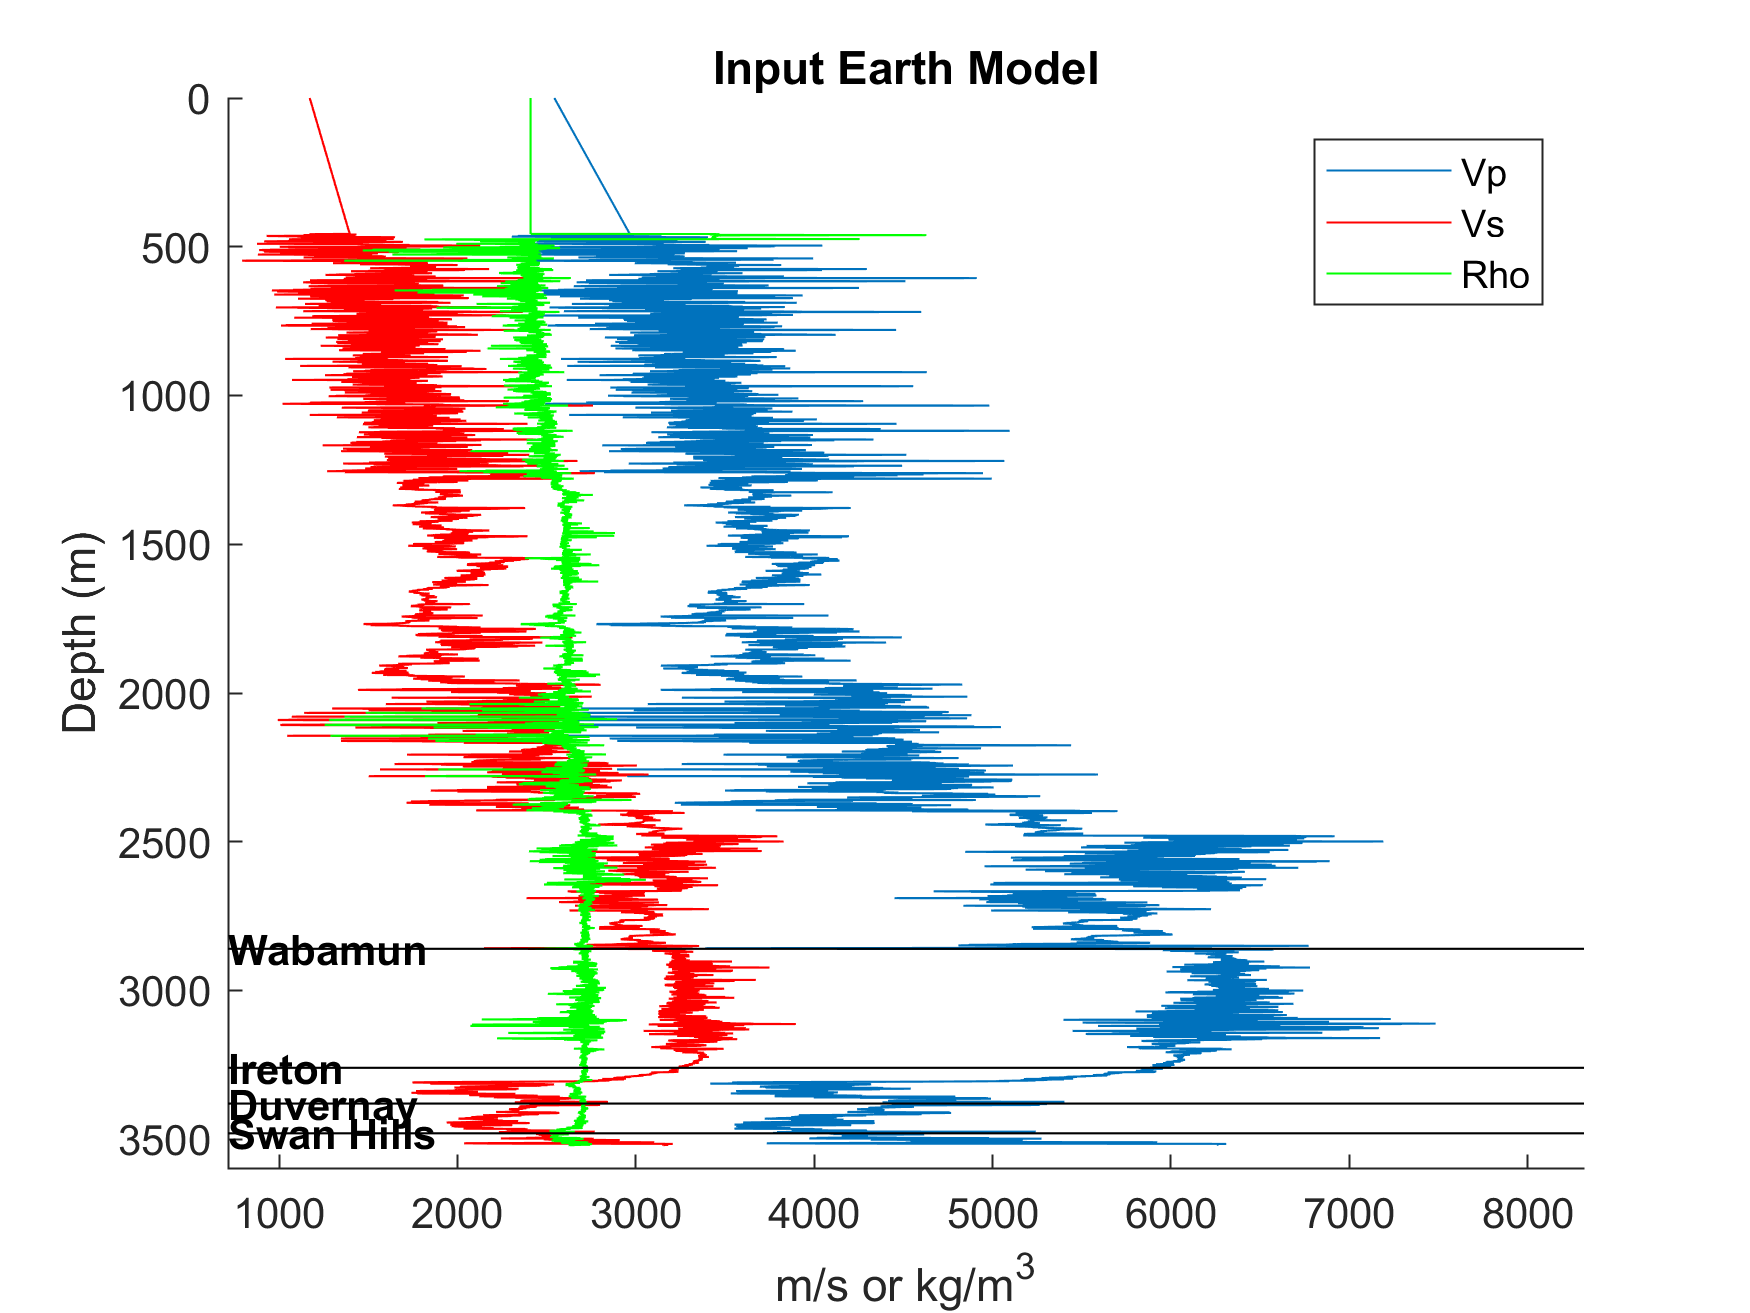
\includegraphics[width=0.8\textwidth]{Figures/FInputModel.png}
	\caption[Fox Creek MATLAB well logs]{Fox Creek well logs that are in a usable MATLAB format}
	\label{fig:FCmlog}
\end{figure}	
\FloatBarrier
\pagebreak

\subsection{Fox Creek Finite-Difference P-S}

\begin{figure}[!htb]
	\centering
	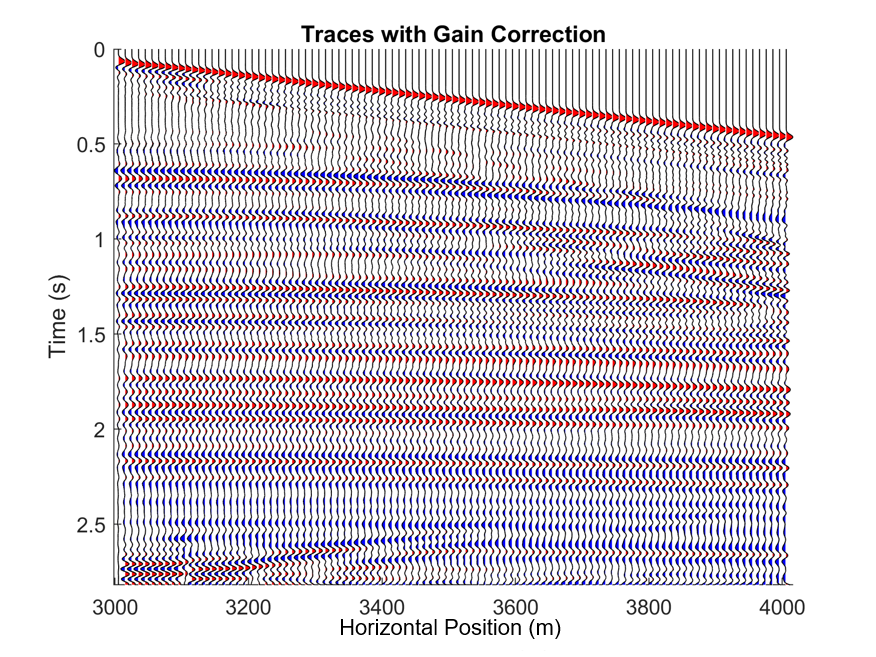
\includegraphics[width=0.7\textwidth]{Figures/FDCgain.png}
	\caption[Fox Creek finite-difference P-S gain correction]{Gain corrected Fox Creek data from finite-difference P-S modelling}
	\label{fig:FDCgain}
\end{figure}	

\begin{figure}[!htb]
	\centering
	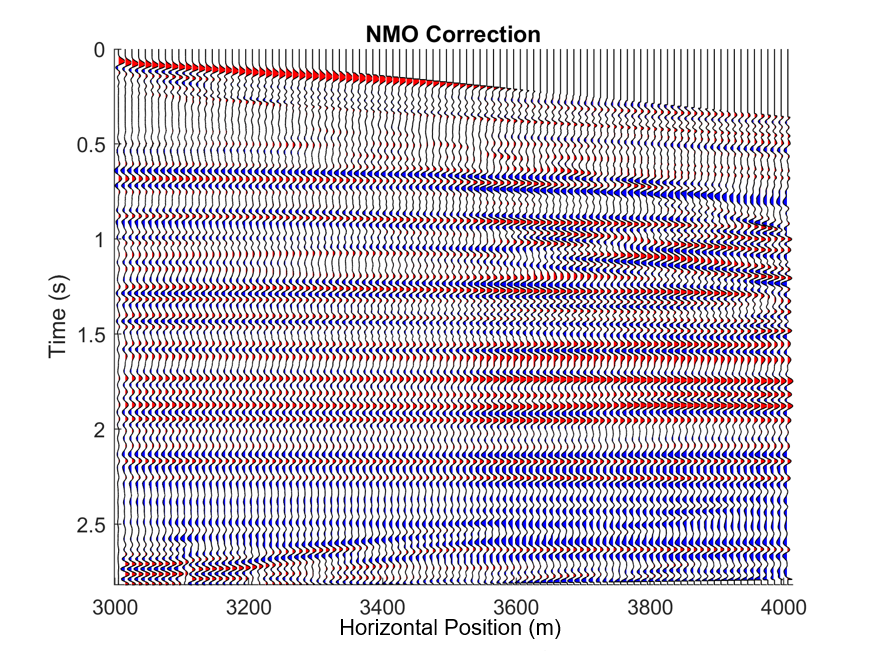
\includegraphics[width=0.7\textwidth]{Figures/FDCnmo.png}
	\caption[Fox Creek finite-difference P-S NMO correction]{Velocity corrected Fox Creek data from finite-difference P-S modelling}
	\label{fig:FDCnmo}
\end{figure}	

\begin{figure}[!htb]
	\centering
	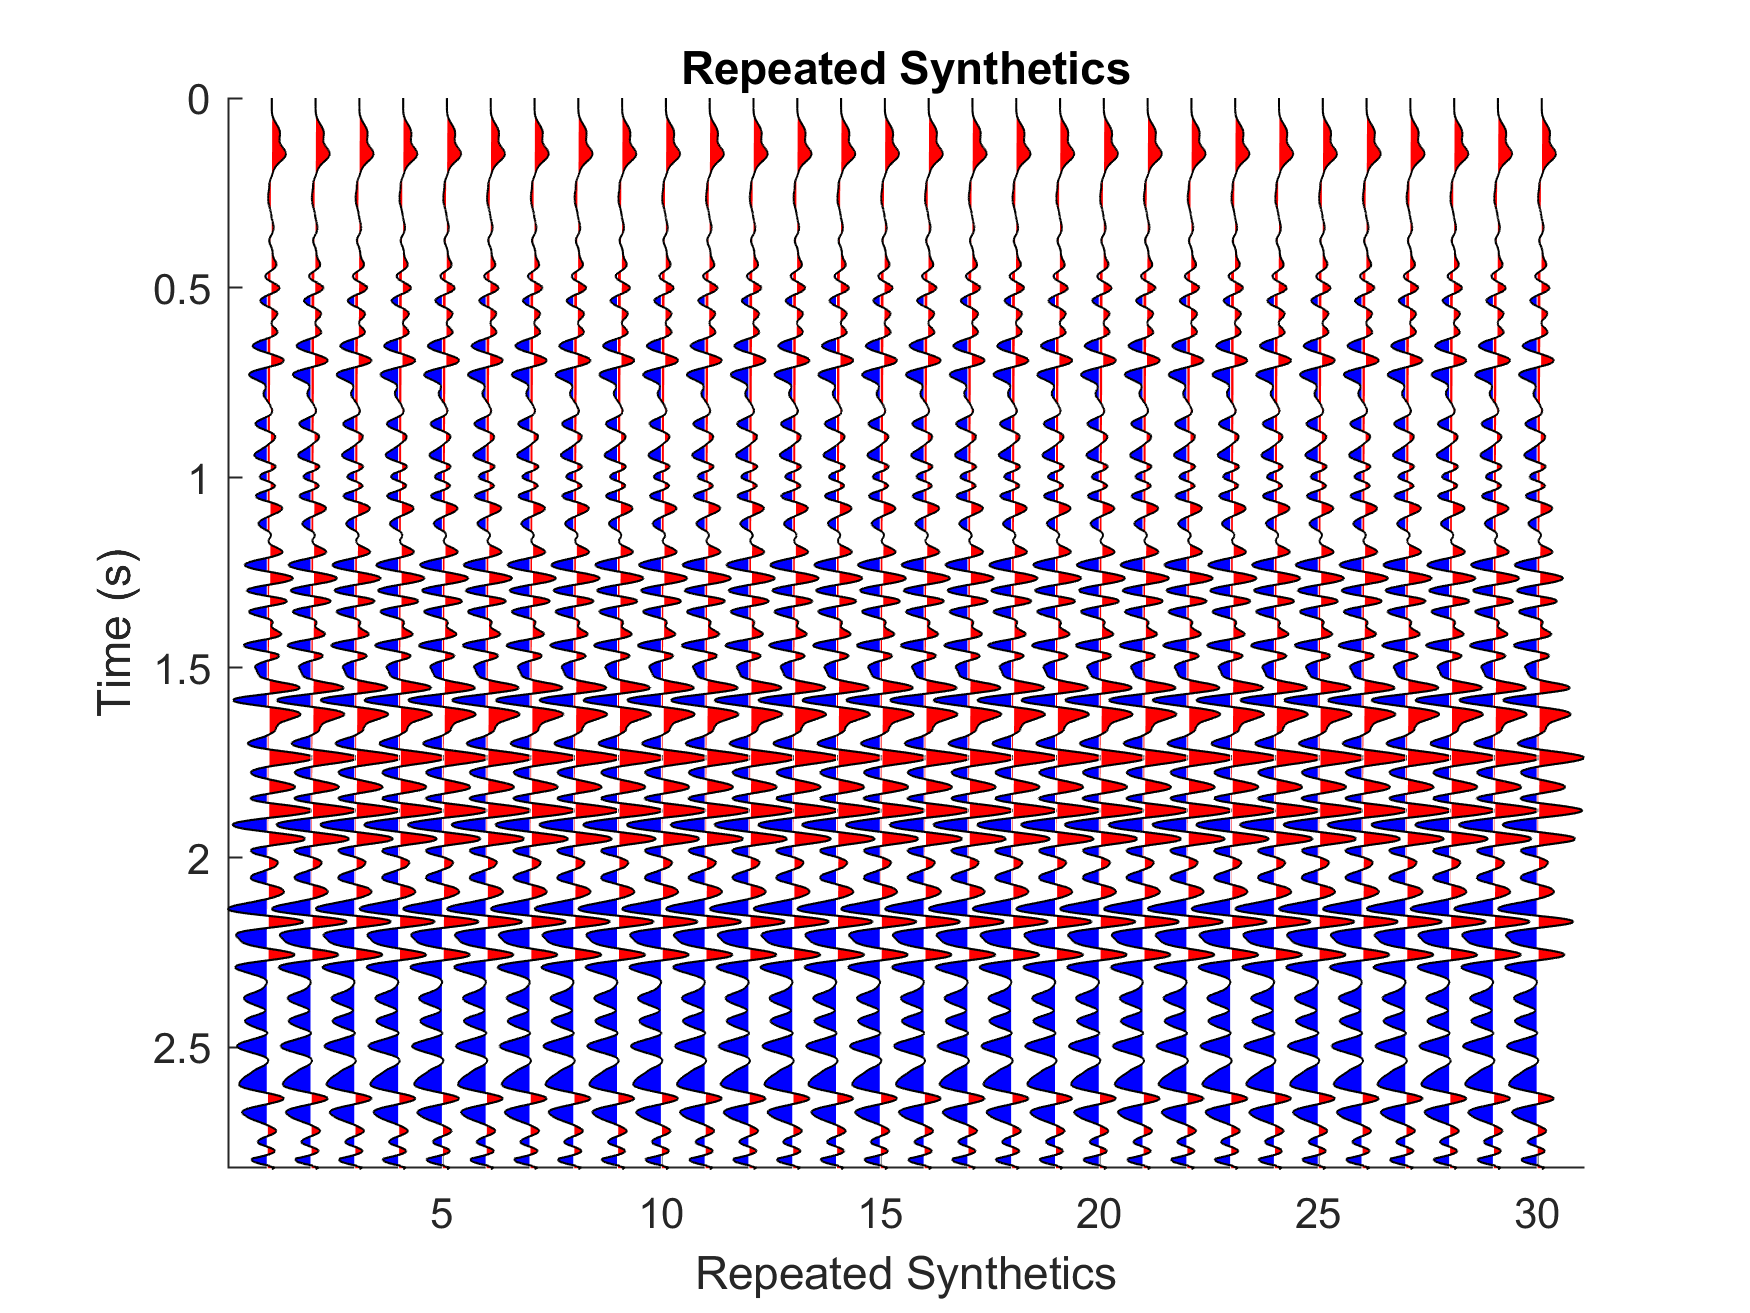
\includegraphics[width=0.7\textwidth]{Figures/FDCseveralstack.png}
	\caption[Fox Creek ray-tracing several P-S synthetic seismograms]{Several synthetic seismograms for P-S reflections from ray-tracing}
	\label{fig:FDCSeveralStack}
\end{figure}
\FloatBarrier
\pagebreak
\subsection{Fox Creek Ray-Tracing P-S}
\begin{figure}[!htb]
	\centering
	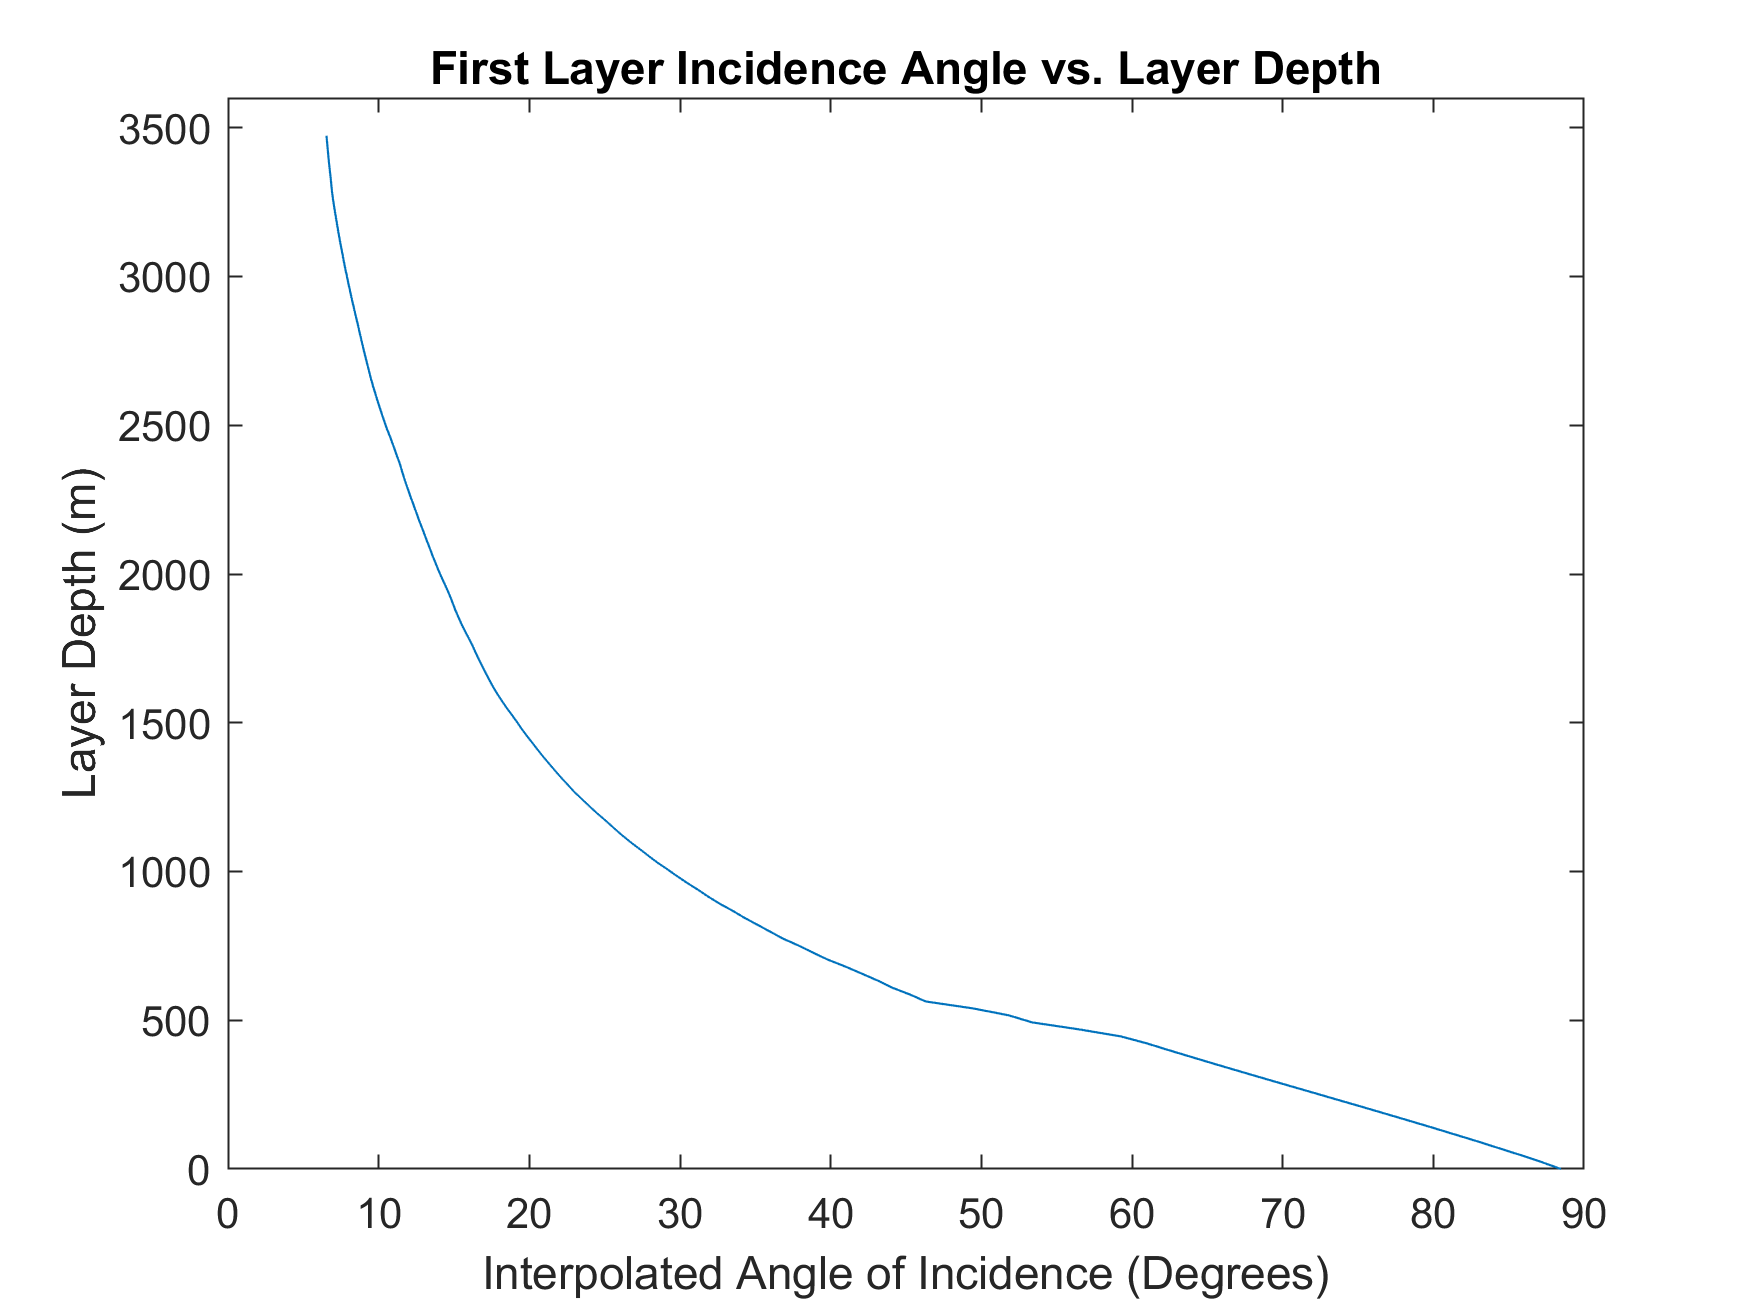
\includegraphics[width=0.7\textwidth]{Figures/RTCDv.png}
	\caption[Fox Creek ray-tracing P-S depth-angle plot]{Layer depth as a function of input angle of incidence for P-S reflections in the Fox Creek region}
	\label{fig:RTCDv}
\end{figure}

\begin{figure}[!htb]
	\centering
	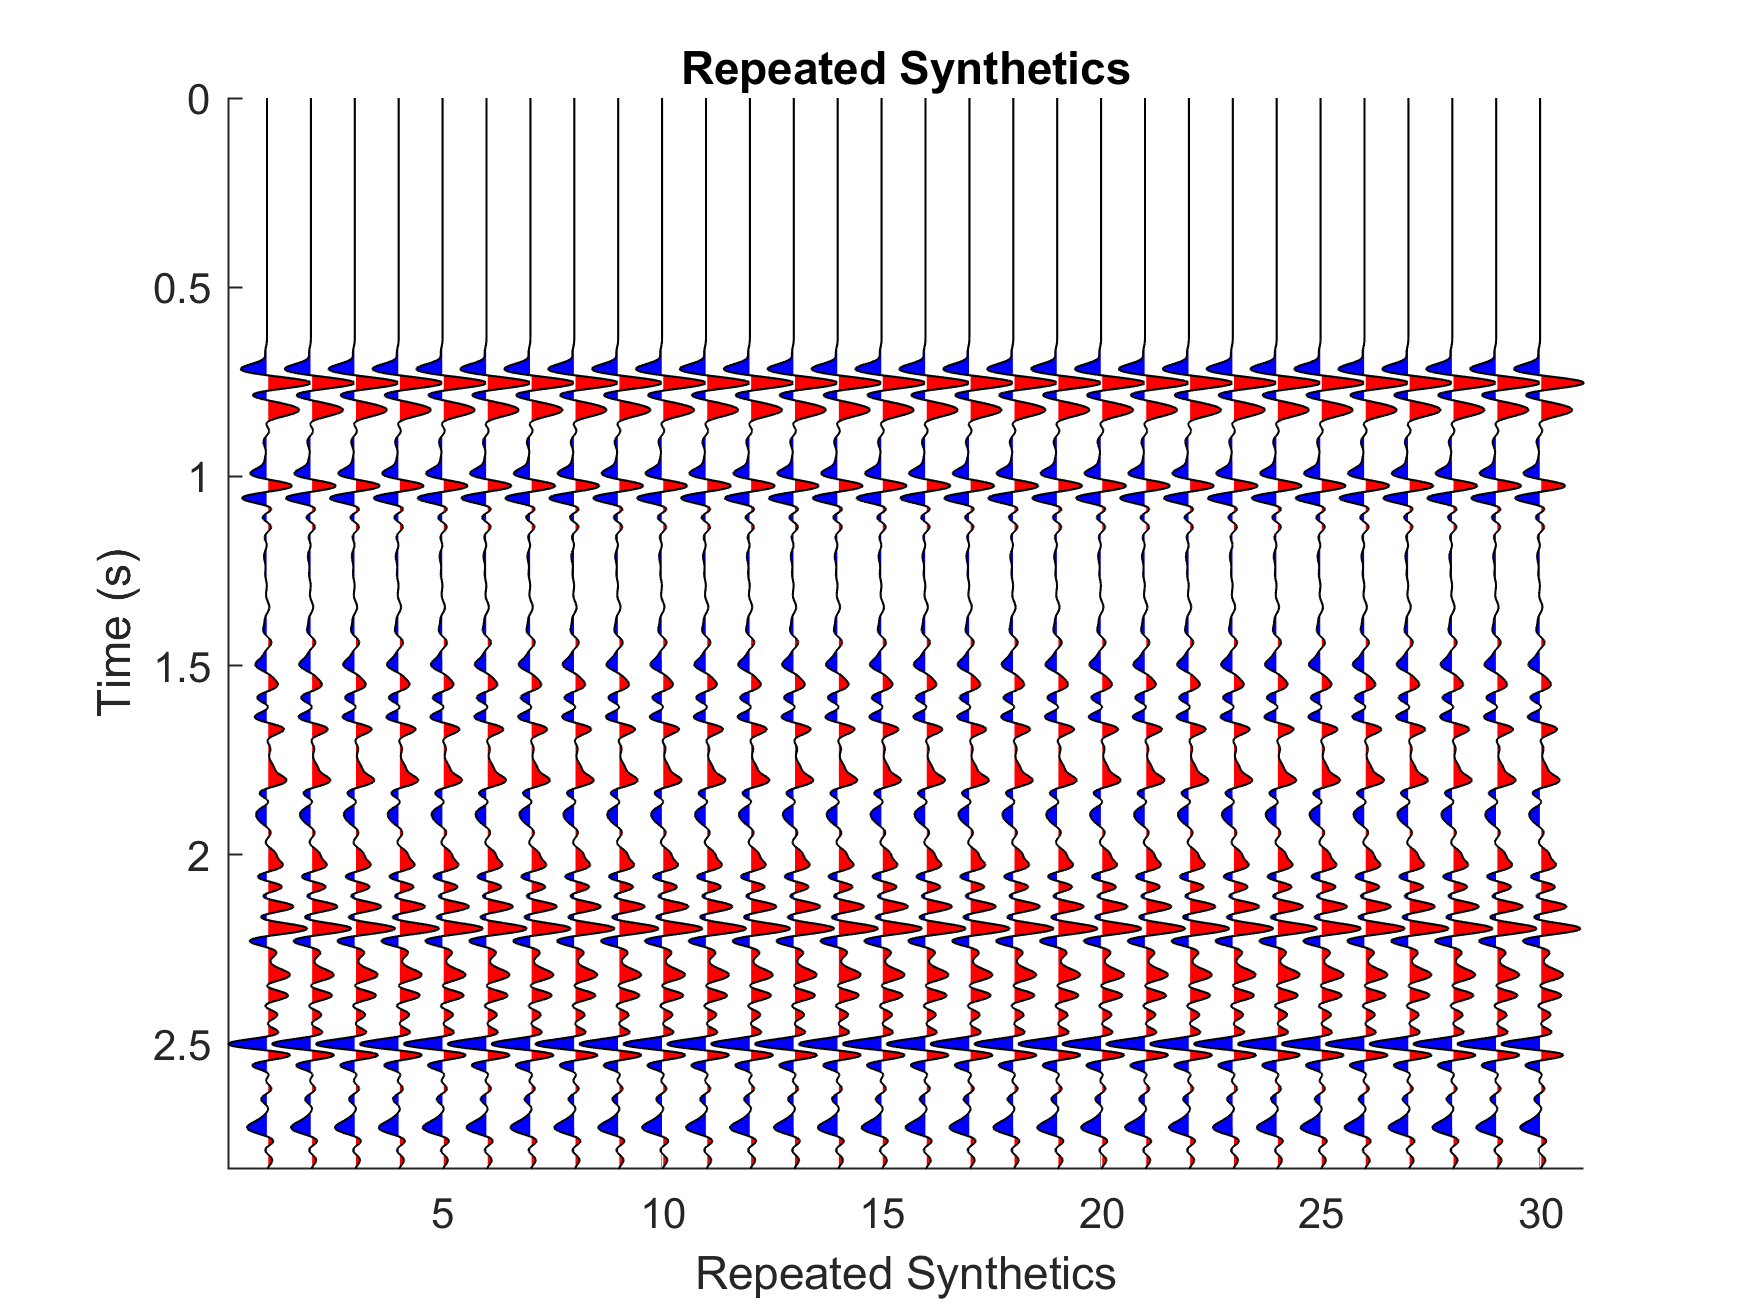
\includegraphics[width=0.7\textwidth]{Figures/RTCSeveralSynthetics.png}
	\caption[Fox Creek ray-tracing several P-S synthetic seismograms]{Several synthetic seismograms for P-S reflections from ray-tracing}
	\label{fig:RTCSeveralSynthetics}
\end{figure}
\FloatBarrier
\pagebreak
\subsection{Fox Creek Finite-Difference P-P}

\begin{figure}[!htb]
	\centering
	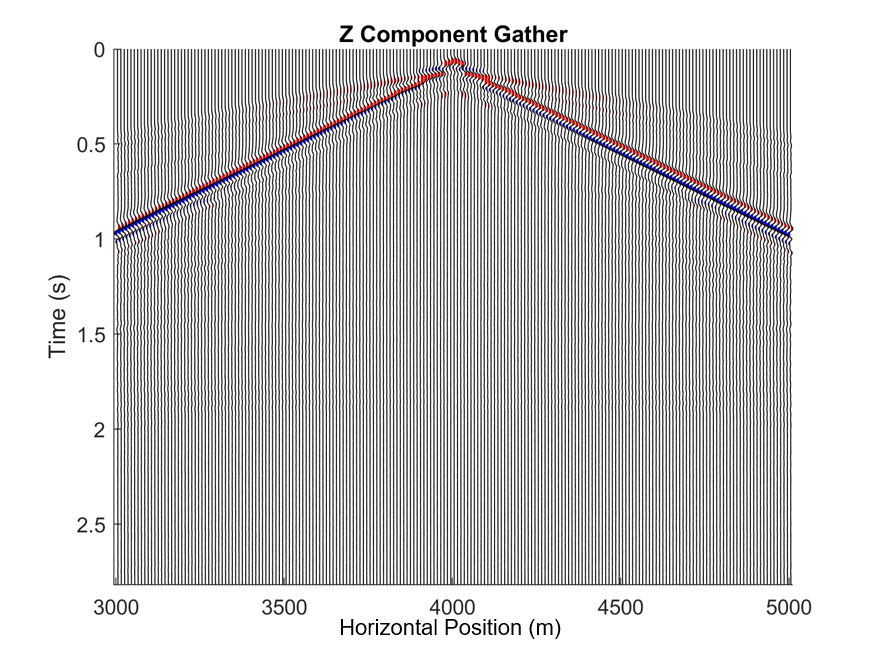
\includegraphics[width=0.7\textwidth]{Figures/FDCZgather.png}
	\caption[Fox Creek finite-difference P-P gather]{Uncorrected P-P output gather from the finite-difference tool}
	\label{fig:FDCZgather}
\end{figure}

\begin{figure}[!htb]
	\centering
	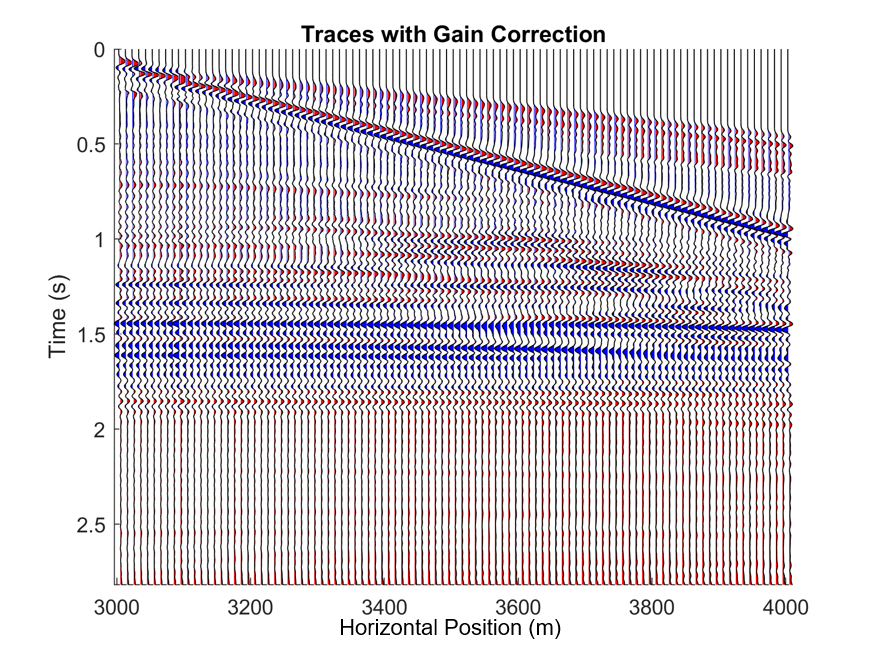
\includegraphics[width=0.7\textwidth]{Figures/FDCgainPP.png}
	\caption[Fox Creek finite-difference P-P gain correction]{Gain corrected Fox Creek data from finite-difference P-P modelling}
	\label{fig:FDCgainPP}
\end{figure}	

\begin{figure}[!htb]
	\centering
	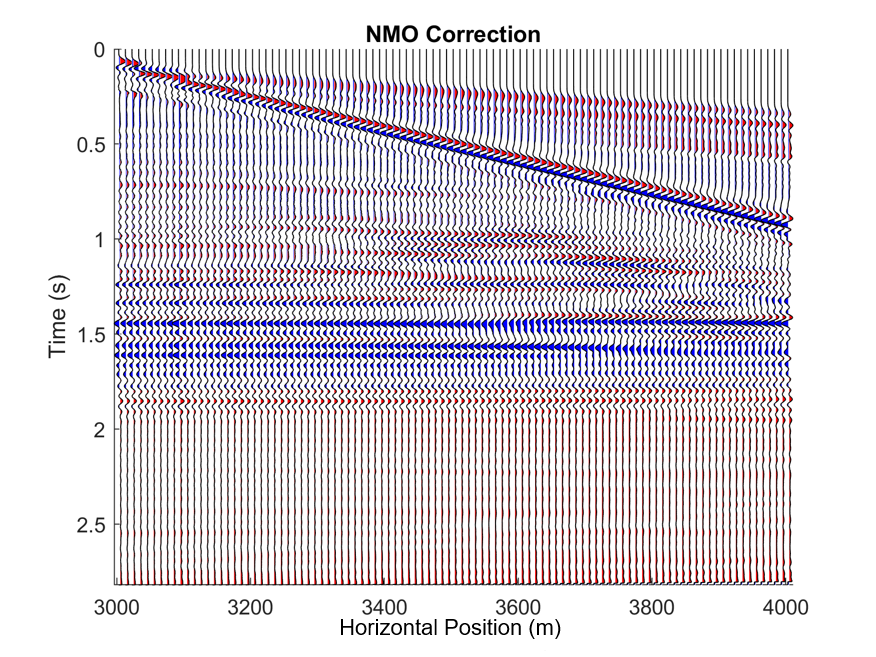
\includegraphics[width=0.7\textwidth]{Figures/FDCnmoPP.png}
	\caption[Fox Creek finite-difference P-P NMO correction]{Velocity corrected Fox Creek data from finite-difference P-P modelling}
	\label{fig:FDCnmoPP}
\end{figure}	

\begin{figure}[!htb]
	\centering
	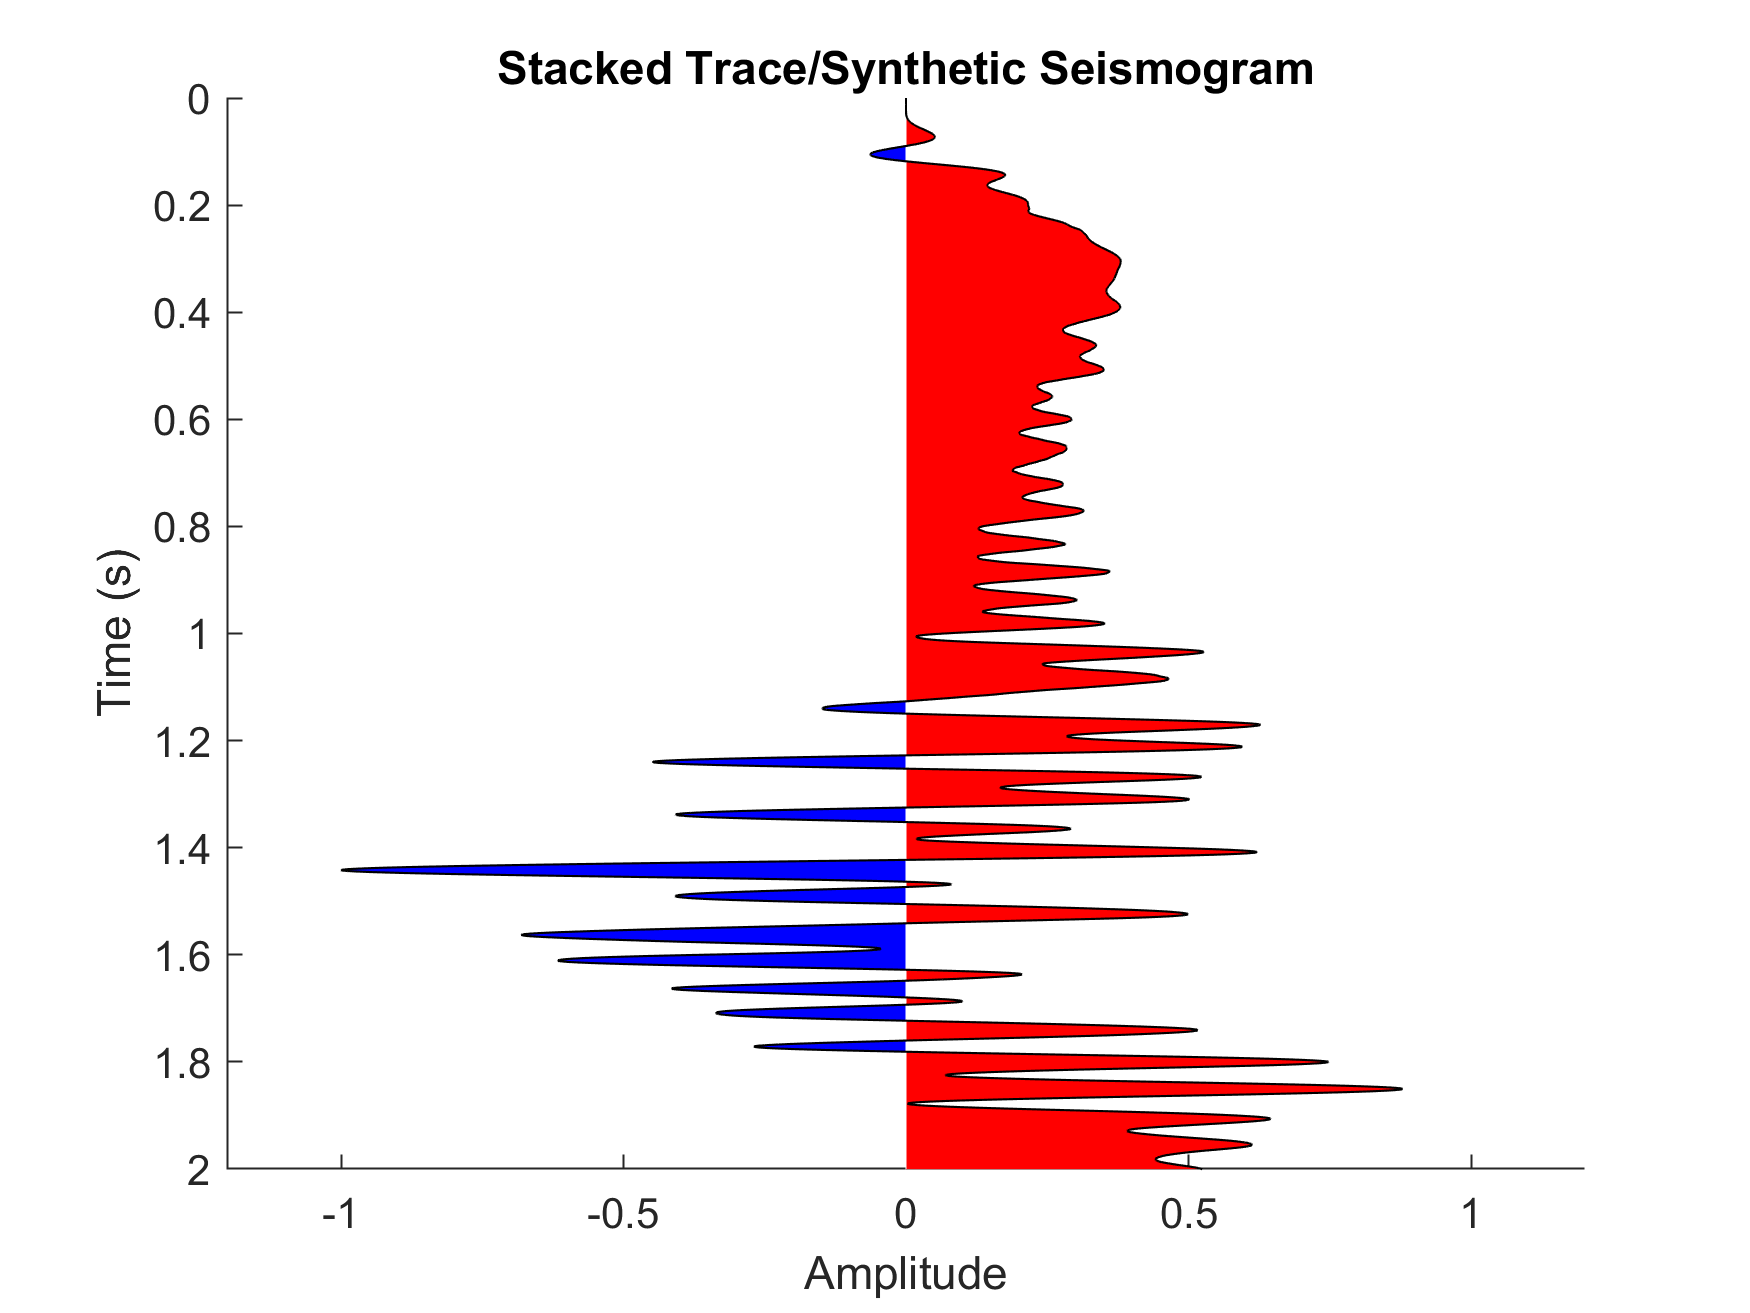
\includegraphics[width=0.7\textwidth]{Figures/FDCstackPP.png}
	\caption[Fox Creek finite-difference P-P synthetic seismogram]{Stacked trace and the synthetic seismogram from finite-difference modelling P-P modelling}
	\label{fig:FDCstackPP}
\end{figure}

\begin{figure}[!htb]
	\centering
	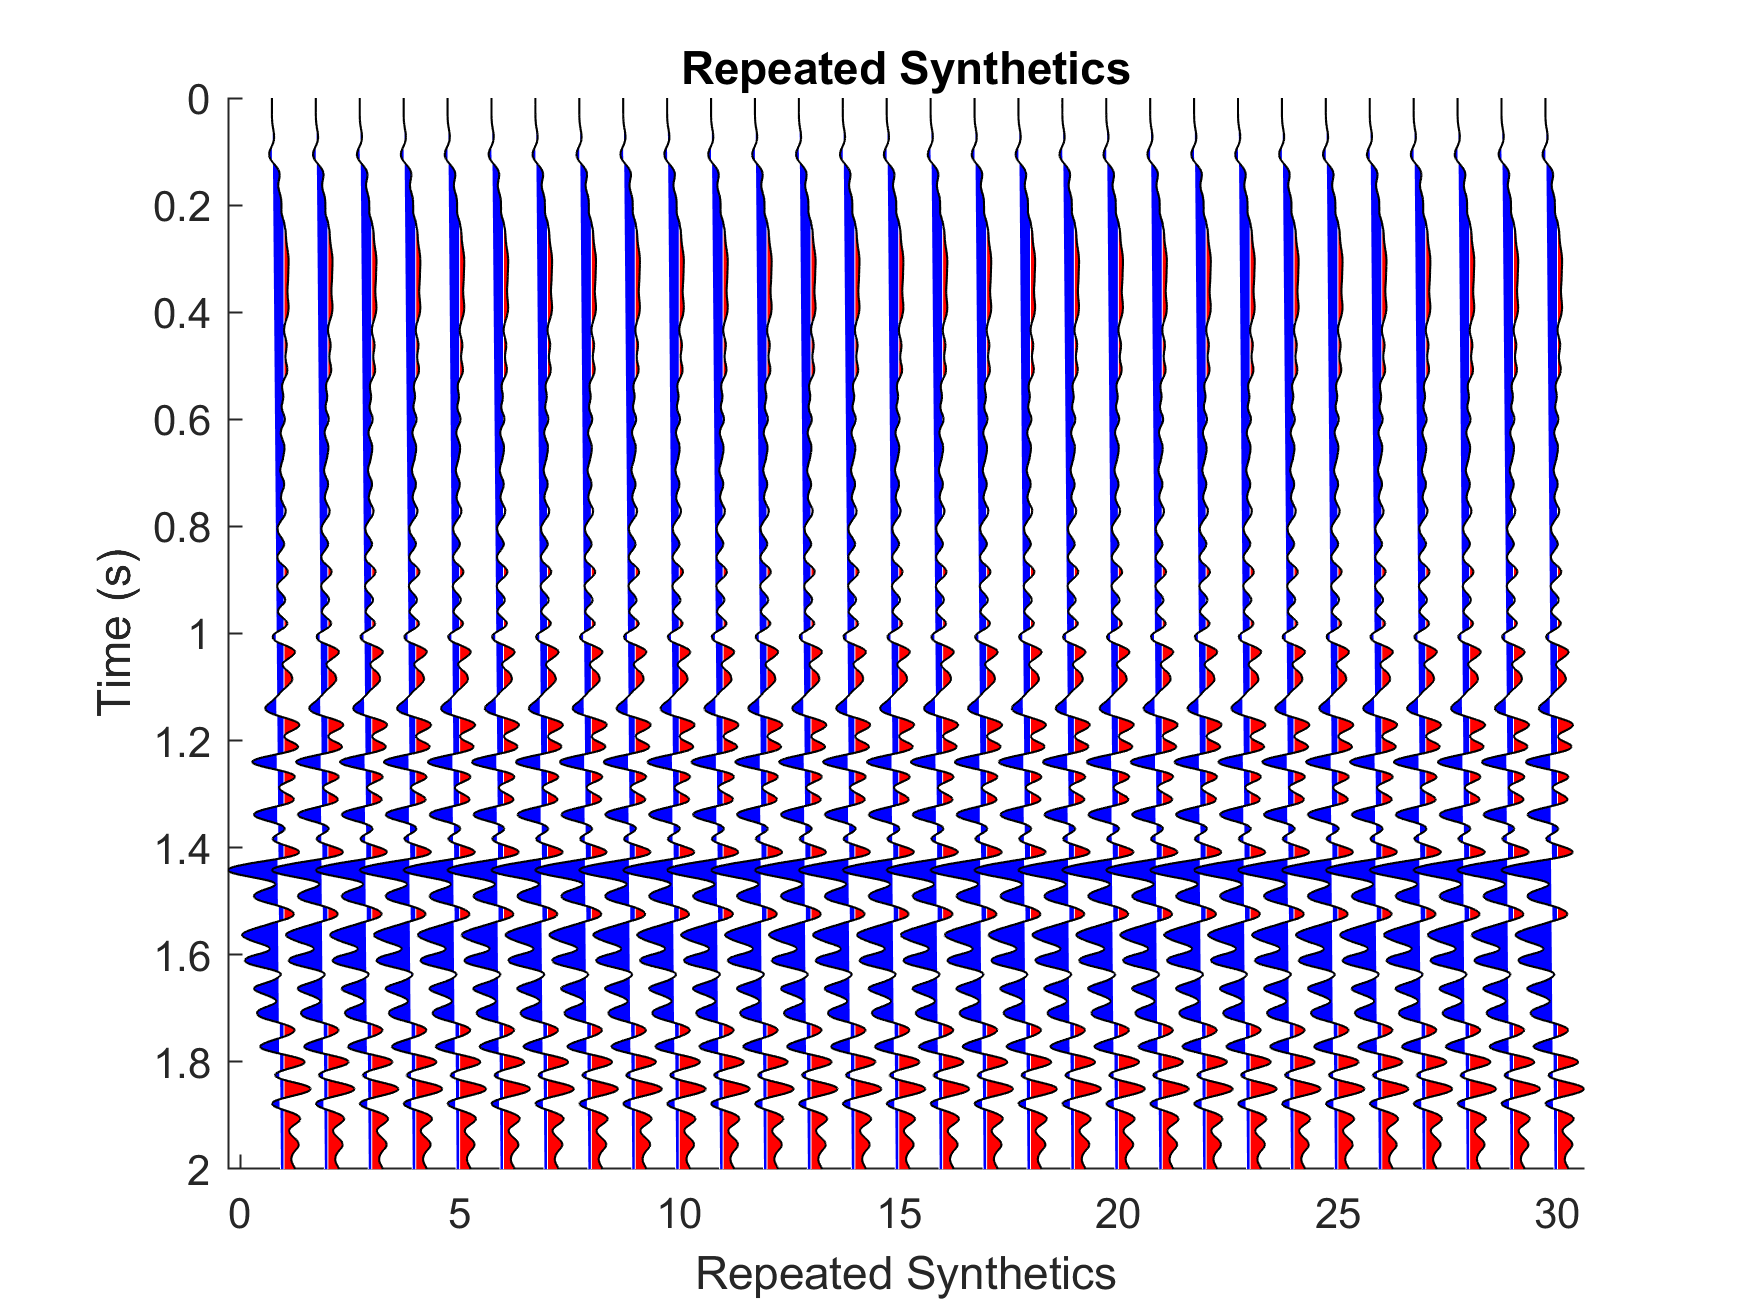
\includegraphics[width=0.7\textwidth]{Figures/FDCseveralstackPP.png}
	\caption[Fox Creek ray-tracing several P-P synthetic seismograms]{Several synthetic seismograms for P-P reflections from ray-tracing}
	\label{fig:FDCSeveralStackPP}
\end{figure}
\FloatBarrier
\pagebreak
\subsection{Fox Creek Ray-Tracing P-P}
\begin{figure}[!htb]
	\centering
	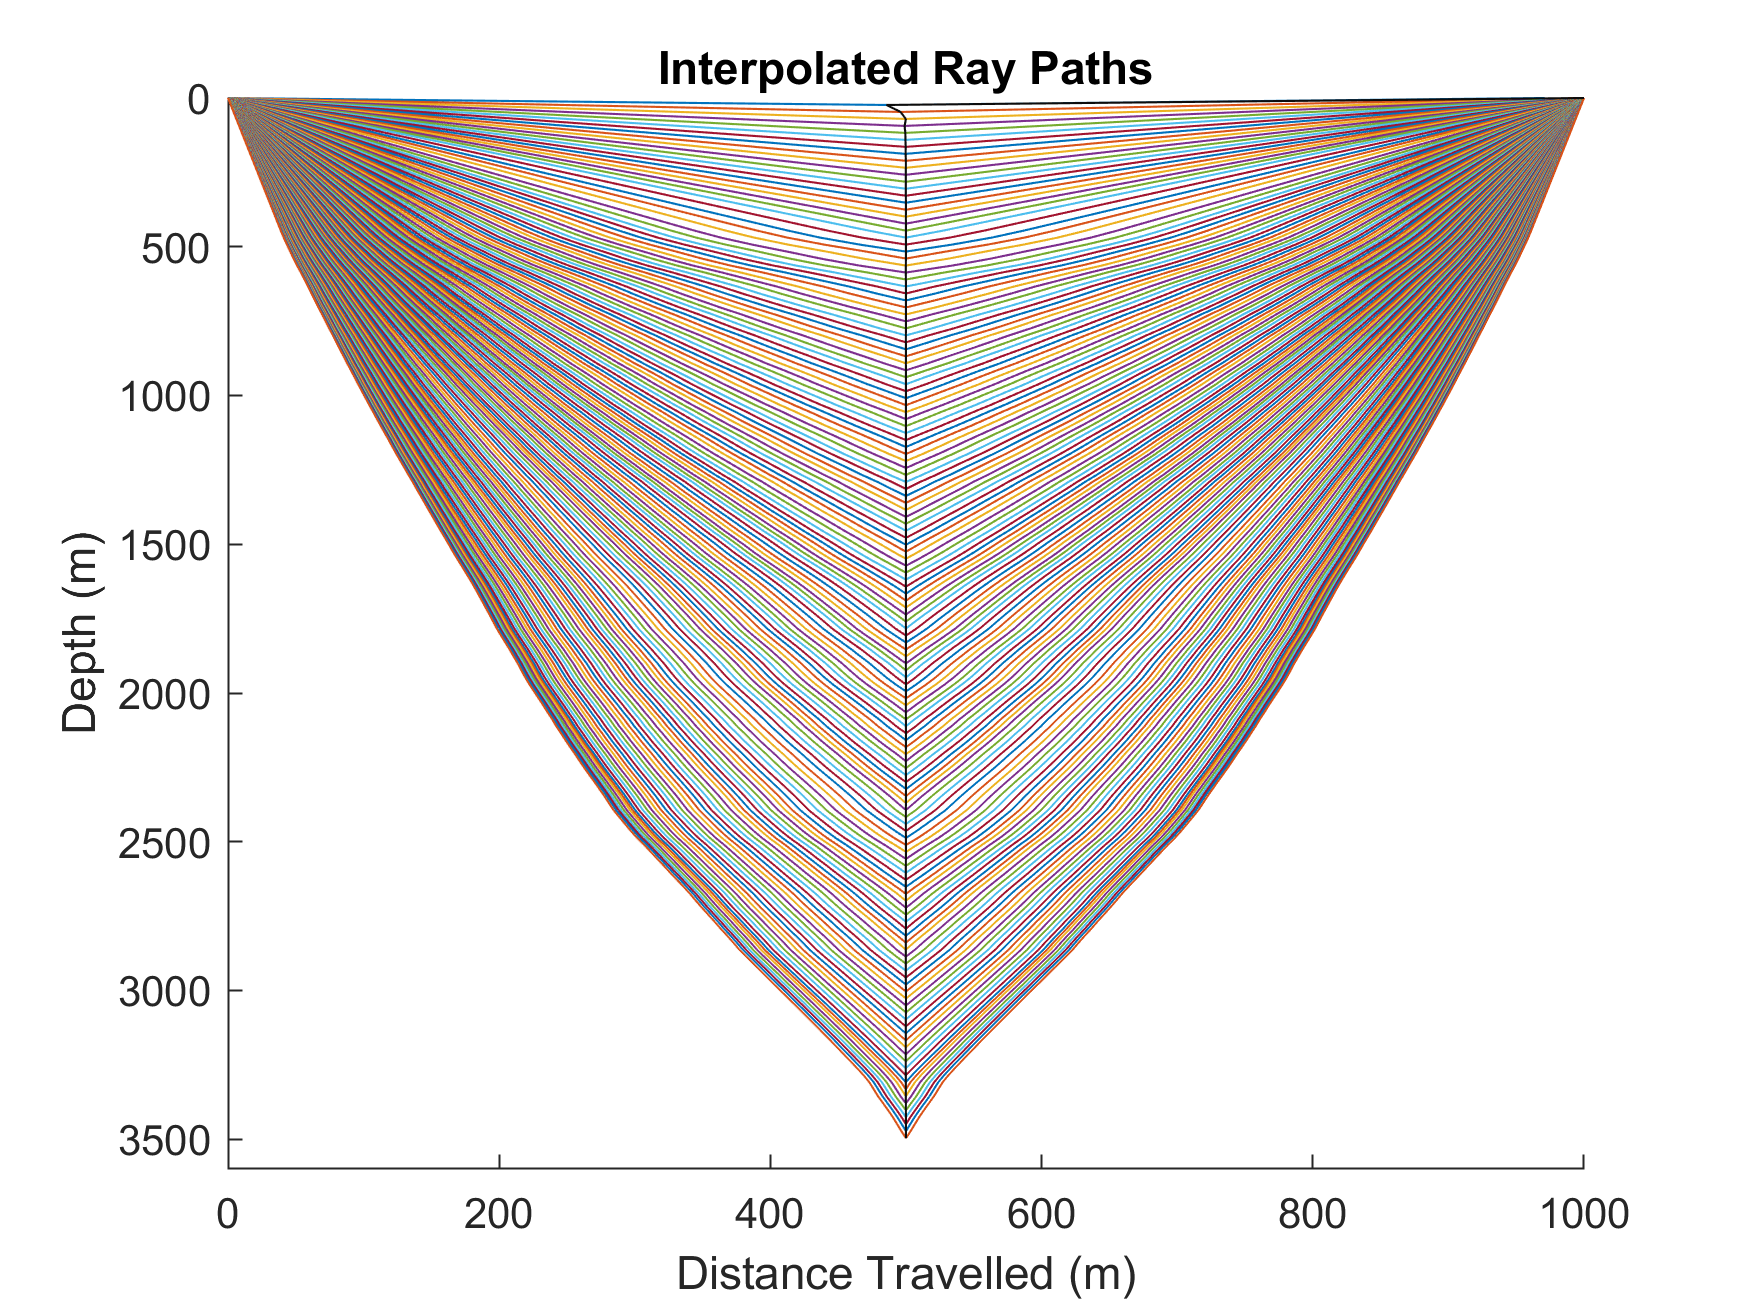
\includegraphics[width=0.7\textwidth]{Figures/RTCinterpPP.png}
	\caption[Fox Creek ray-tracing P-P ray-paths]{Interpolated P-P ray-paths}
	\label{fig:RTCinterpPP}
\end{figure}

\begin{figure}[!htb]
	\centering
	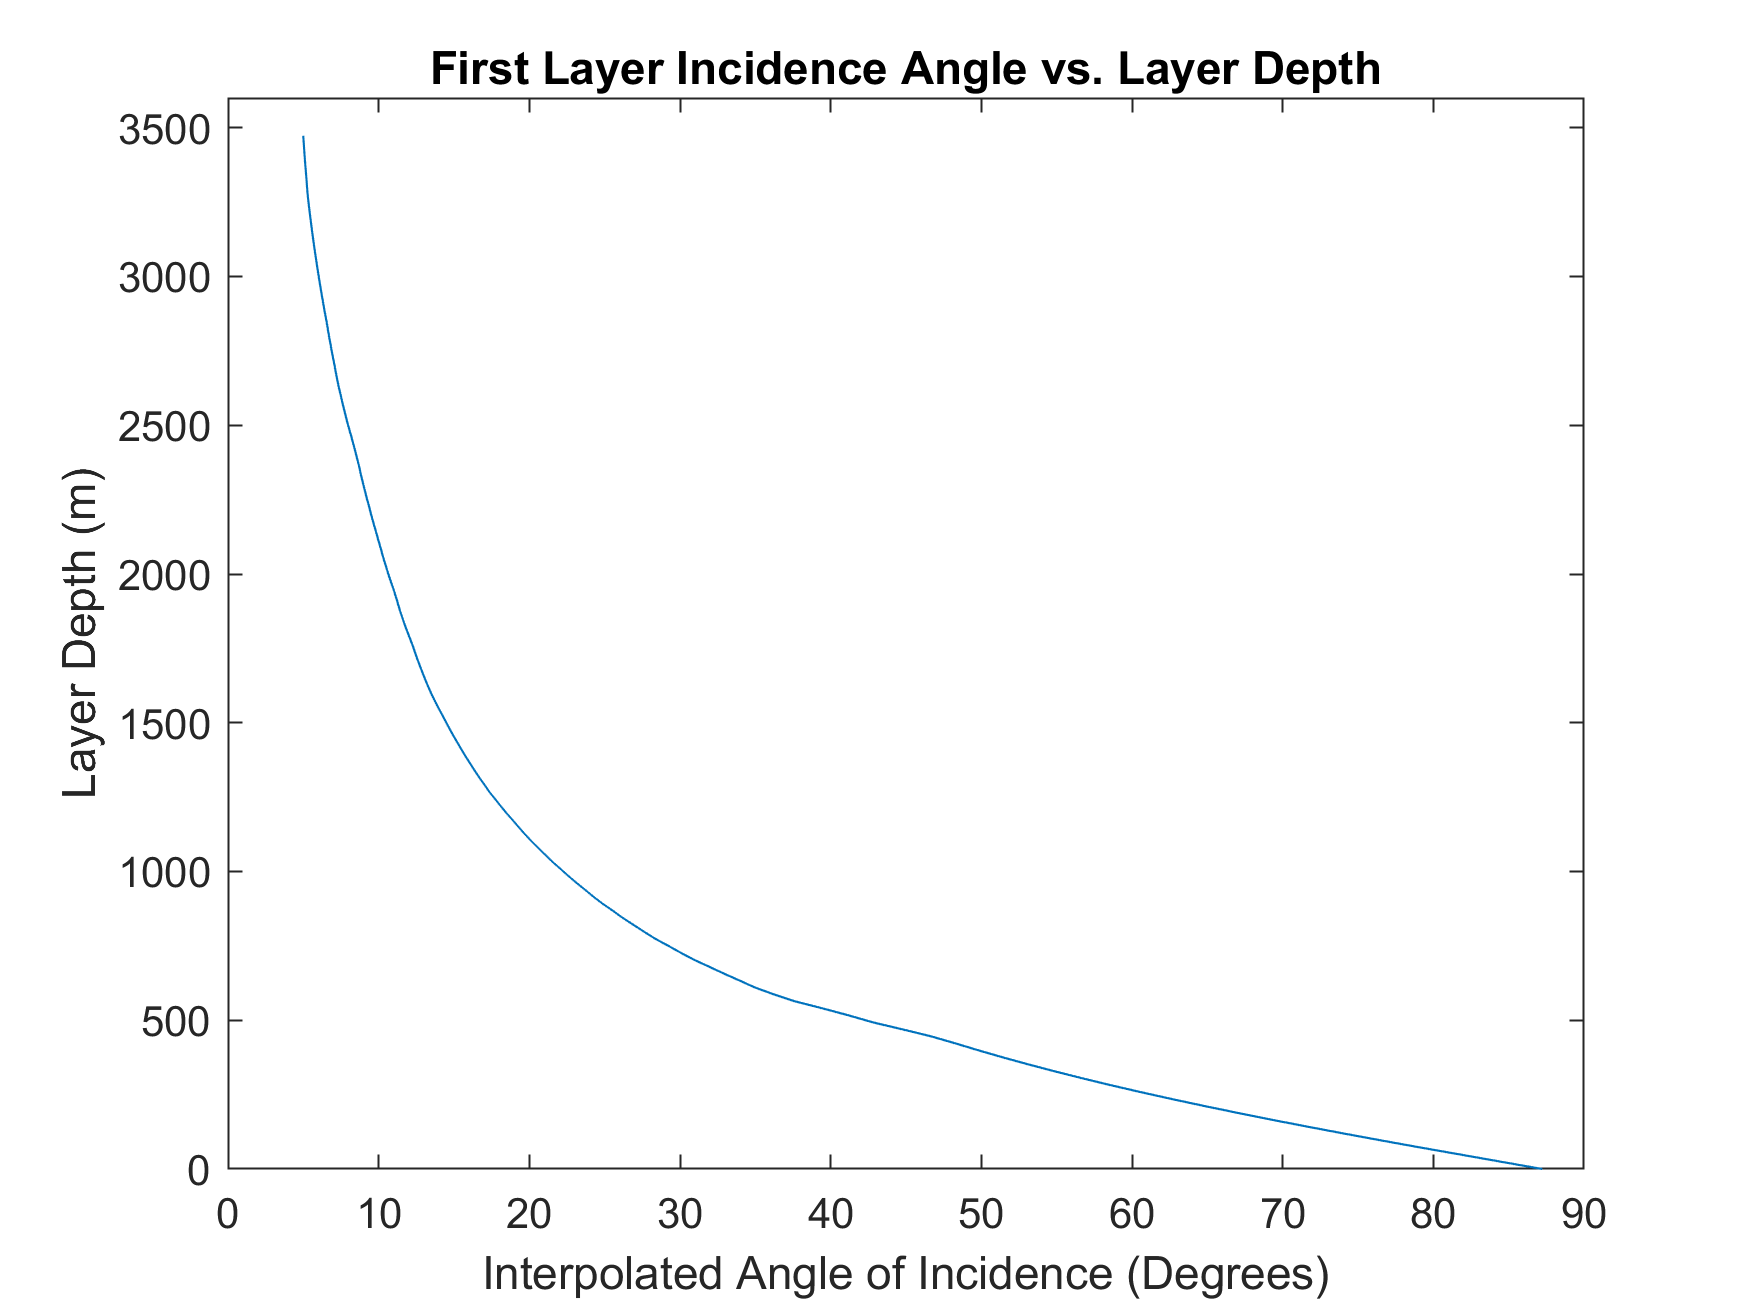
\includegraphics[width=0.7\textwidth]{Figures/RTCDvPP.png}
	\caption[Fox Creek ray-tracing P-P depth-angle plot]{Layer depth as a function of input angle of incidence for P-P reflections in the Fox Creek region}
	\label{fig:RTCDvPP}
\end{figure}

\begin{figure}[!htb]
	\centering
	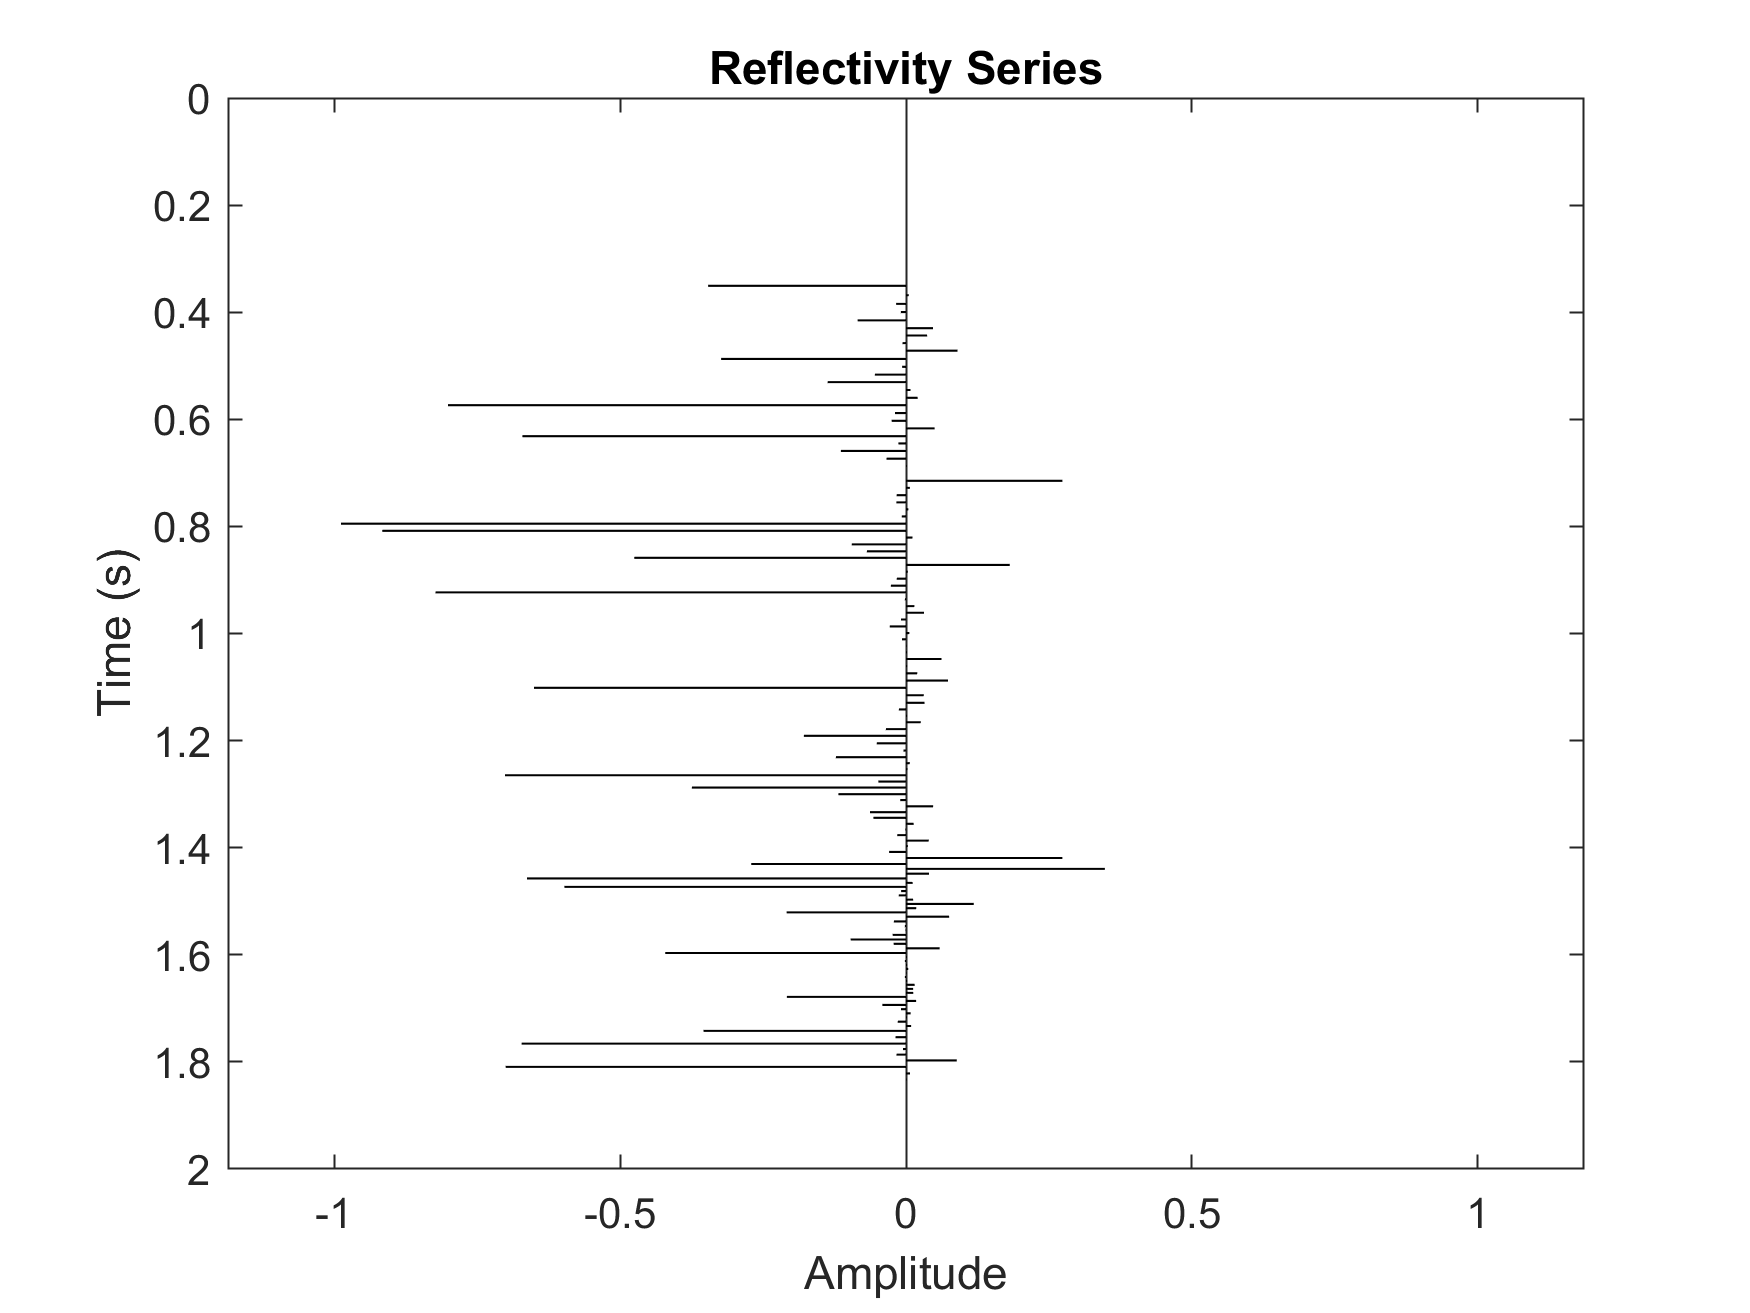
\includegraphics[width=0.7\textwidth]{Figures/RTCrefseriesPP.png}
	\caption[Fox Creek ray-tracing P-P reflectivity series]{Reflectivity Series for P-P reflections from ray-tracing}
	\label{fig:RTCrefseriesPP}
\end{figure}	

\begin{figure}[!htb]
	\centering
	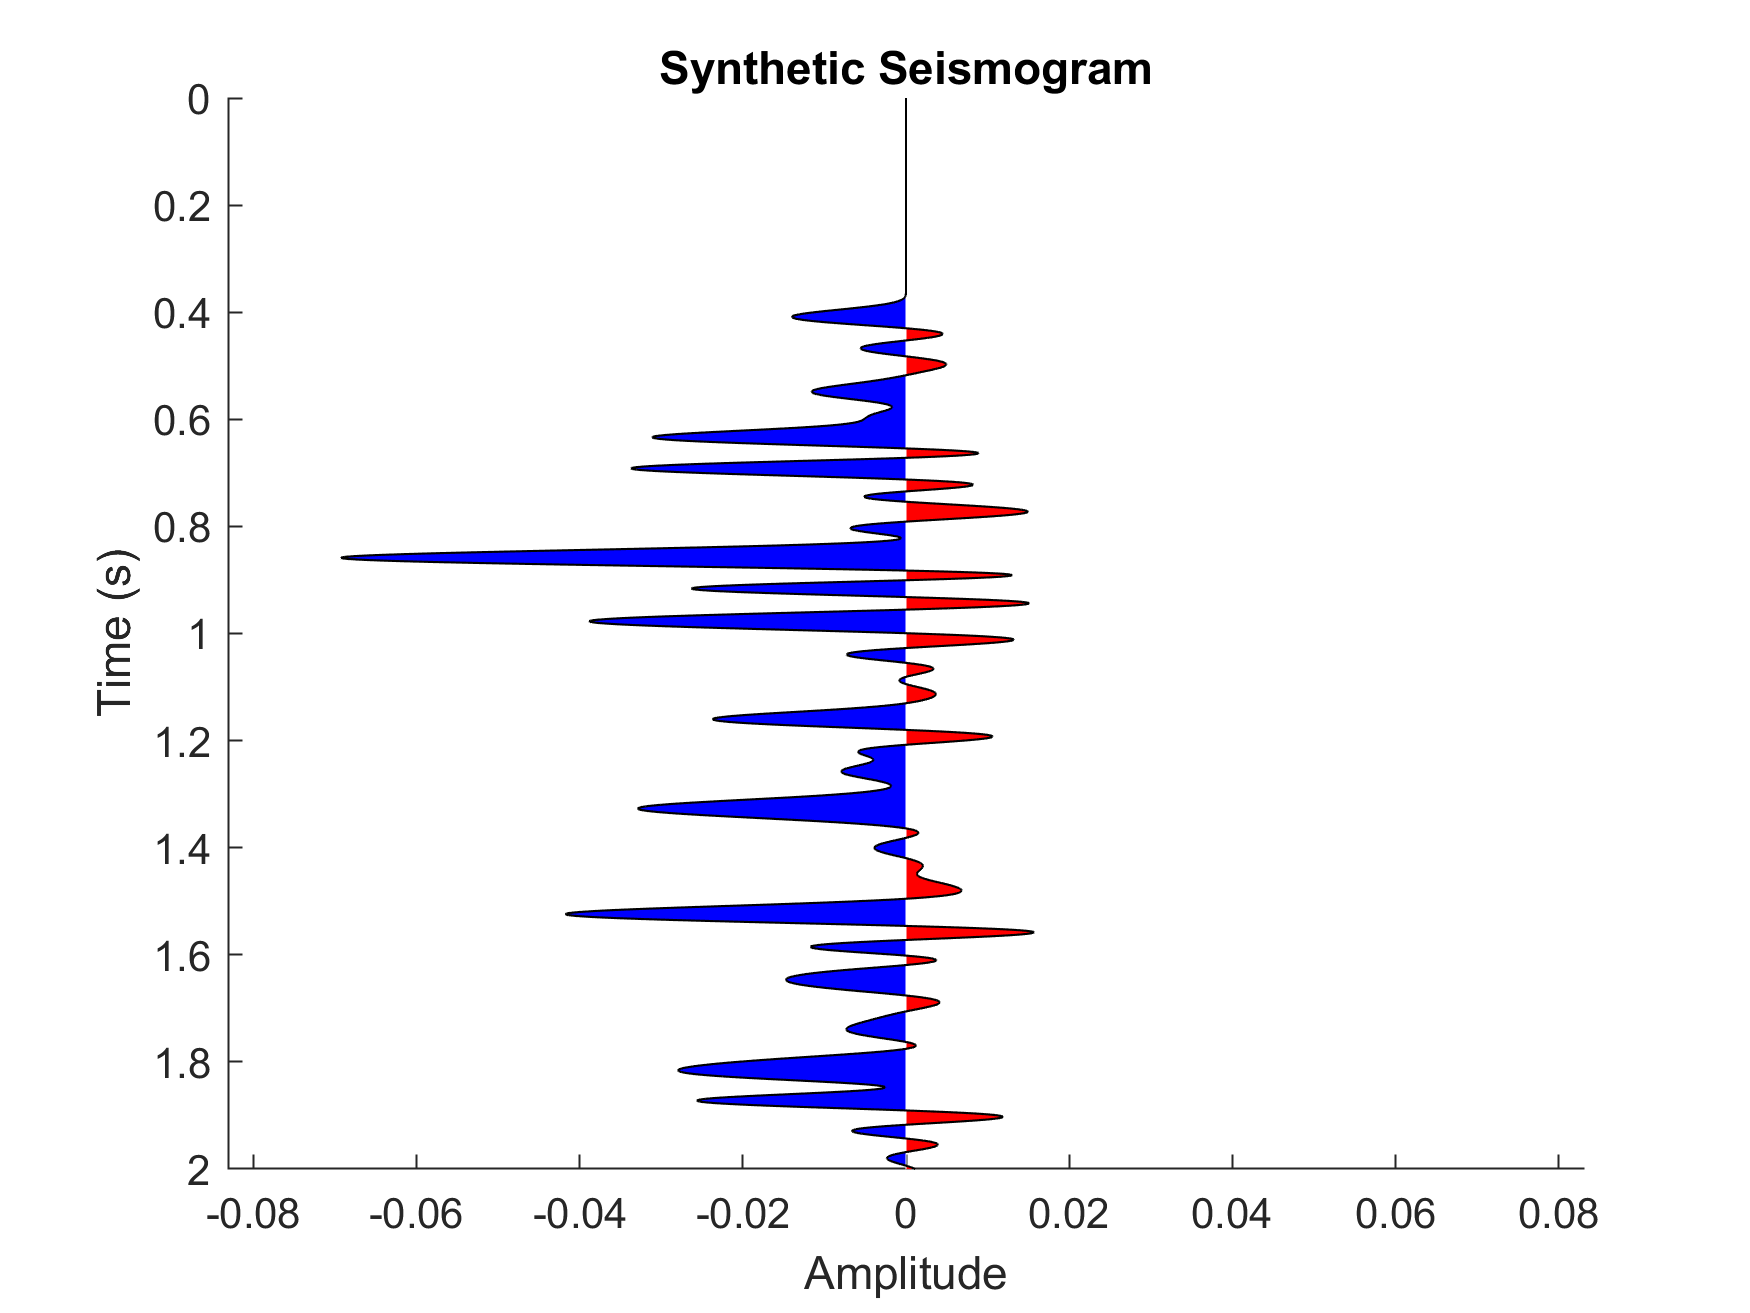
\includegraphics[width=0.7\textwidth]{Figures/RTCsyntheticPP.png}
	\caption[Fox Creek ray-tracing P-P synthetic seismogram]{Synthetic seismogram for P-P reflections from ray-tracing}
	\label{fig:RTCsyntheticPP}
\end{figure}	

\begin{figure}[!htb]
	\centering
	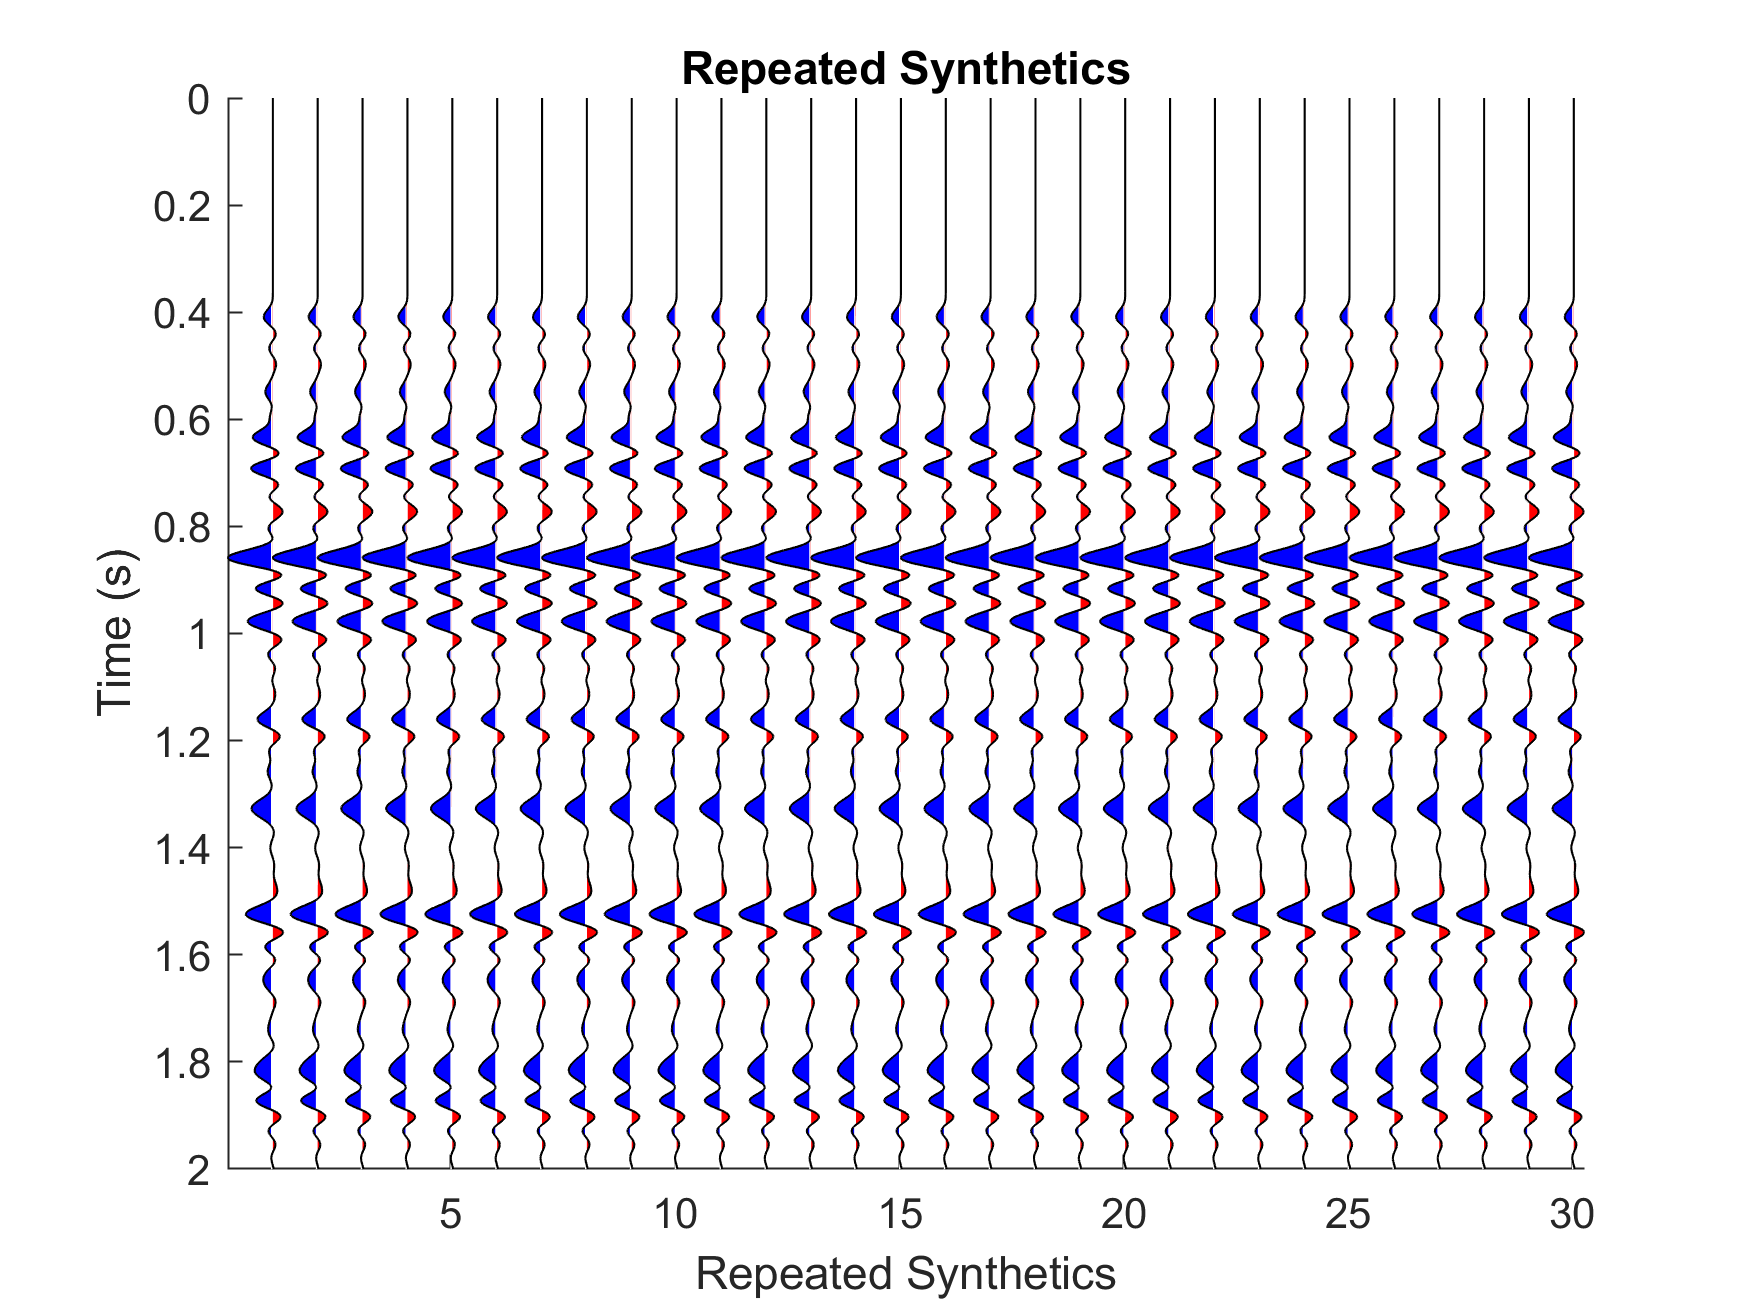
\includegraphics[width=0.7\textwidth]{Figures/RTCSeveralSyntheticsPP.png}
	\caption[Fox Creek ray-tracing several P-P synthetic seismograms]{Several synthetic seismograms for P-P reflections from ray-tracing}
	\label{fig:RTCSeveralSyntheticsPP}
\end{figure}	

\begin{figure}[!htb]
	\centering
	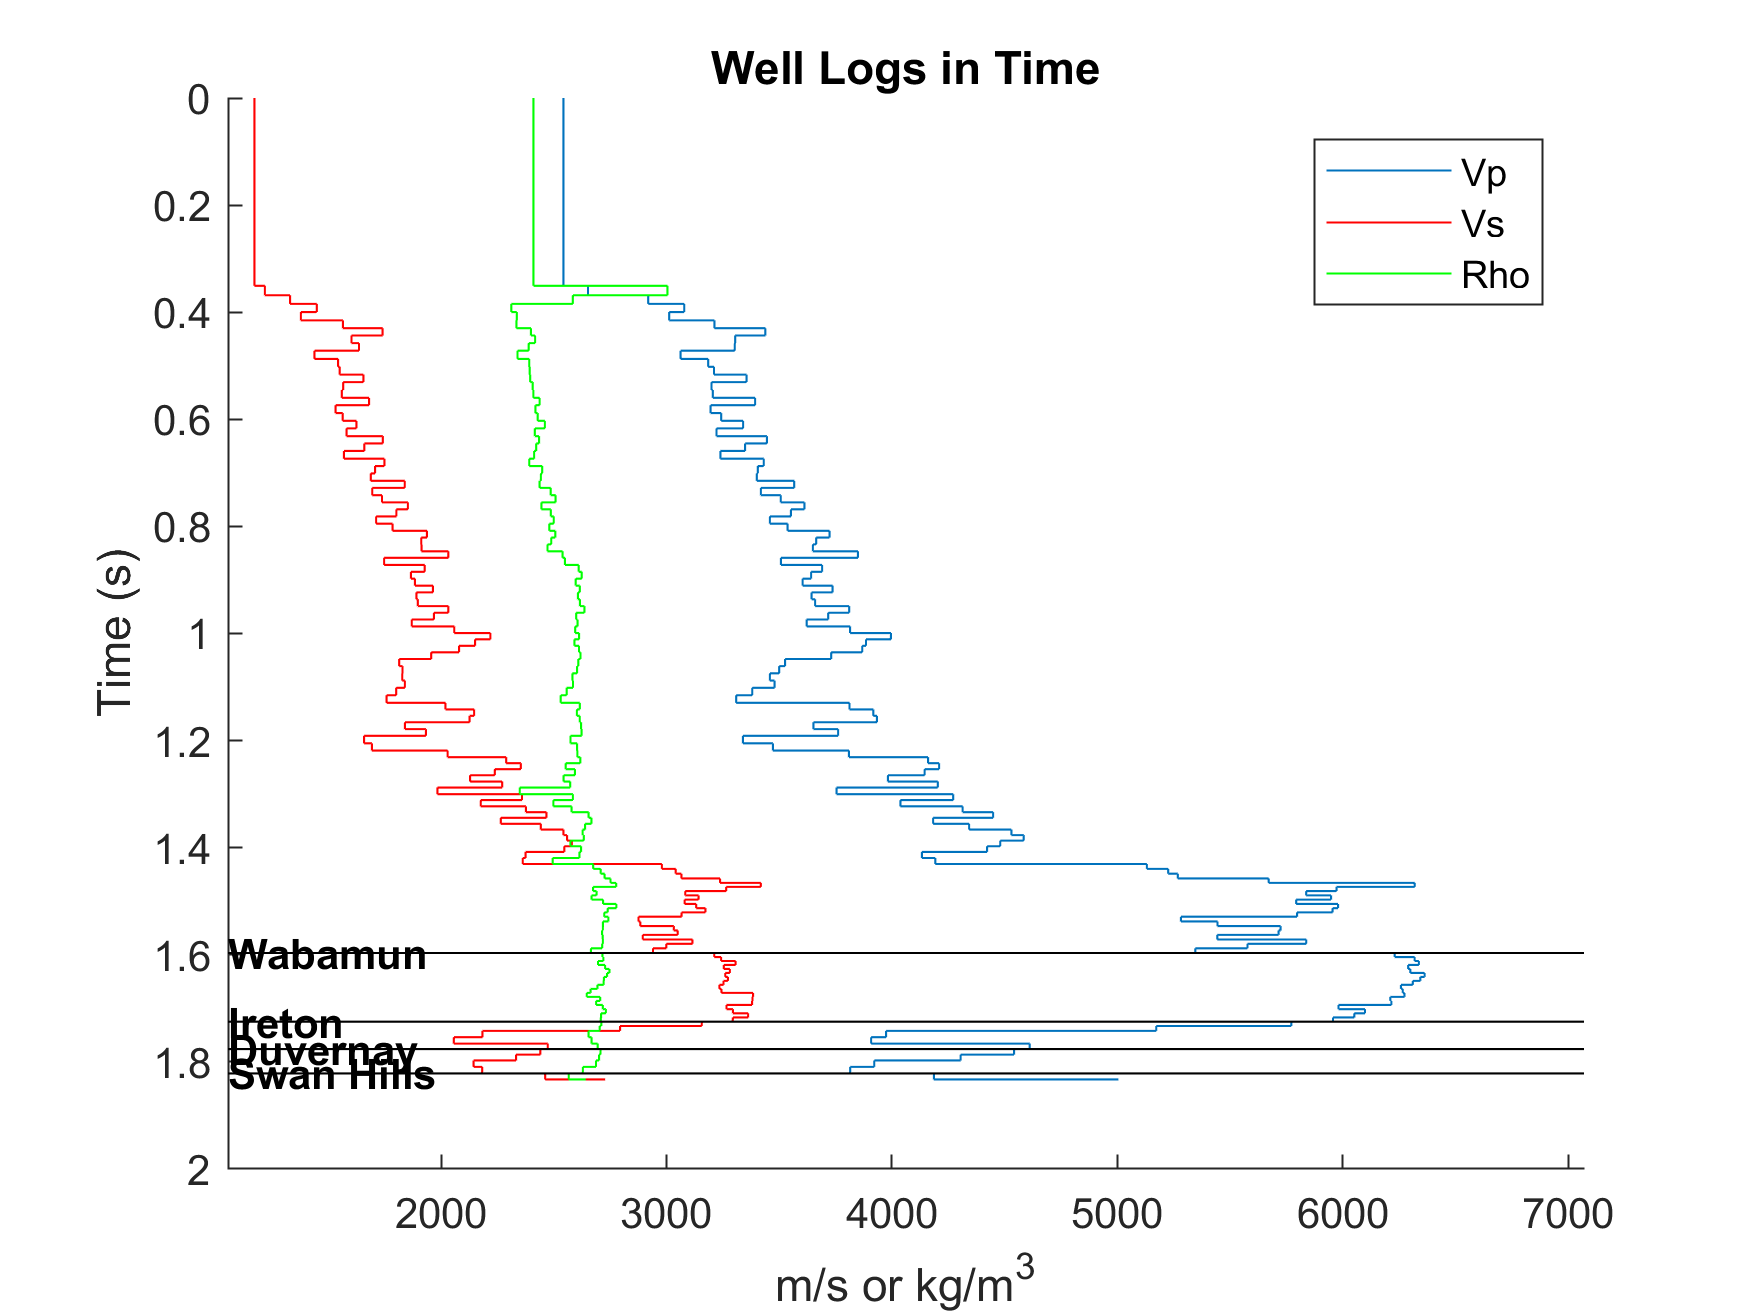
\includegraphics[width=0.7\textwidth]{Figures/RTCtimelogsPP.png}
	\caption[Fox Creek ray-tracing P-P well logs in time]{Well logs converted from depth to time using the time-depth-relationship from P-P reflections}
	\label{fig:RTCtimelogsPP}
\end{figure}
\FloatBarrier

\subsection{Fox Creek Ray-Tracing P-P (Ricker Wavelet)}
\begin{figure}[!htb]
	\centering
	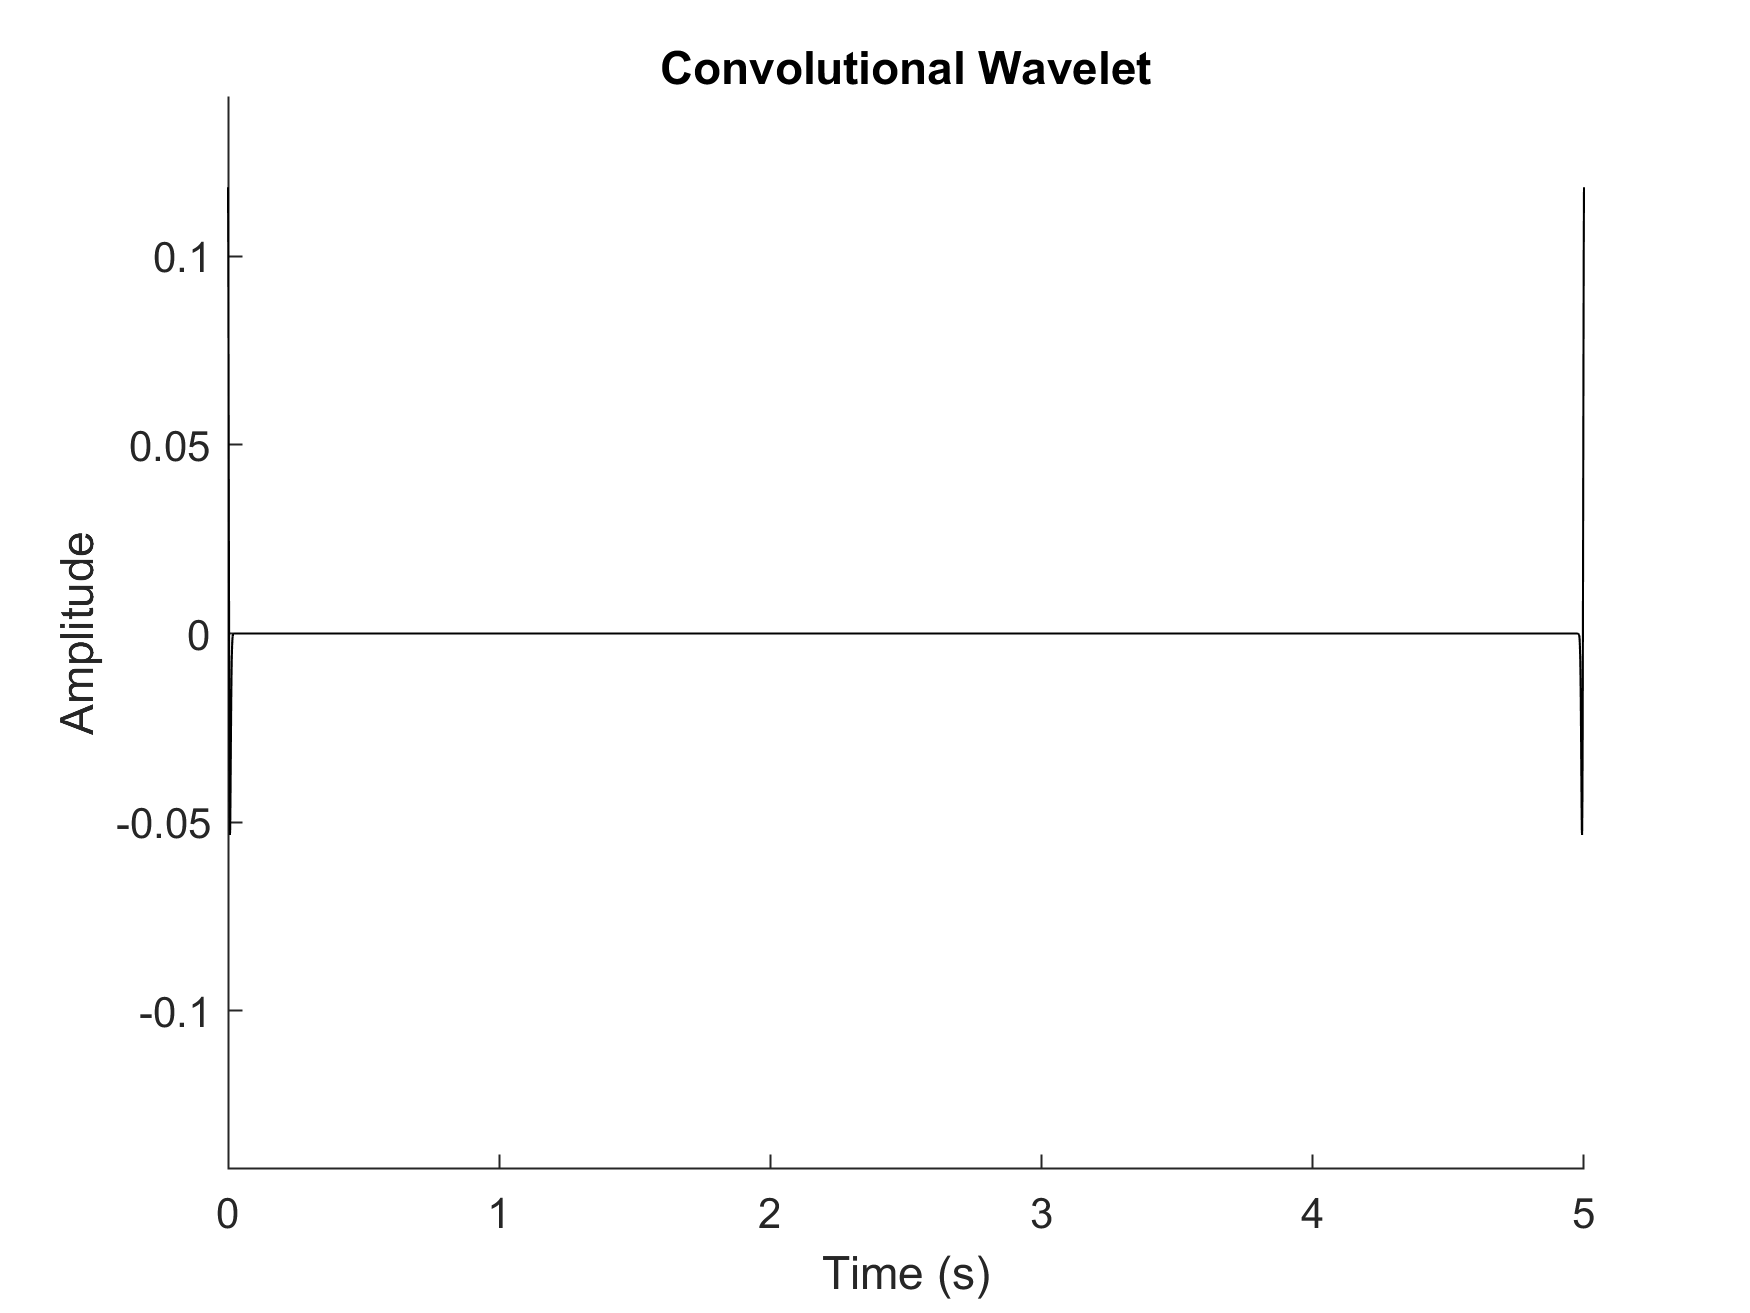
\includegraphics[width=0.7\textwidth]{Figures/RTCricker.png}
	\caption[Fox Creek Ricker wavelet]{$20 Hz$ zero-phase Ricker wavelet used in the shift-and-sum convolution method for ray-tracing. The amplitudes that have 'negative time' are wrapped around to the end of the time signature set for the wavelet.}
	\label{fig:RTCricker}
\end{figure}

\begin{figure}[!htb]
	\centering
	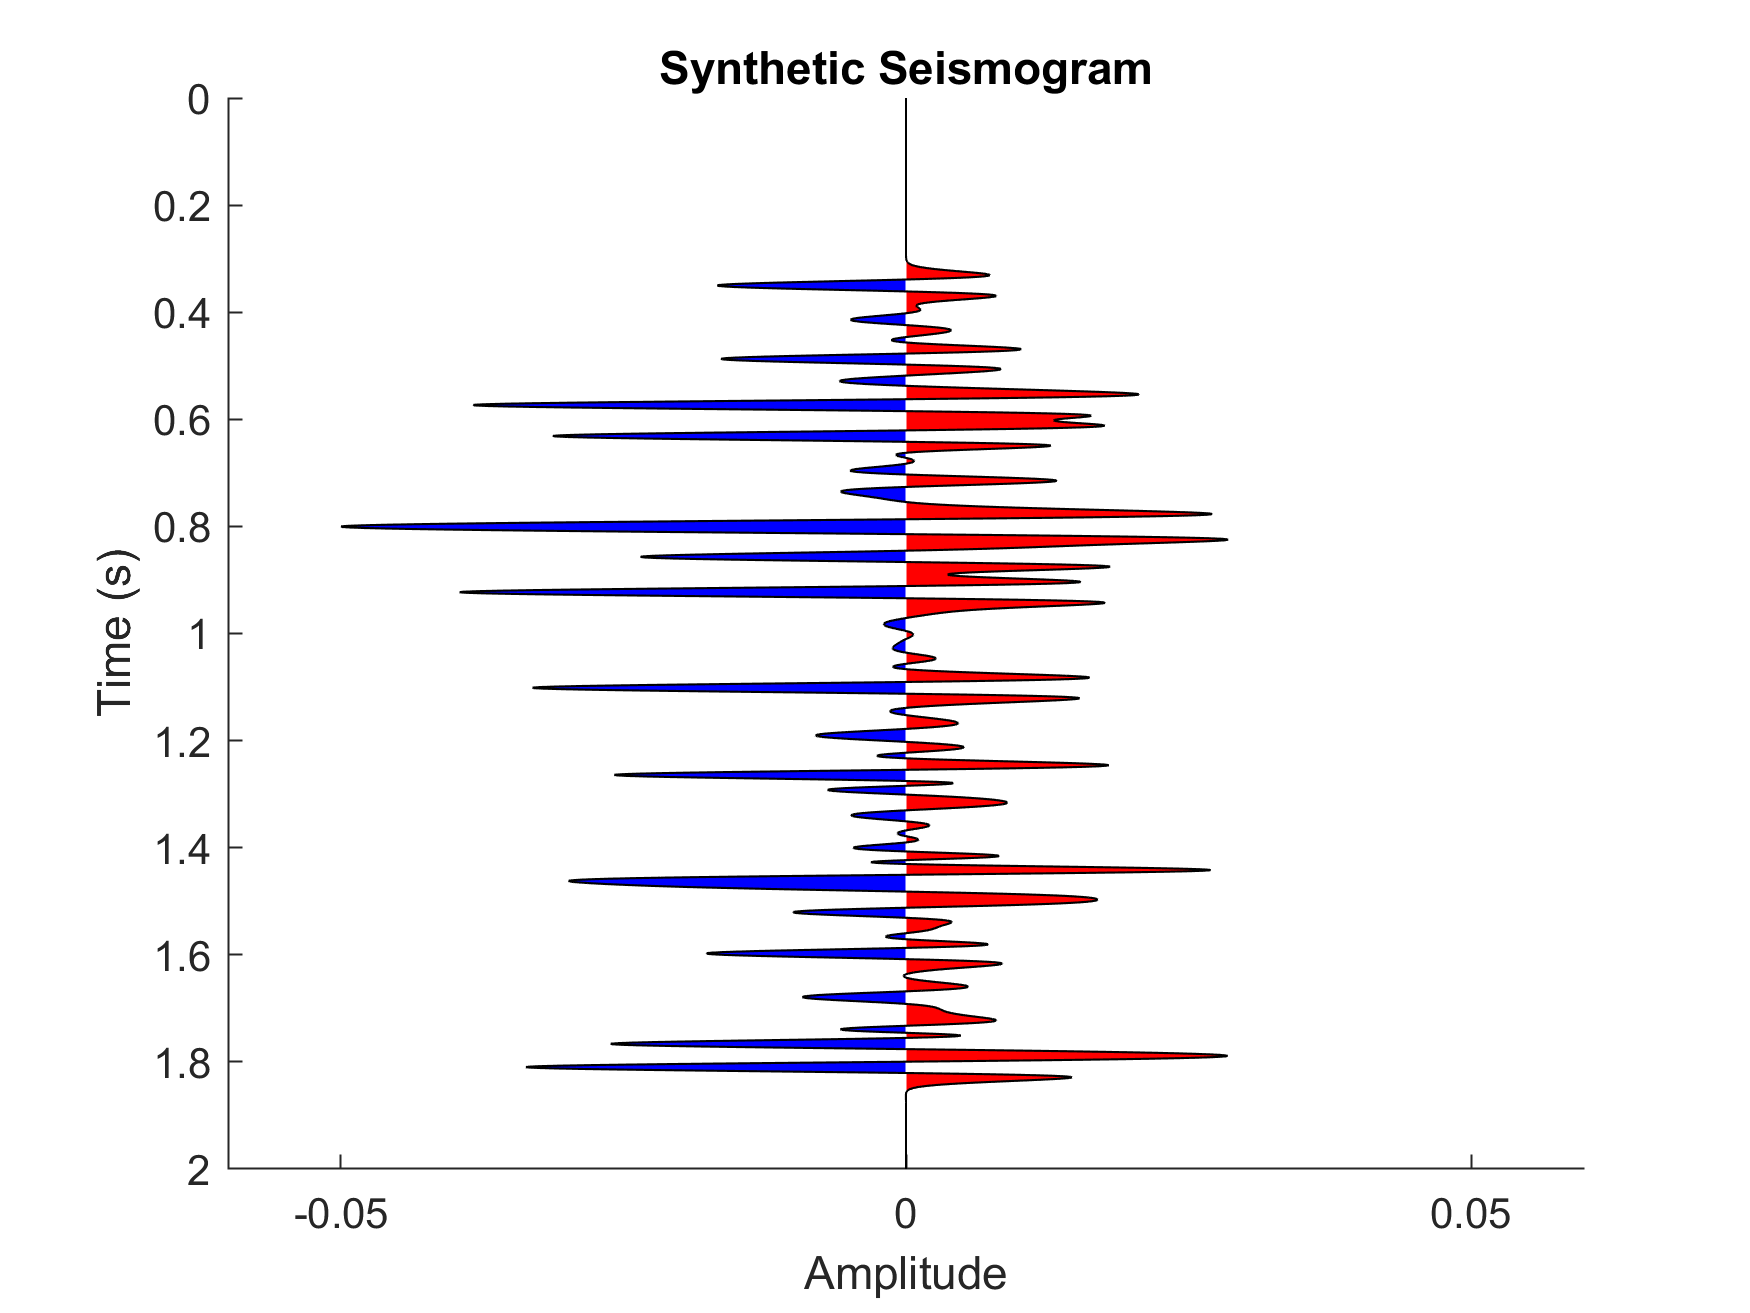
\includegraphics[width=0.7\textwidth]{Figures/RTCsyntheticPPr.png}
	\caption[Fox Creek ray-tracing P-P synthetic seismogram using a Ricker wavelet]{Synthetic seismogram for P-P reflections from ray-tracing using a $20 Hz$ zero-offset Ricker wavelet}
	\label{fig:RTCsyntheticPPr}
\end{figure}	

\begin{figure}[!htb]
	\centering
	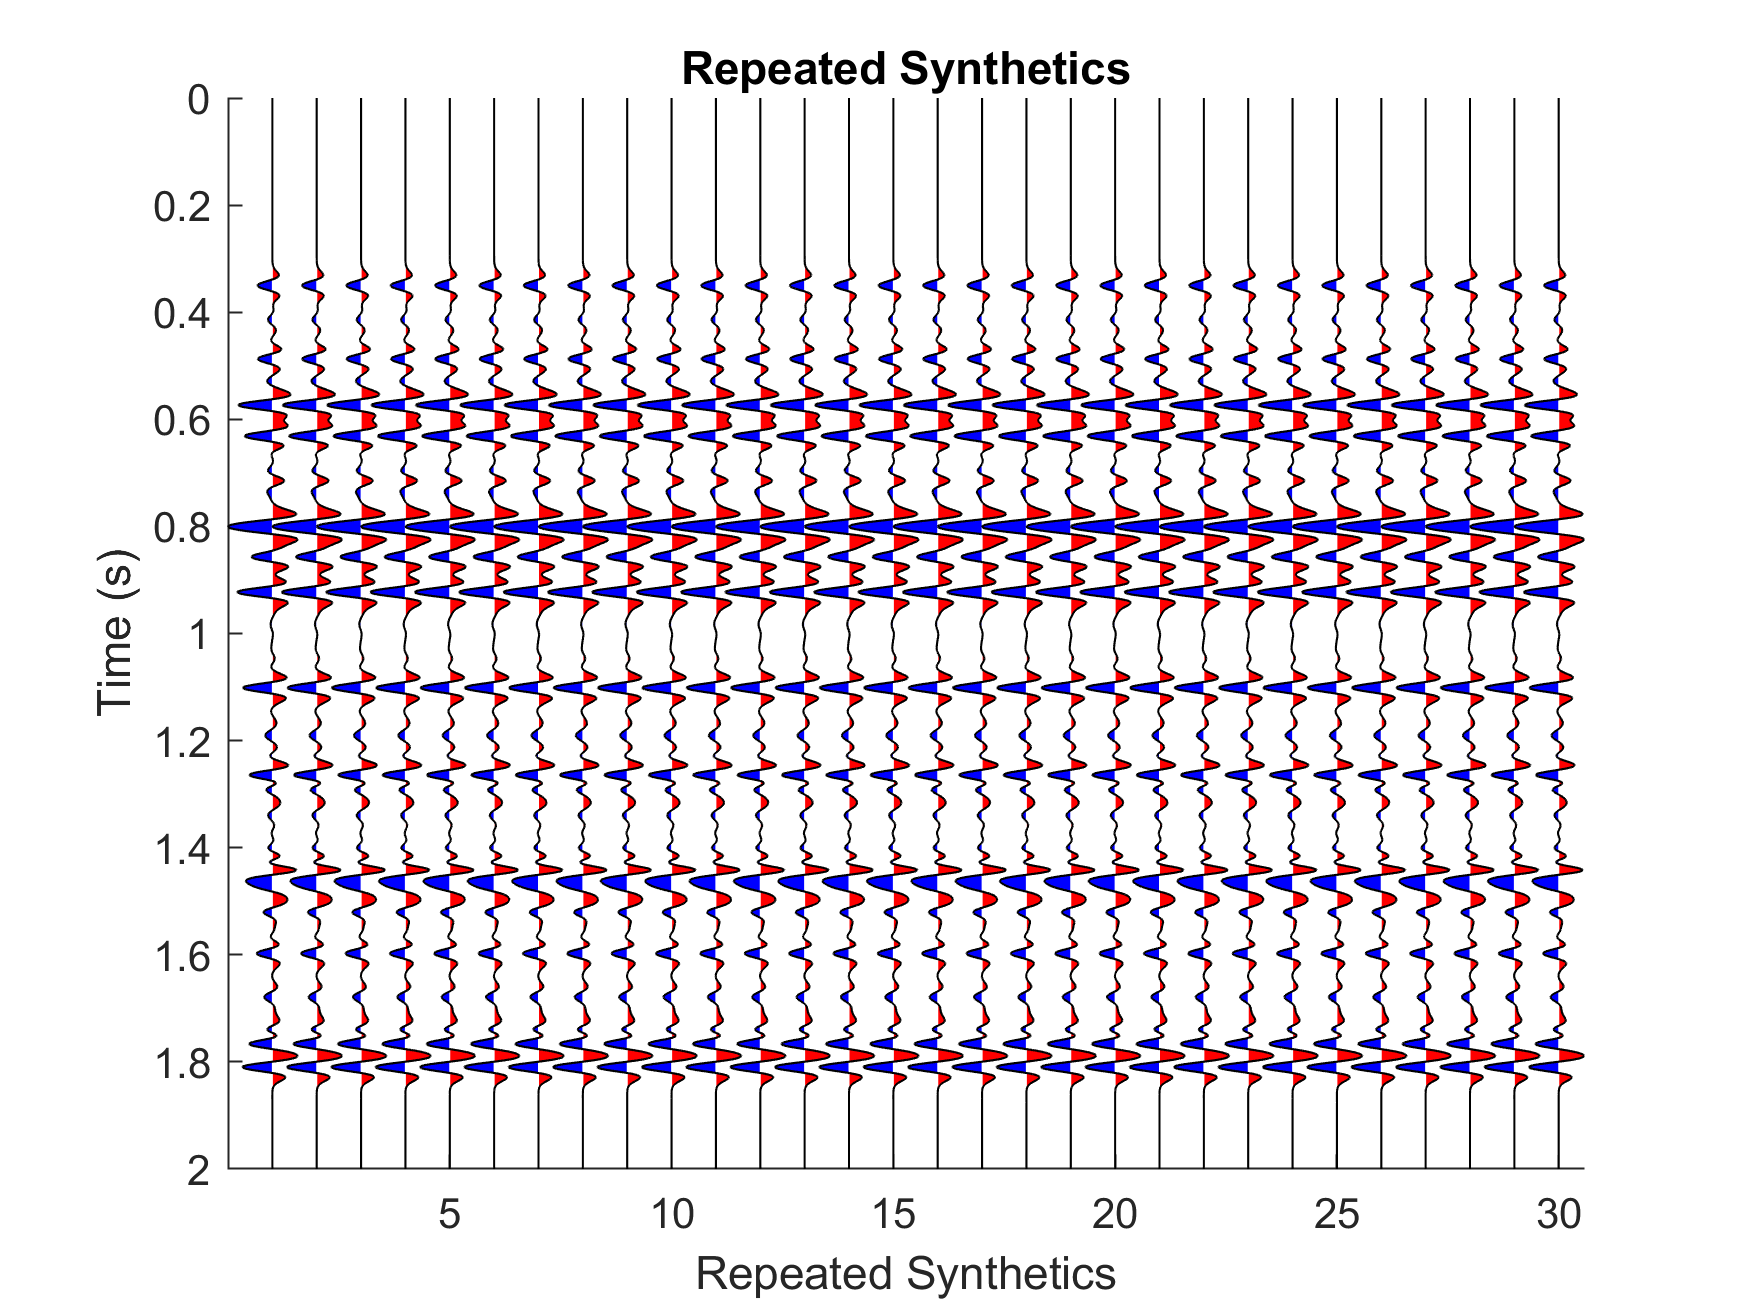
\includegraphics[width=0.7\textwidth]{Figures/RTCSeveralSyntheticsPPr.png}
	\caption[Fox Creek ray-tracing several P-P synthetic seismograms using a Ricker wavelet]{Several synthetic seismograms for P-P reflections from ray-tracing using a $20 Hz$ zero-offset Ricker wavelet}
	\label{fig:RTCSeveralSyntheticsPPr}
\end{figure}	

\FloatBarrier
\pagebreak









\end{document}
